\documentclass{article}
\usepackage[utf8]{inputenc}
\usepackage{capt-of} % Für captionof
\usepackage{hyperref} % Für Links

\title{Macherdaach-Badge \\ Lötanleitung \\ [1cm]
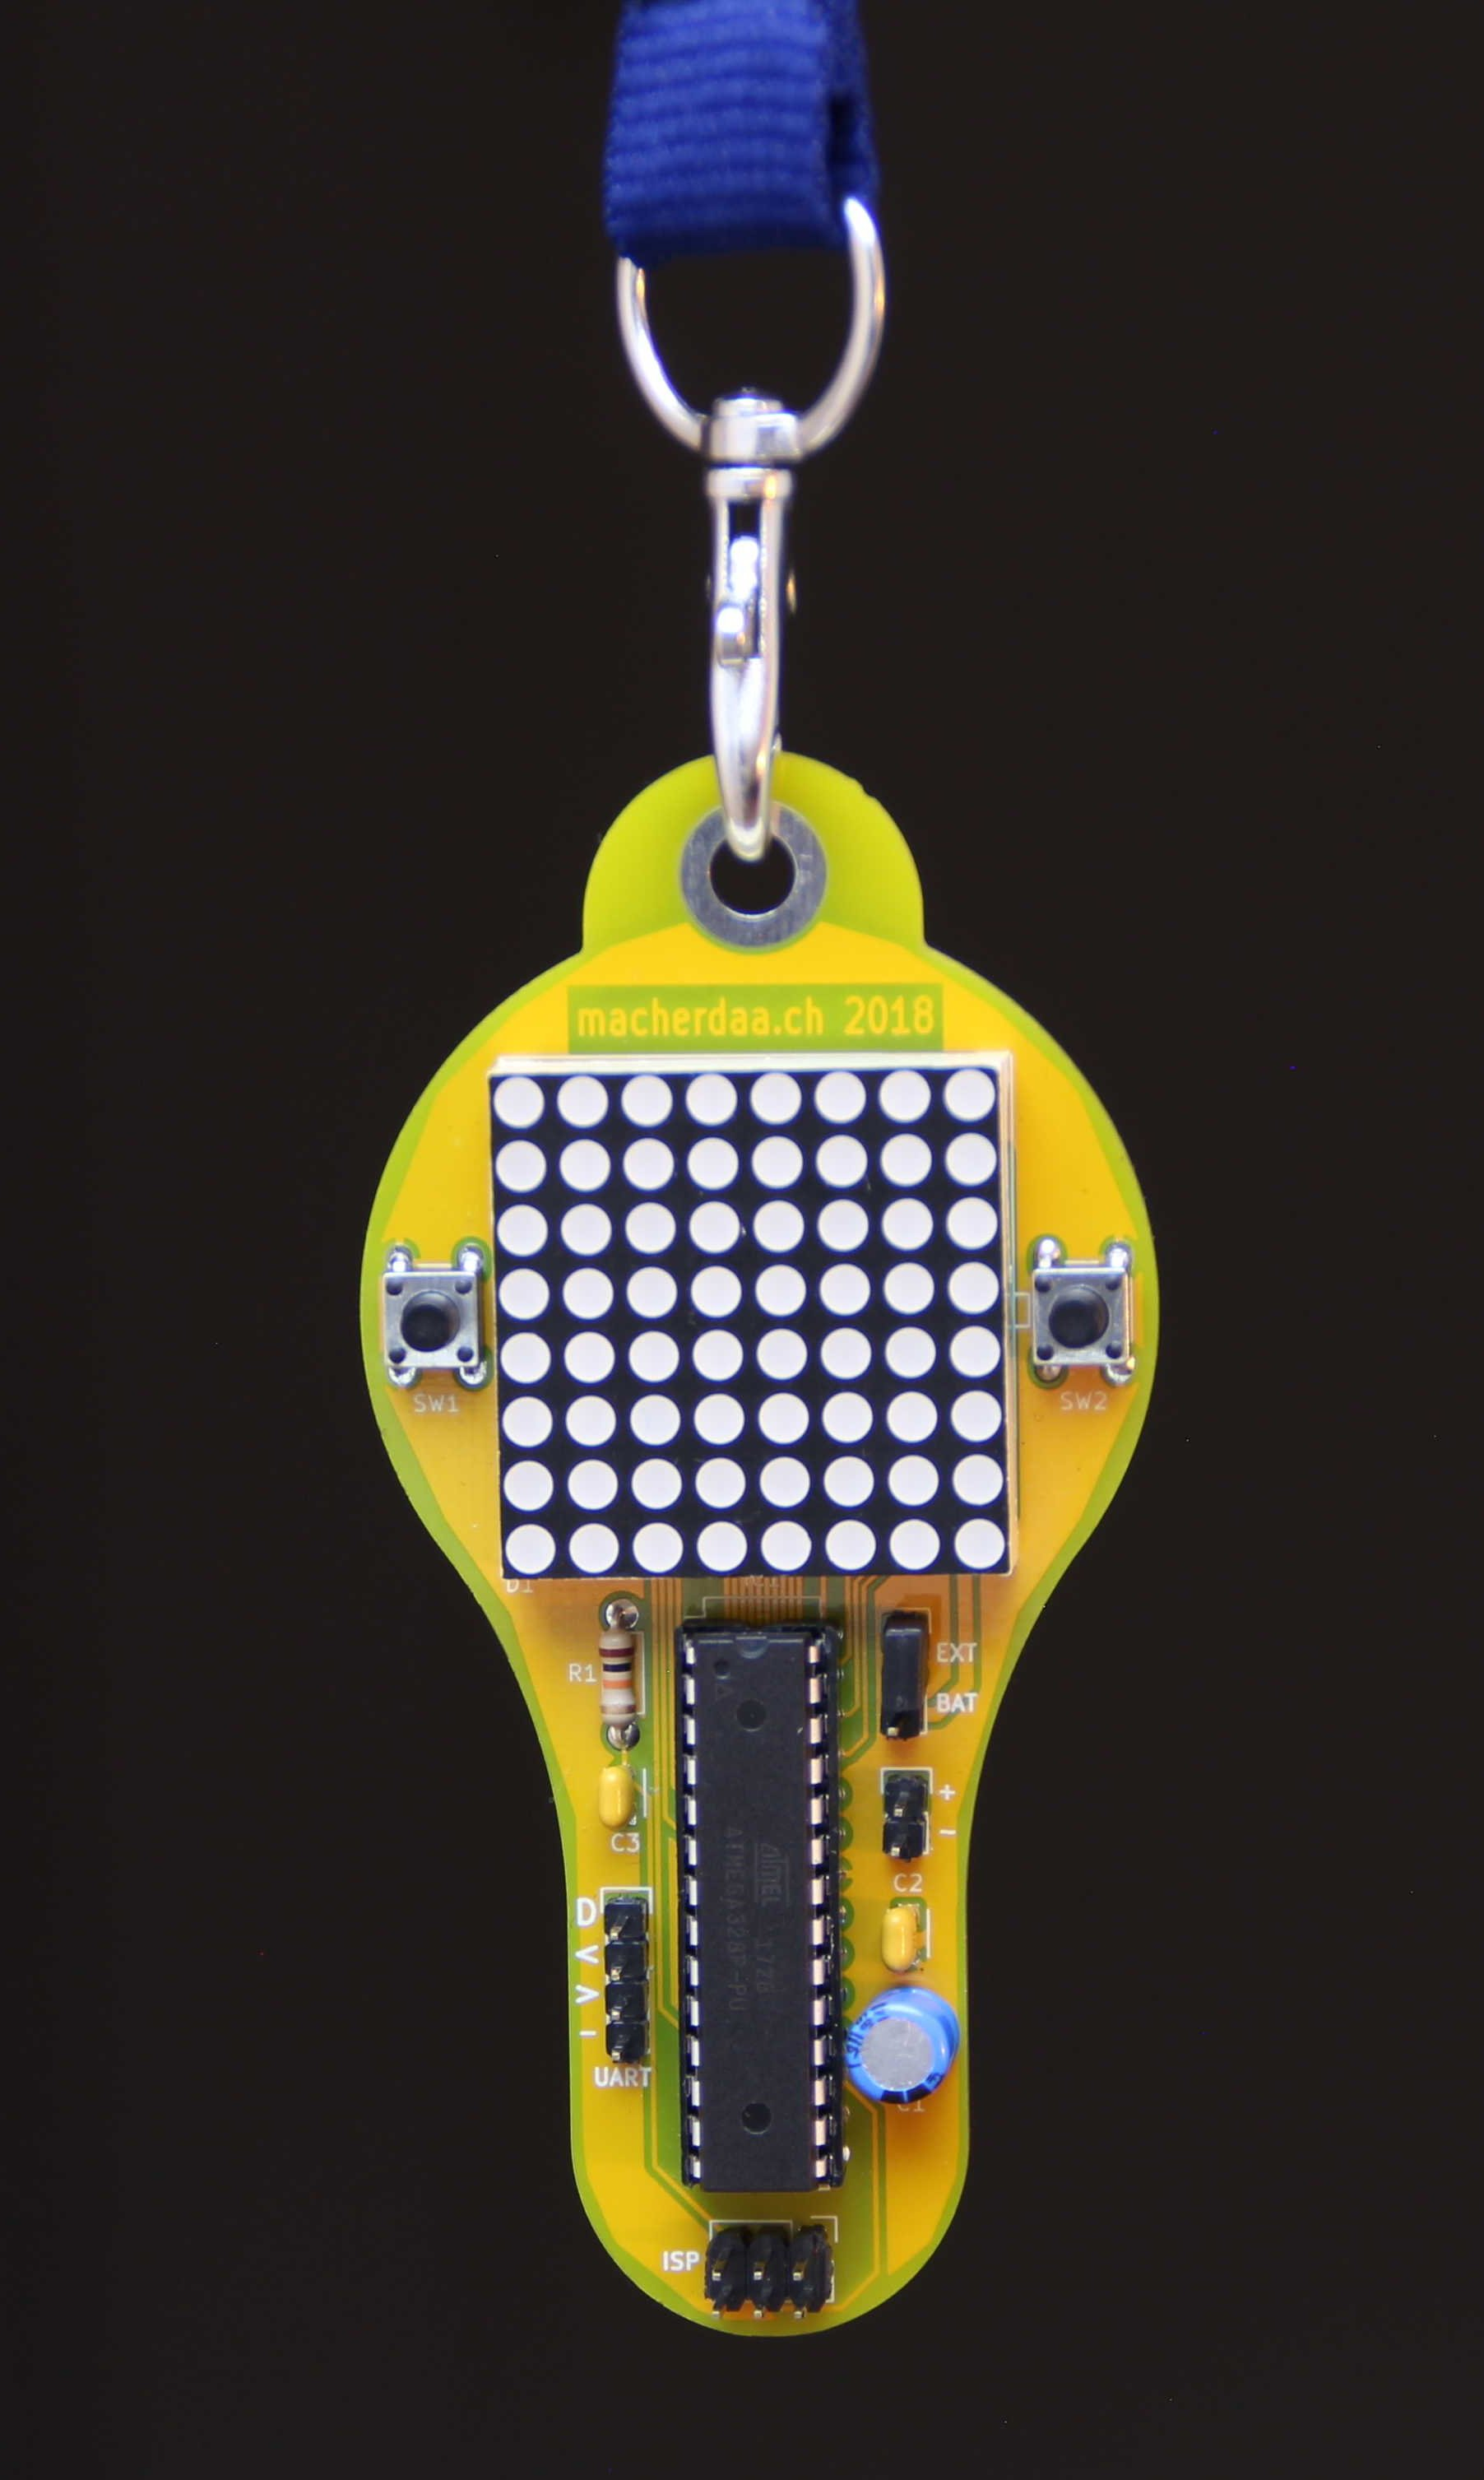
\includegraphics[width=0.5\textwidth]{Bilder/IMG_5645.JPG}
}
\date{Oktober 2018}
\author{casartar}

\usepackage{natbib}
\usepackage{graphicx}
\usepackage[ngerman]{babel} % Macht aus Figure -> Abbildung

\setlength{\parindent}{0pt} % Keine Einrückung nach Absatz

\usepackage{geometry} % Seitenränder ein bisschen schmaler
\geometry{
  left=2cm,
  right=2cm,
  top=2cm,
  bottom=2cm,
  bindingoffset=5mm
}

\begin{document}

\maketitle
\newpage
\section{Einleitung}

Das Macherdaach-Badge ist ein kleiner Bausatz zum selber zusammenlöten, der extra für den ersten Landauer Maker Day entwickelt wurde.
Du musst nur wenige Bauteile verlöten, bis du ein vollfunktionsfähes Badge dein Eigen nennen darfst. Neben coolen Mustern und ein paar Minispielen, wird in jedes Badge eine individuelle Laufschrift nur für dich einprogrammiert.\\

Wir wünschen viel Spaß und gutes Gelingen. 

\section{Die Bauteile stellen sich vor}
Alle Bauteile, die du für deinen Macherdaach-Badge brauchst, findest du in einer Tüte, die du von einem der freundlichen Helfer  am Tisch überreicht bekommst.

Folgende Bauteile sollten in der Tüte drin sein:

\begin{enumerate}
	\item Macherdaach Badge Platine
	\item LED-Matrix
	\item Mikrocontroller ATMEGA328P-PU
	\item Sockel für den Mikrocontroller
	\item Zwei Taster
	\item 10k$\Omega$ Widerstand
	\item Zwei 100nF Kondensatoren
	\item 100$\mu$F Elektrolytkondensator
	\item Einreihige Stiftleiste 2 Pins
	\item Einreihige Stiftleiste 3 Pins
	\item Einreihige Stiftleiste 4 Pins
	\item Zweireihige Stiftleiste 3 Pins
	\item Jumper
	\item Knopfzellenhalter
	\item Knopfzelle CR2032
\end{enumerate}



\begin{center}
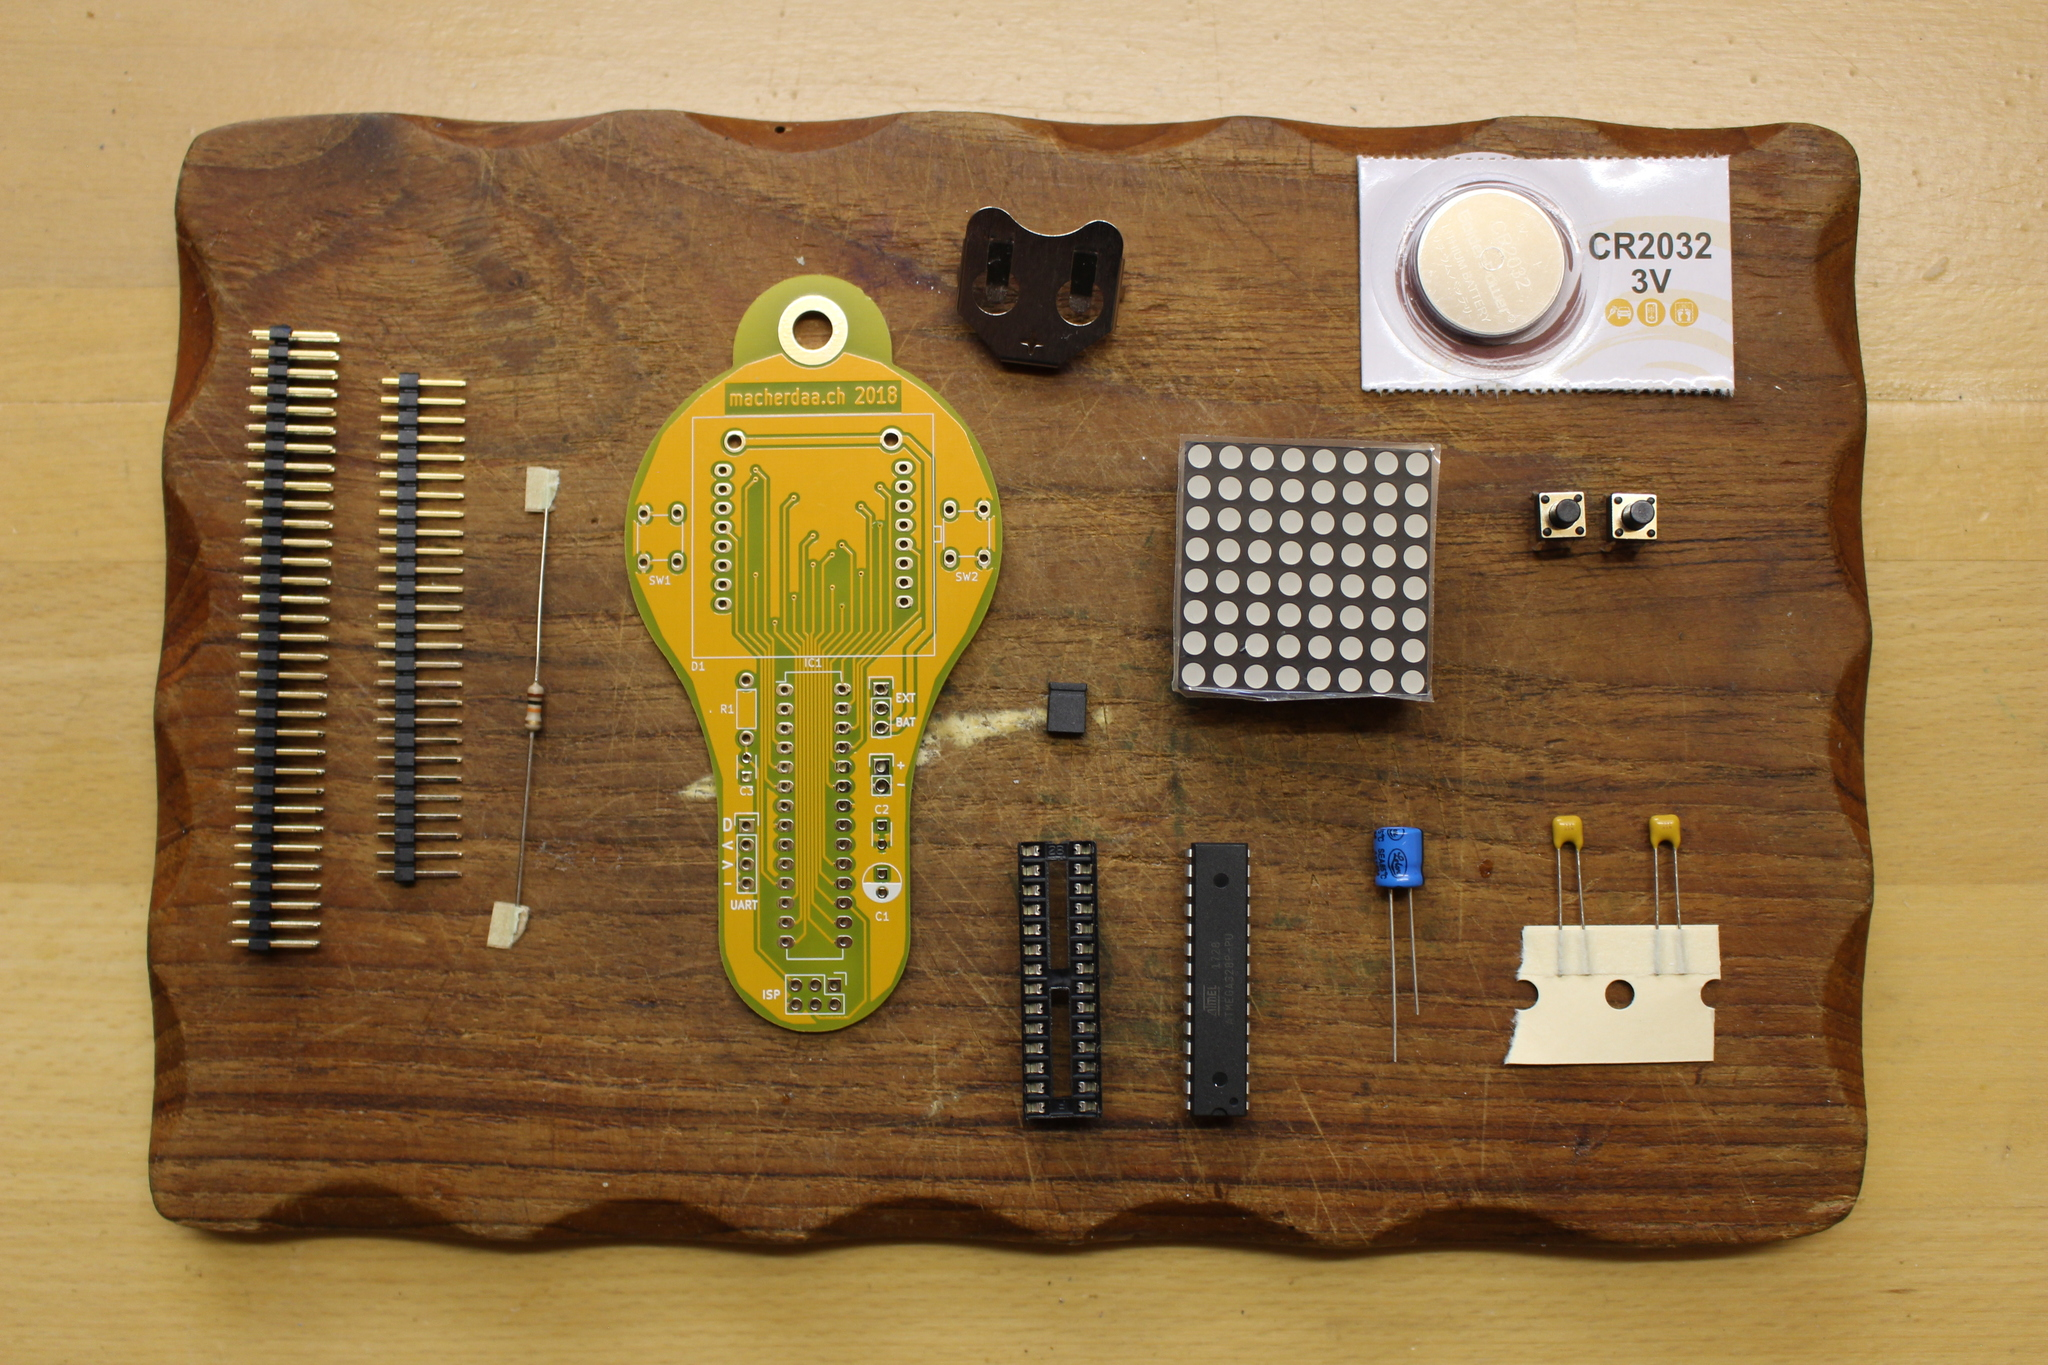
\includegraphics[width=\textwidth]{Bilder/IMG_5537.JPG}
\captionof{figure}{Alle Bauteile auf einen Blick}
\label{fig:all_components}
\end{center}

\section{Die Option für weniger Arbeit}

Wenn du dir sicher bist, dass du den Macherdaach-Badge zu Hause nicht neu programmieren möchtest, dann kannst du den Widerstand R1, den Kondensator C3 und alle Stiftleisten, außer der einreihigen mit drei Pins, beim Zusammenlöten auch weglassen.

Diese Bauteile sind nur zum Programmieren des Mikrocontrollers, nicht aber für die normale Funktion notwendig.

\section{Dokumentation ist alles}

Die Hardware, Software und selbstverständlich diese Anleitung sind Open Source. Wenn du sie dir ansehen, sie herunterladen oder daran mitarbeiten möchtest, musst du nur folgenden Links folgen:

\begin{itemize}
	\item \url{https://github.com/casartar/MacherDaachBadgeFirmware}
	\item \url{https://github.com/casartar/MacherDaachBadgeHardware}
	\item \url{https://github.com/casartar/MacherDaachBadgeDoku}
\end{itemize}

Oder suche auf github.com nach Macherdaach.

\section{Jetzt geht es richtig los}
Wir löten die Bauteile nach der Regel: Das niedrigste Bauteil zu erst.

\subsection{Widerstand - R1 (100k$\Omega$)}
Zuerst nimmst du den 10k$\Omega$ Widerstand und biegst die Anschlussdrähte nach unten. Dabei musst du darauf achten, die Drähte direkt am Gehäuse zu biegen sonst passen sie später nicht richtig in die Bohrlöcher. Anschließend steckst du den Widerstand an die mit R1 markierte Stelle auf der Platine.

Dann legst du die Platine so hin, dass der Widerstand gegen das Brett gedrückt wird und verlötest die beiden Beinchen.

Zum Schluss müssen die überstehenden Beinchen noch mit der Zange abgezwickt werden.

\vspace{1cm}

\begin{minipage}[b]{0.5\textwidth}
	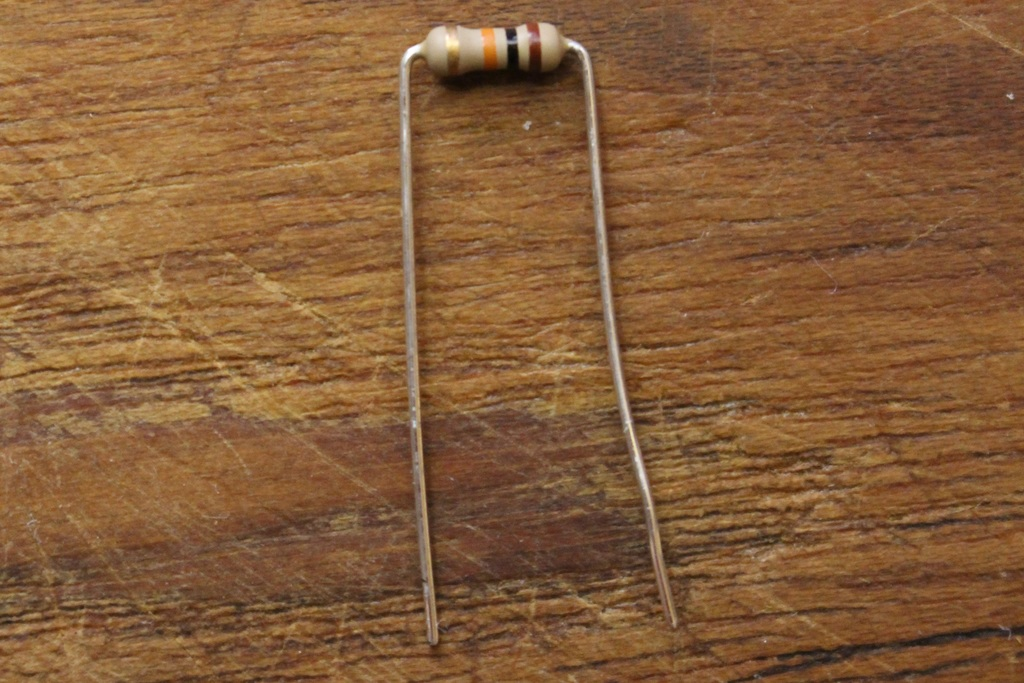
\includegraphics[width=\textwidth]{Bilder/IMG_5538.JPG}
	%\captionof{figure}{}
	%\label{fig:}
\end{minipage}
\begin{minipage}[b]{0.5\textwidth}
	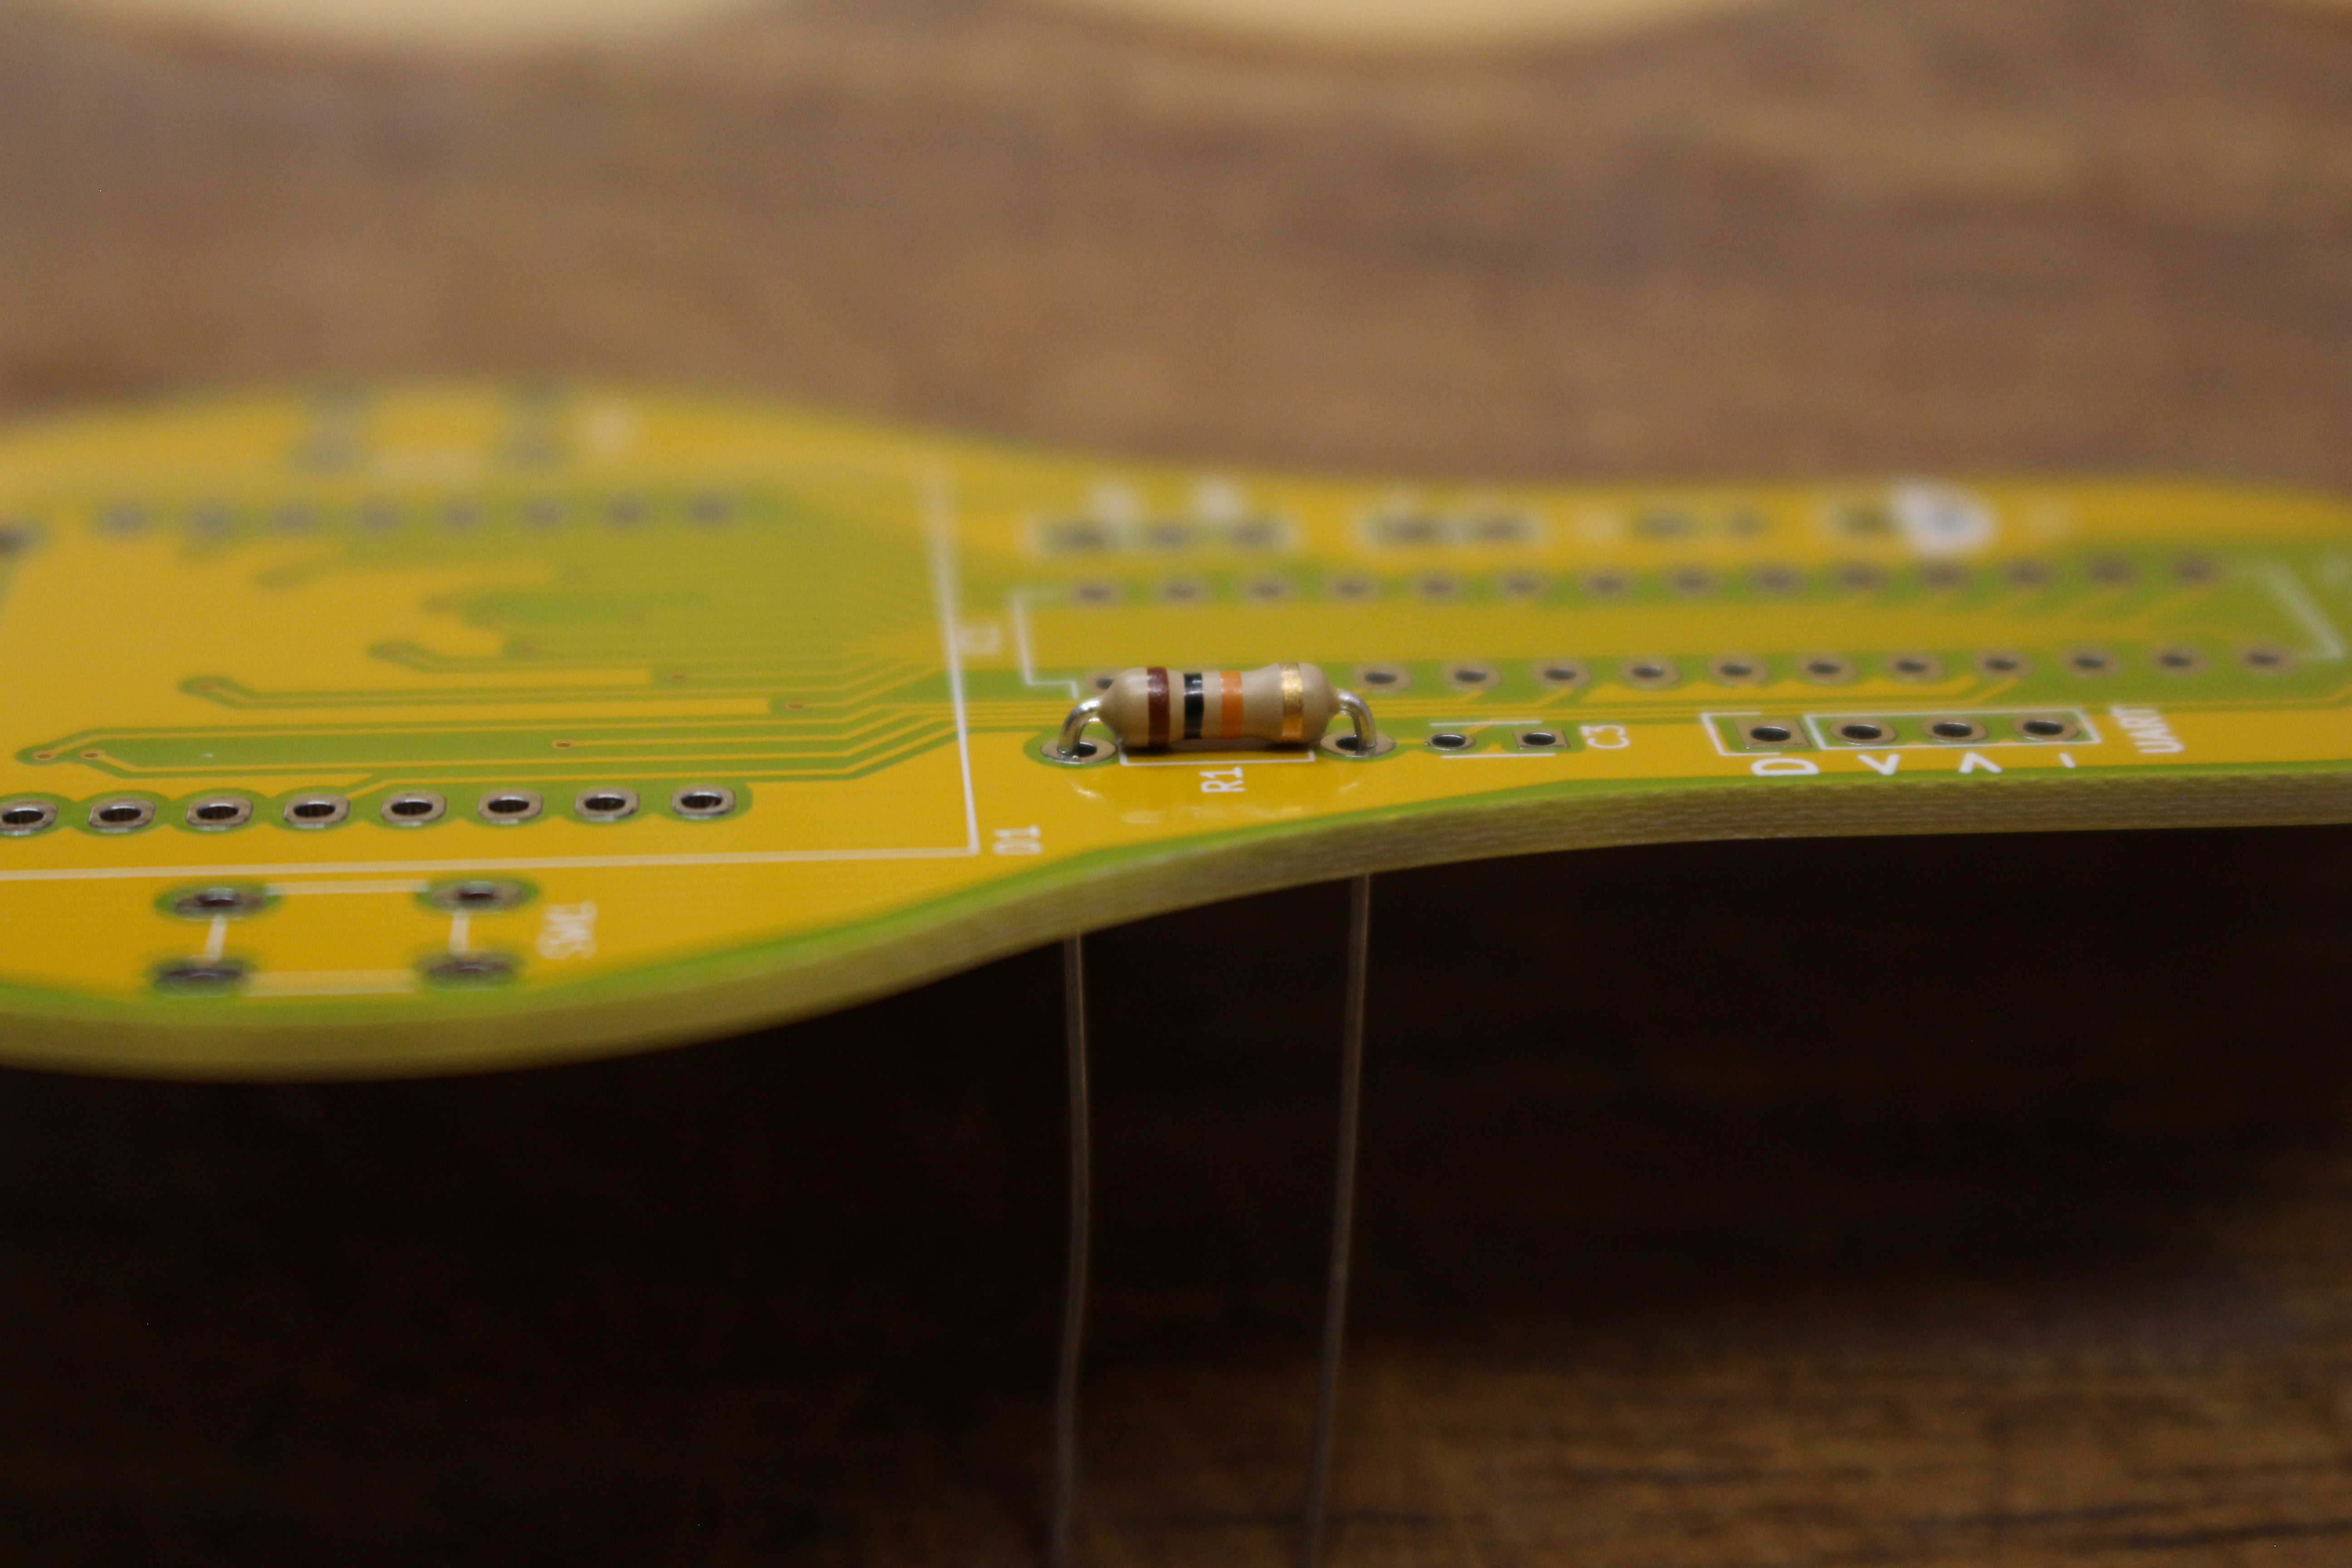
\includegraphics[width=\textwidth]{Bilder/IMG_5539.JPG}
	%\captionof{figure}{}
	%\label{fig:}
\end{minipage}

\vspace{0.5cm}

\begin{minipage}[b]{0.5\textwidth}
	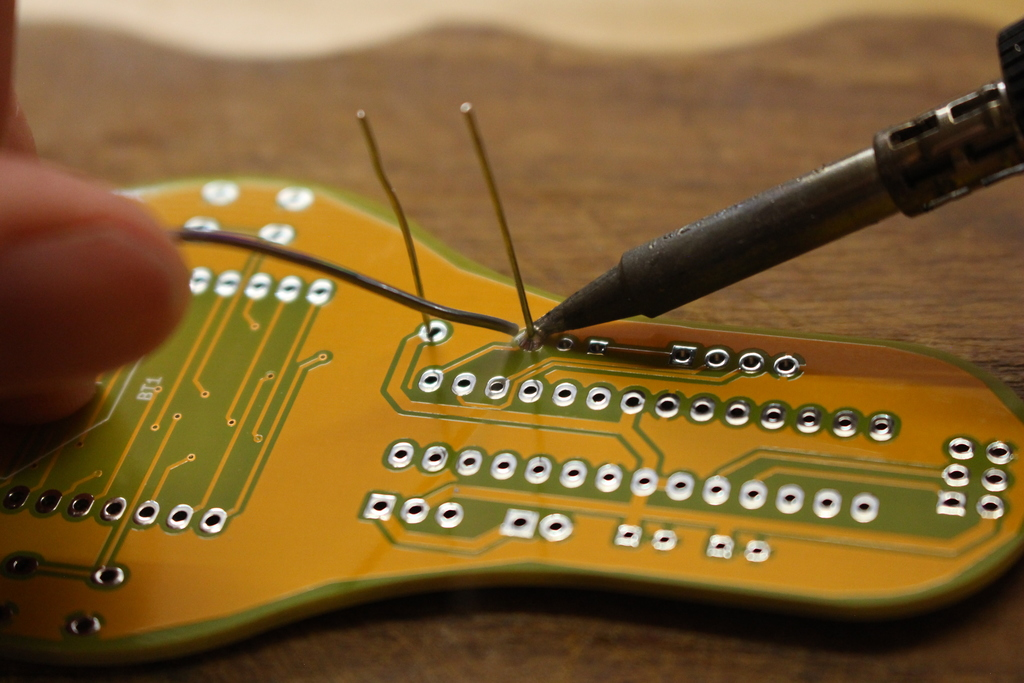
\includegraphics[width=\textwidth]{Bilder/IMG_5542.JPG}
	%\captionof{figure}{}
	%\label{fig:}
\end{minipage}
\begin{minipage}[b]{0.5\textwidth}
	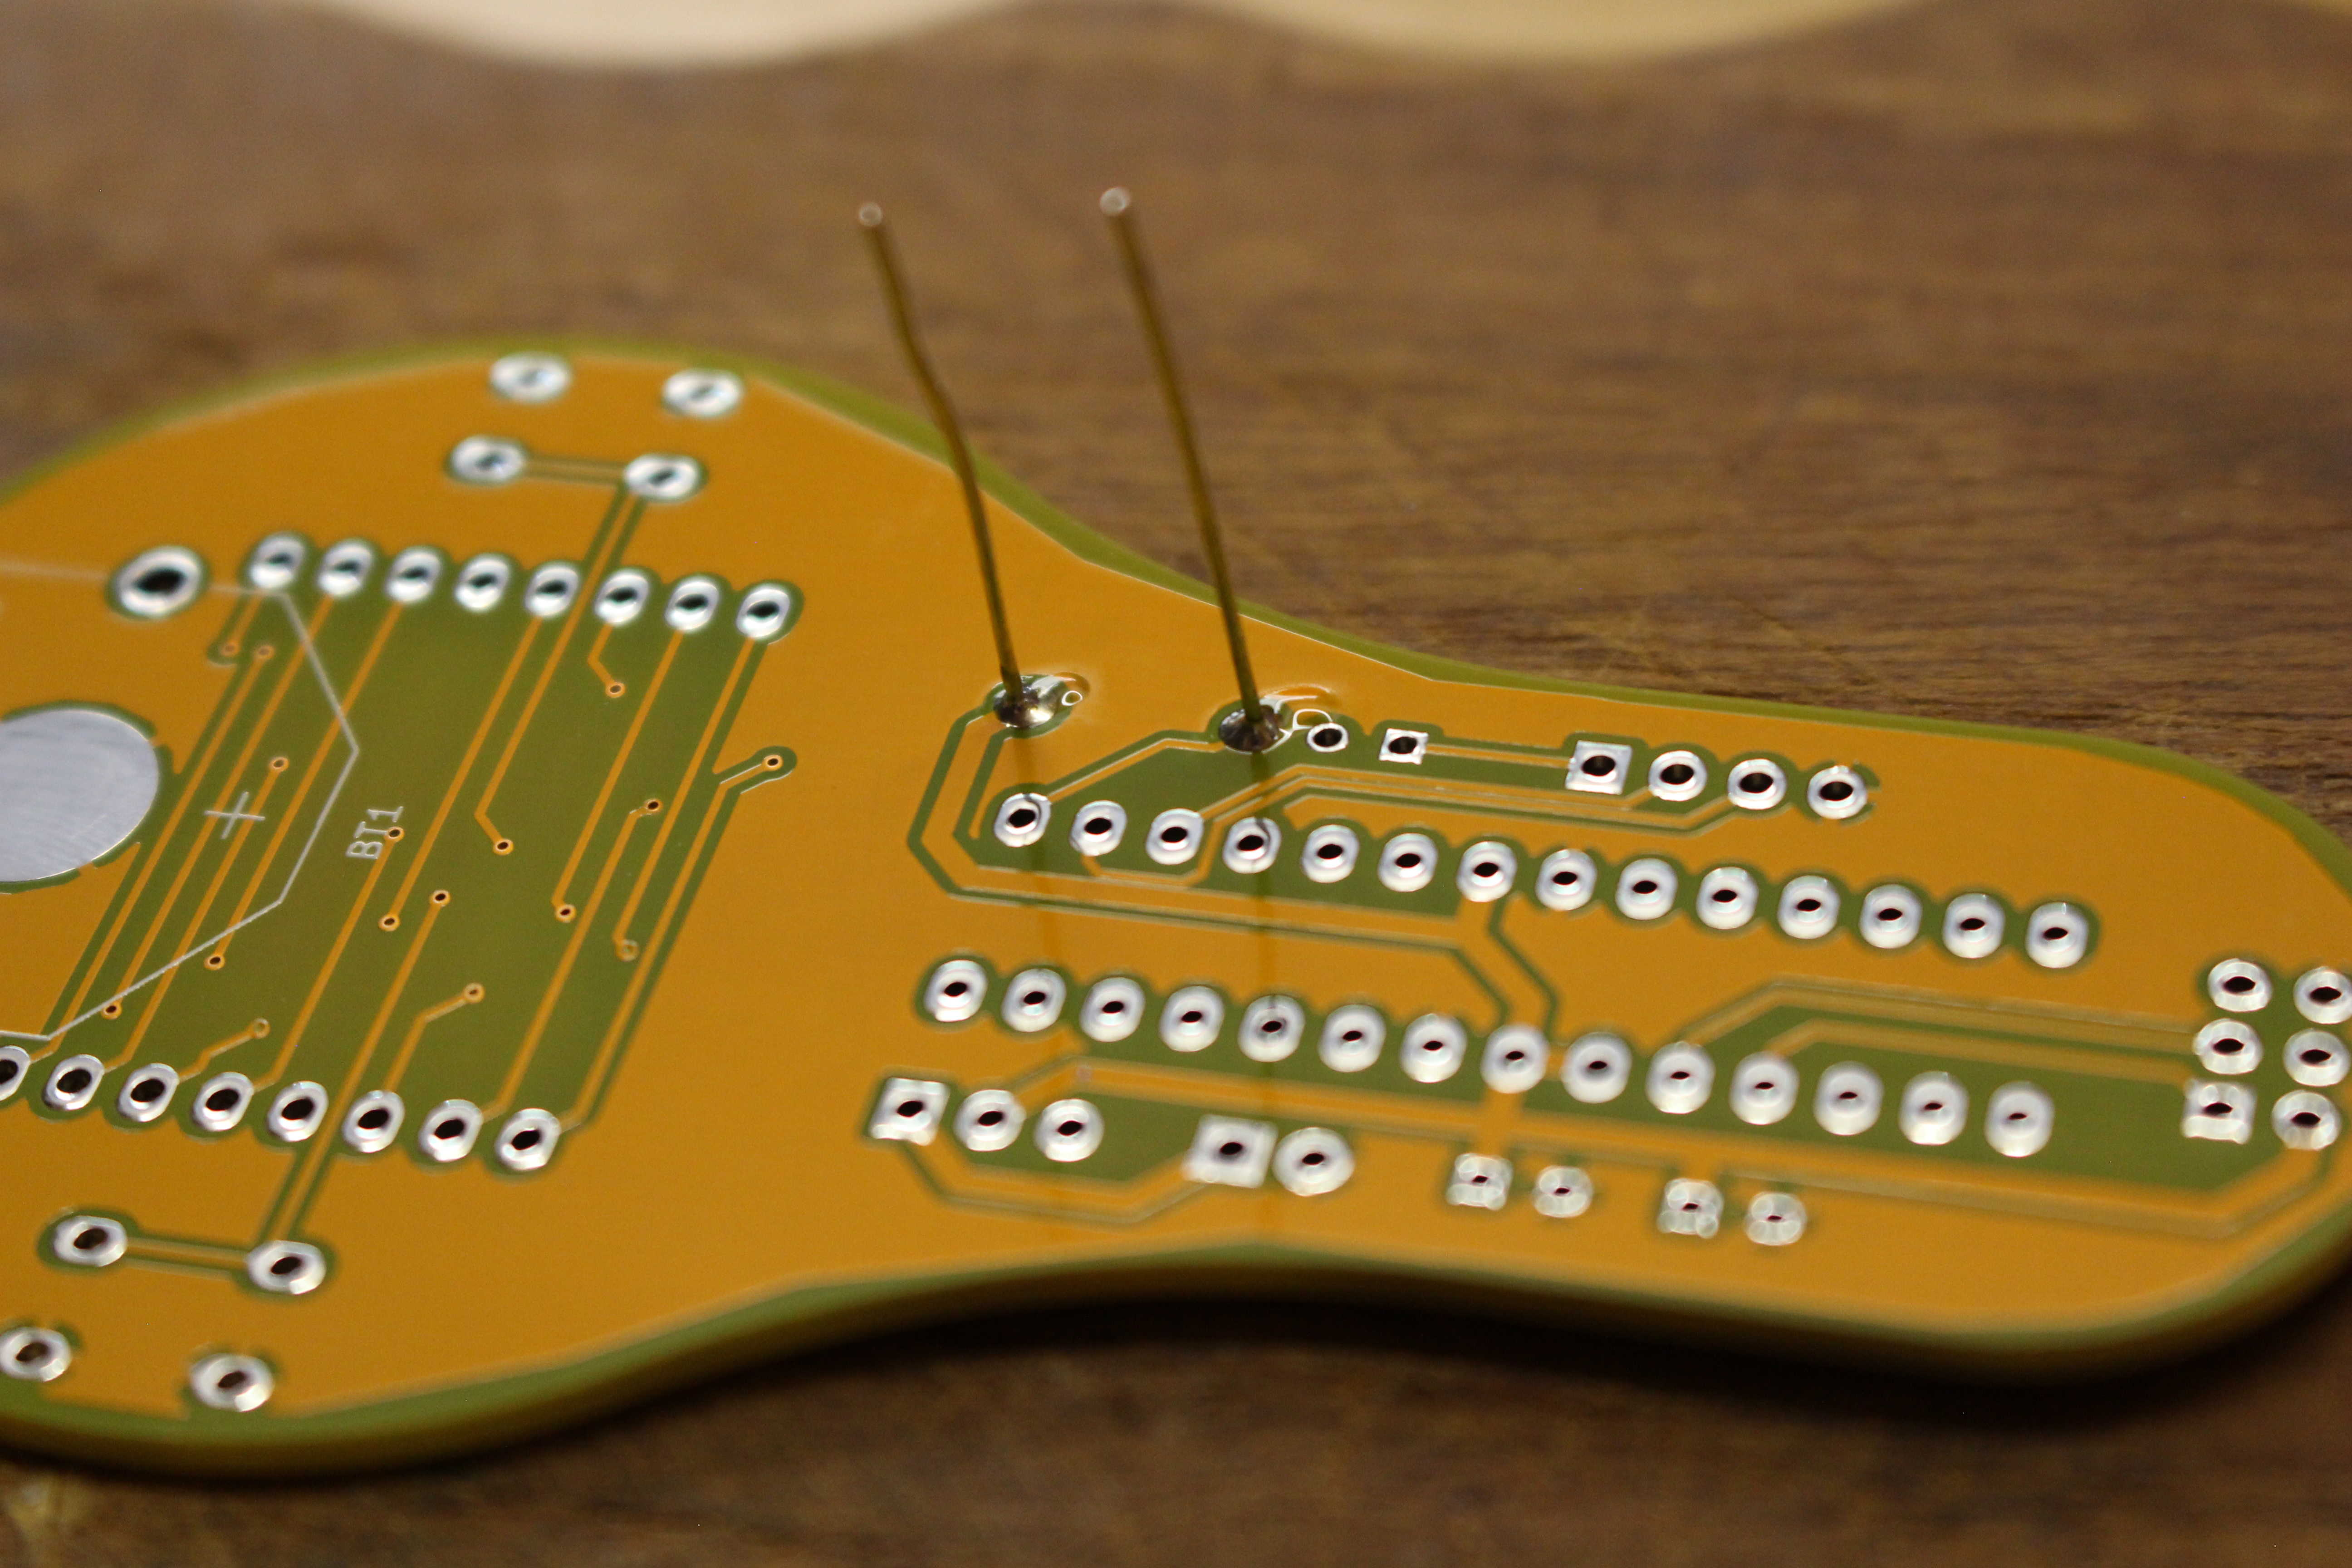
\includegraphics[width=\textwidth]{Bilder/IMG_5543.JPG}
	%\captionof{figure}{}
	%\label{fig:}
\end{minipage}

\vspace{0.5cm}

\begin{minipage}[b]{0.5\textwidth}
	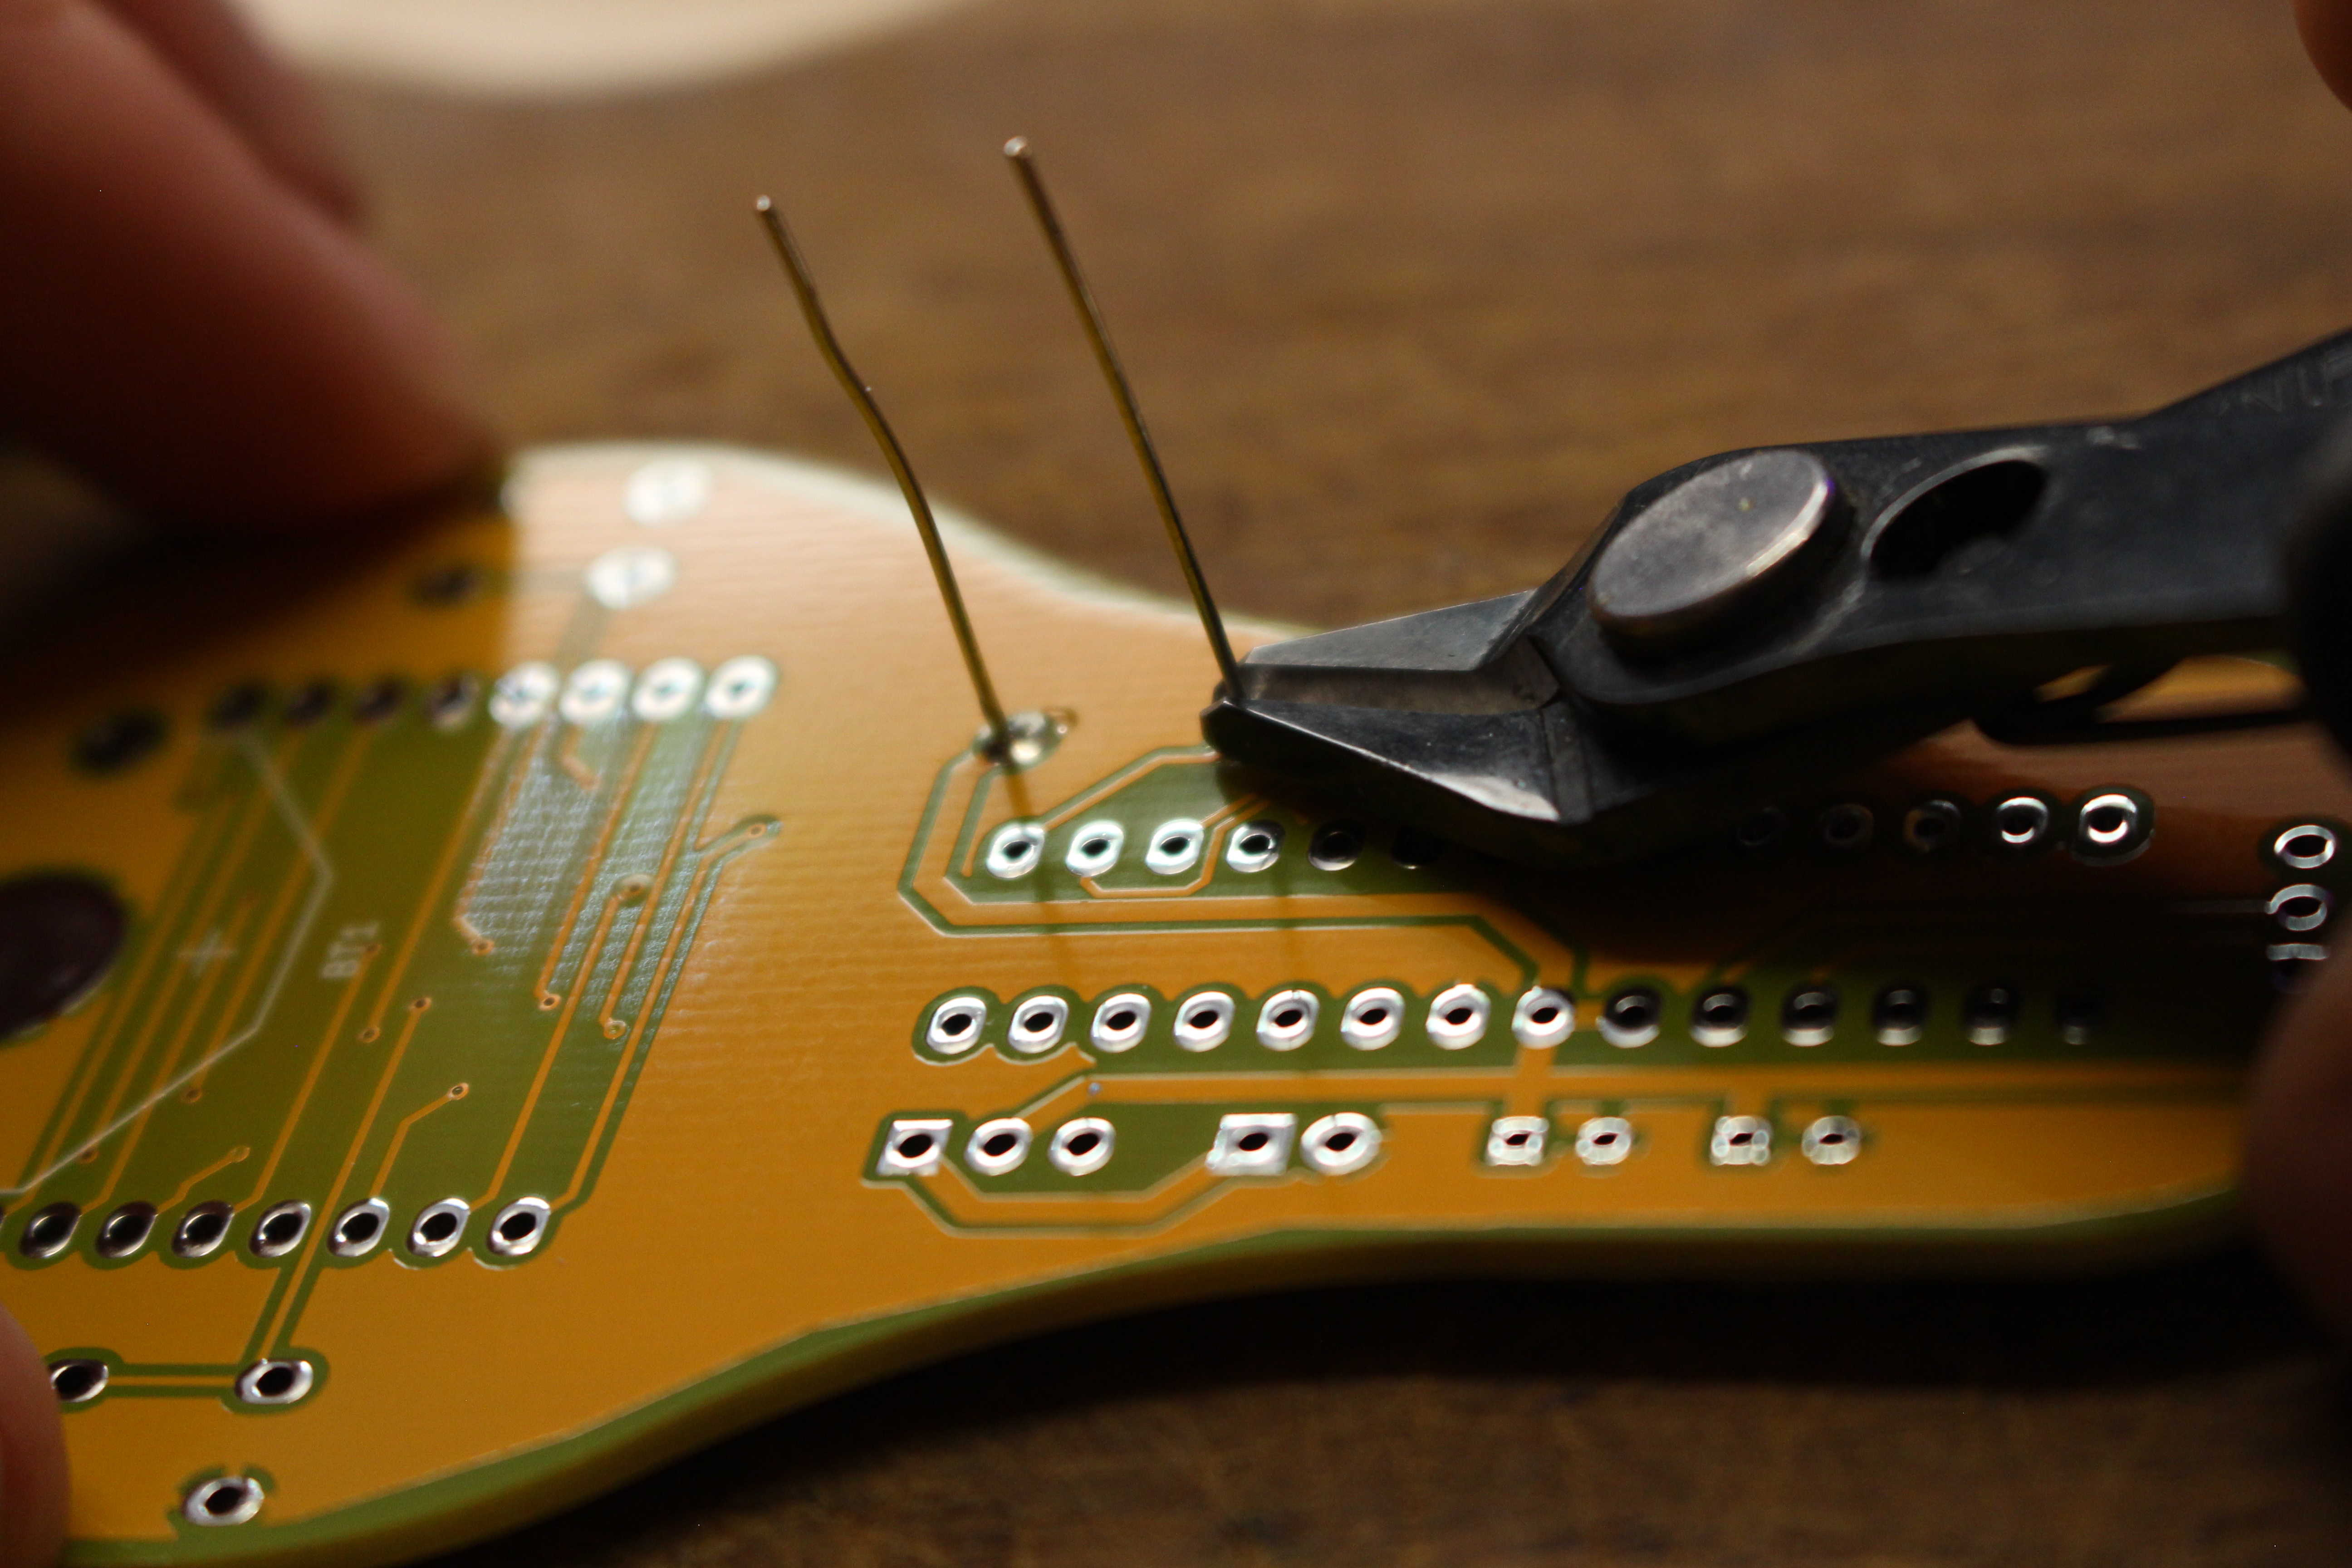
\includegraphics[width=\textwidth]{Bilder/IMG_5544.JPG}
	%\captionof{figure}{}
	%\label{fig:}
\end{minipage}
\begin{minipage}[b]{0.5\textwidth}
	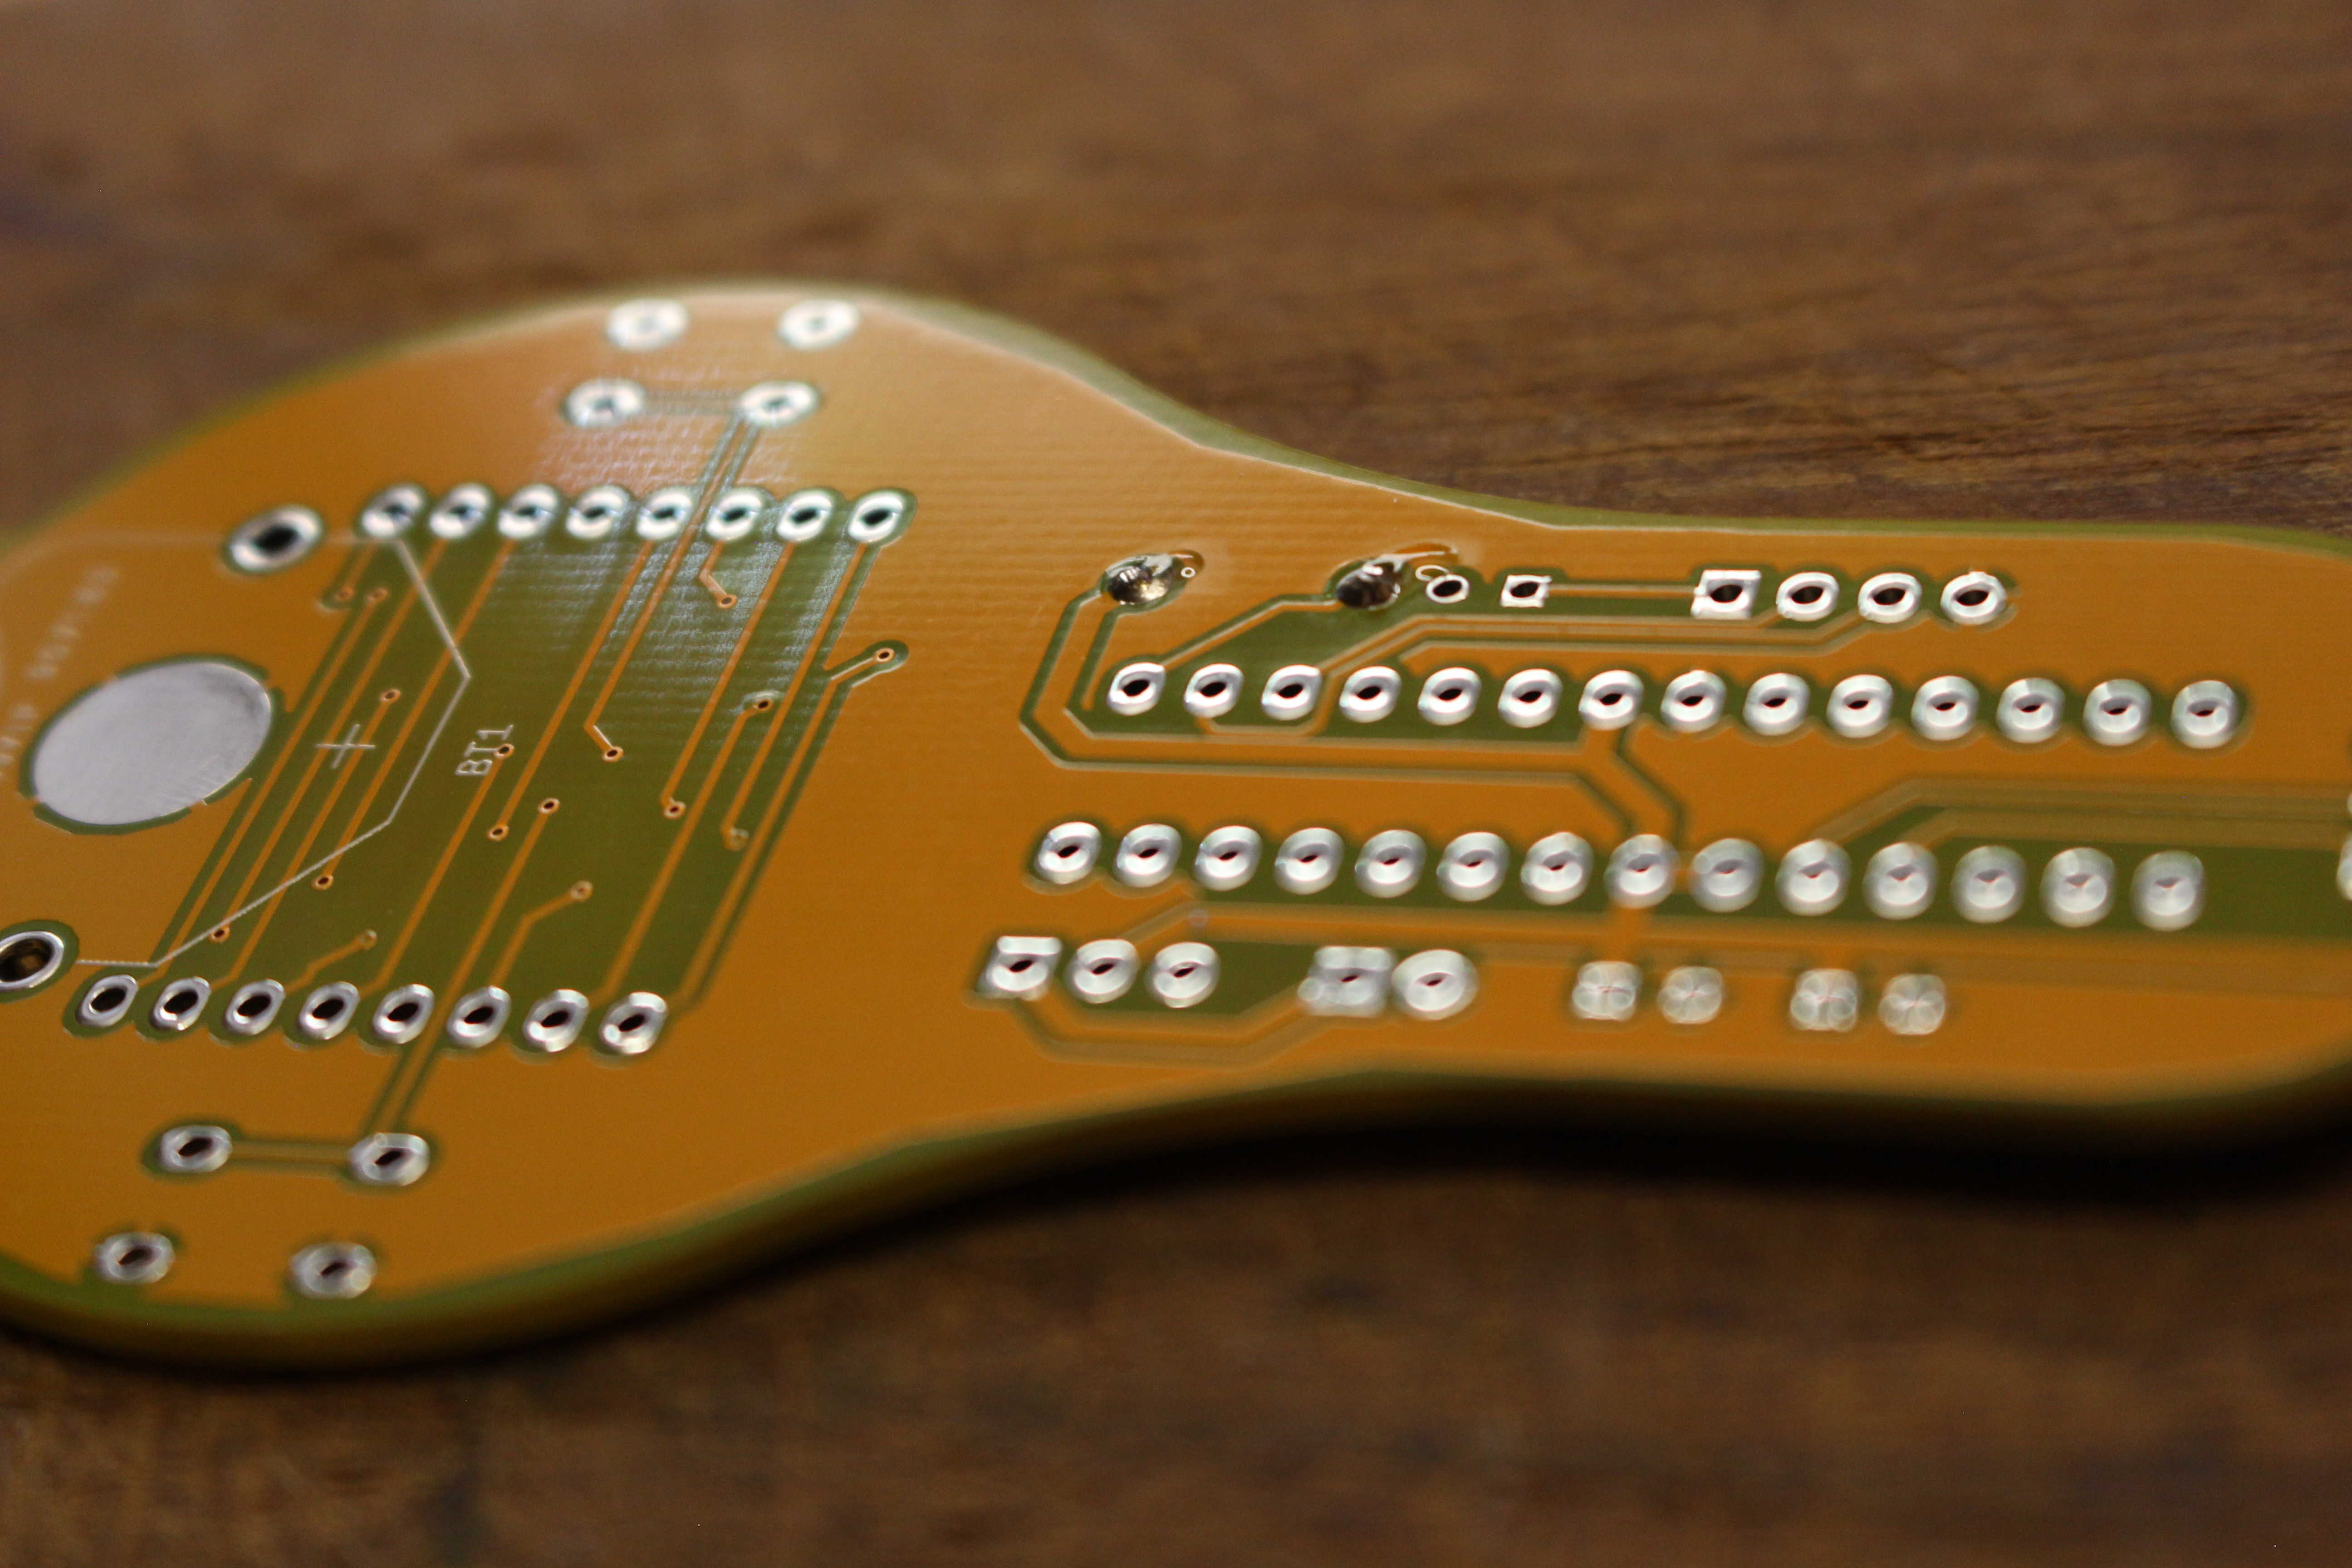
\includegraphics[width=\textwidth]{Bilder/IMG_5545.JPG}
	%\captionof{figure}{}
	%\label{fig:}
\end{minipage}

\subsection{Kondensatoren - C2 und C3 (100nF)}

Als nächstes kommen nacheinander die beiden 100nF Kondensatoren dran.
Das funktioniert genau wie beim Widerstand, nur das die Anschlussdrähte schon in die richtige Richtung zeigen.

\vspace{1cm}

\begin{minipage}[b]{0.5\textwidth}
	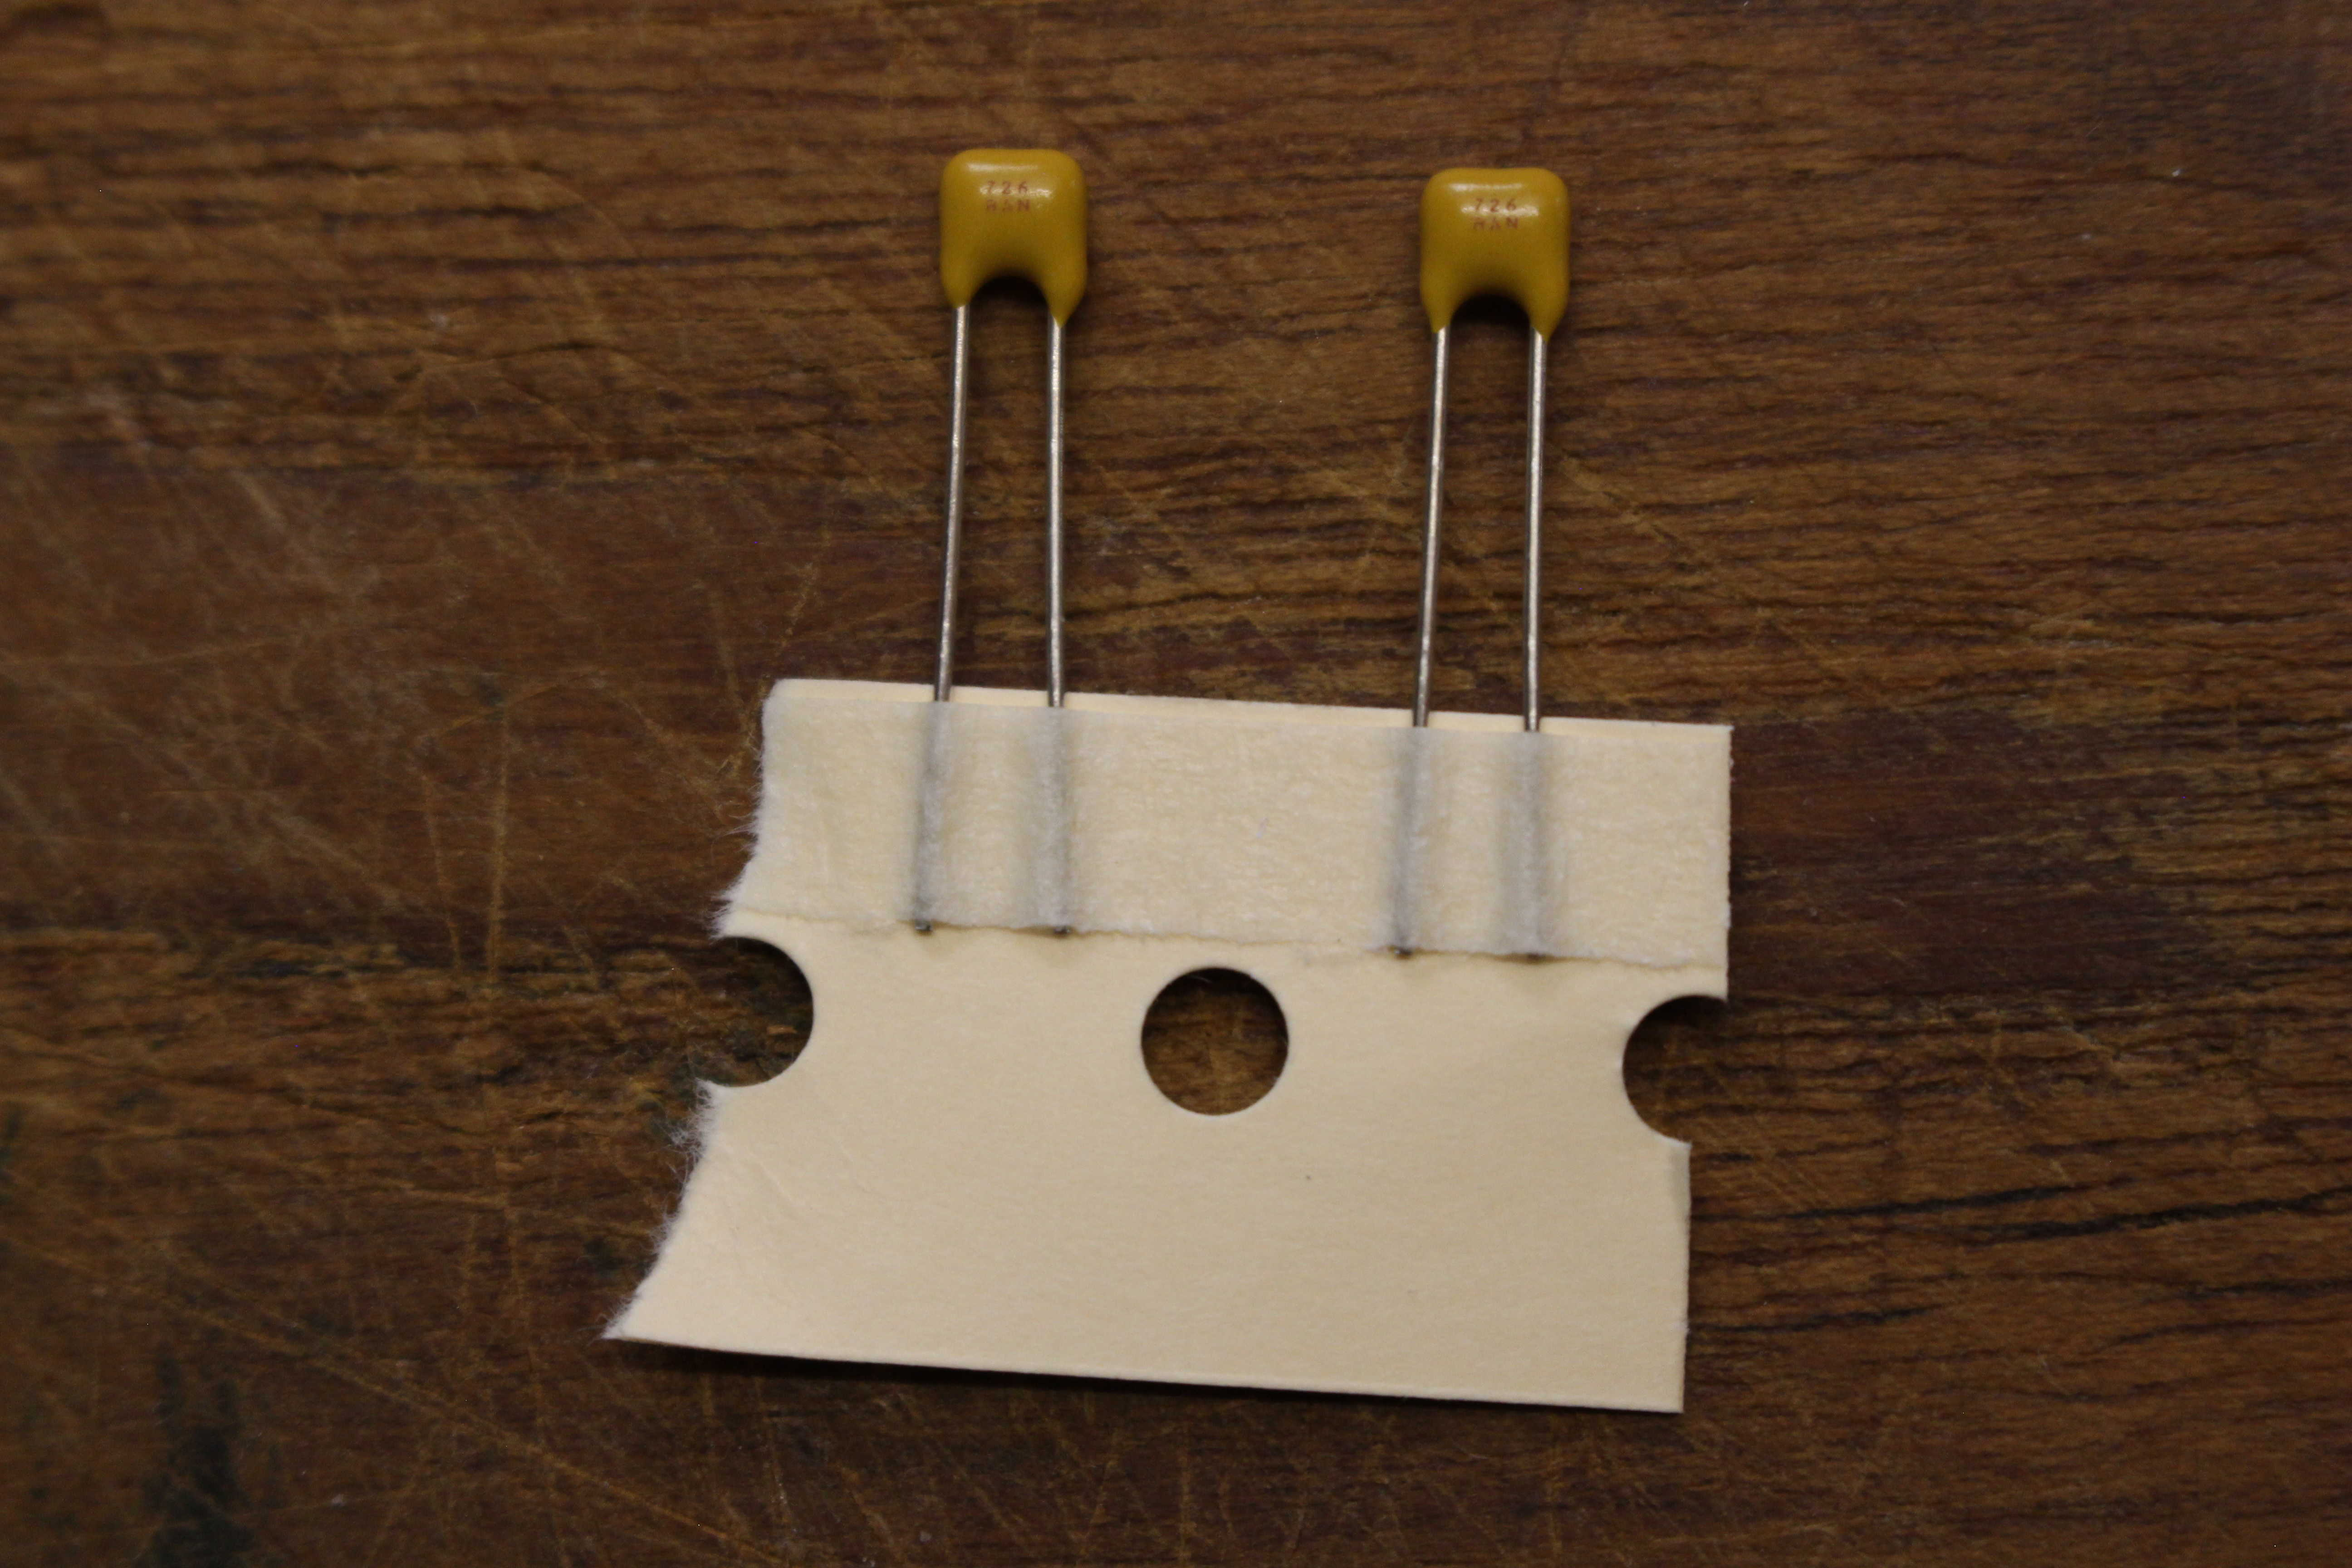
\includegraphics[width=\textwidth]{Bilder/IMG_5546.JPG}
	%\captionof{figure}{}
	%\label{fig:}
\end{minipage}
\begin{minipage}[b]{0.5\textwidth}
	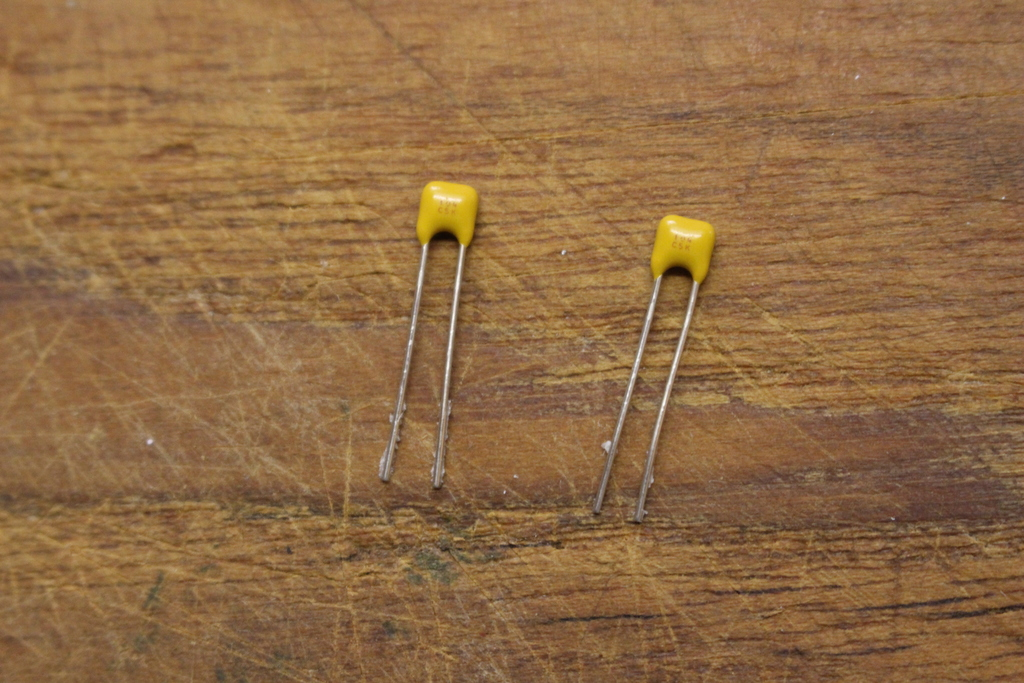
\includegraphics[width=\textwidth]{Bilder/IMG_5547.JPG}
	%\captionof{figure}{}
	%\label{fig:}
\end{minipage}

\vspace{0.5cm}

\begin{minipage}[b]{0.5\textwidth}
	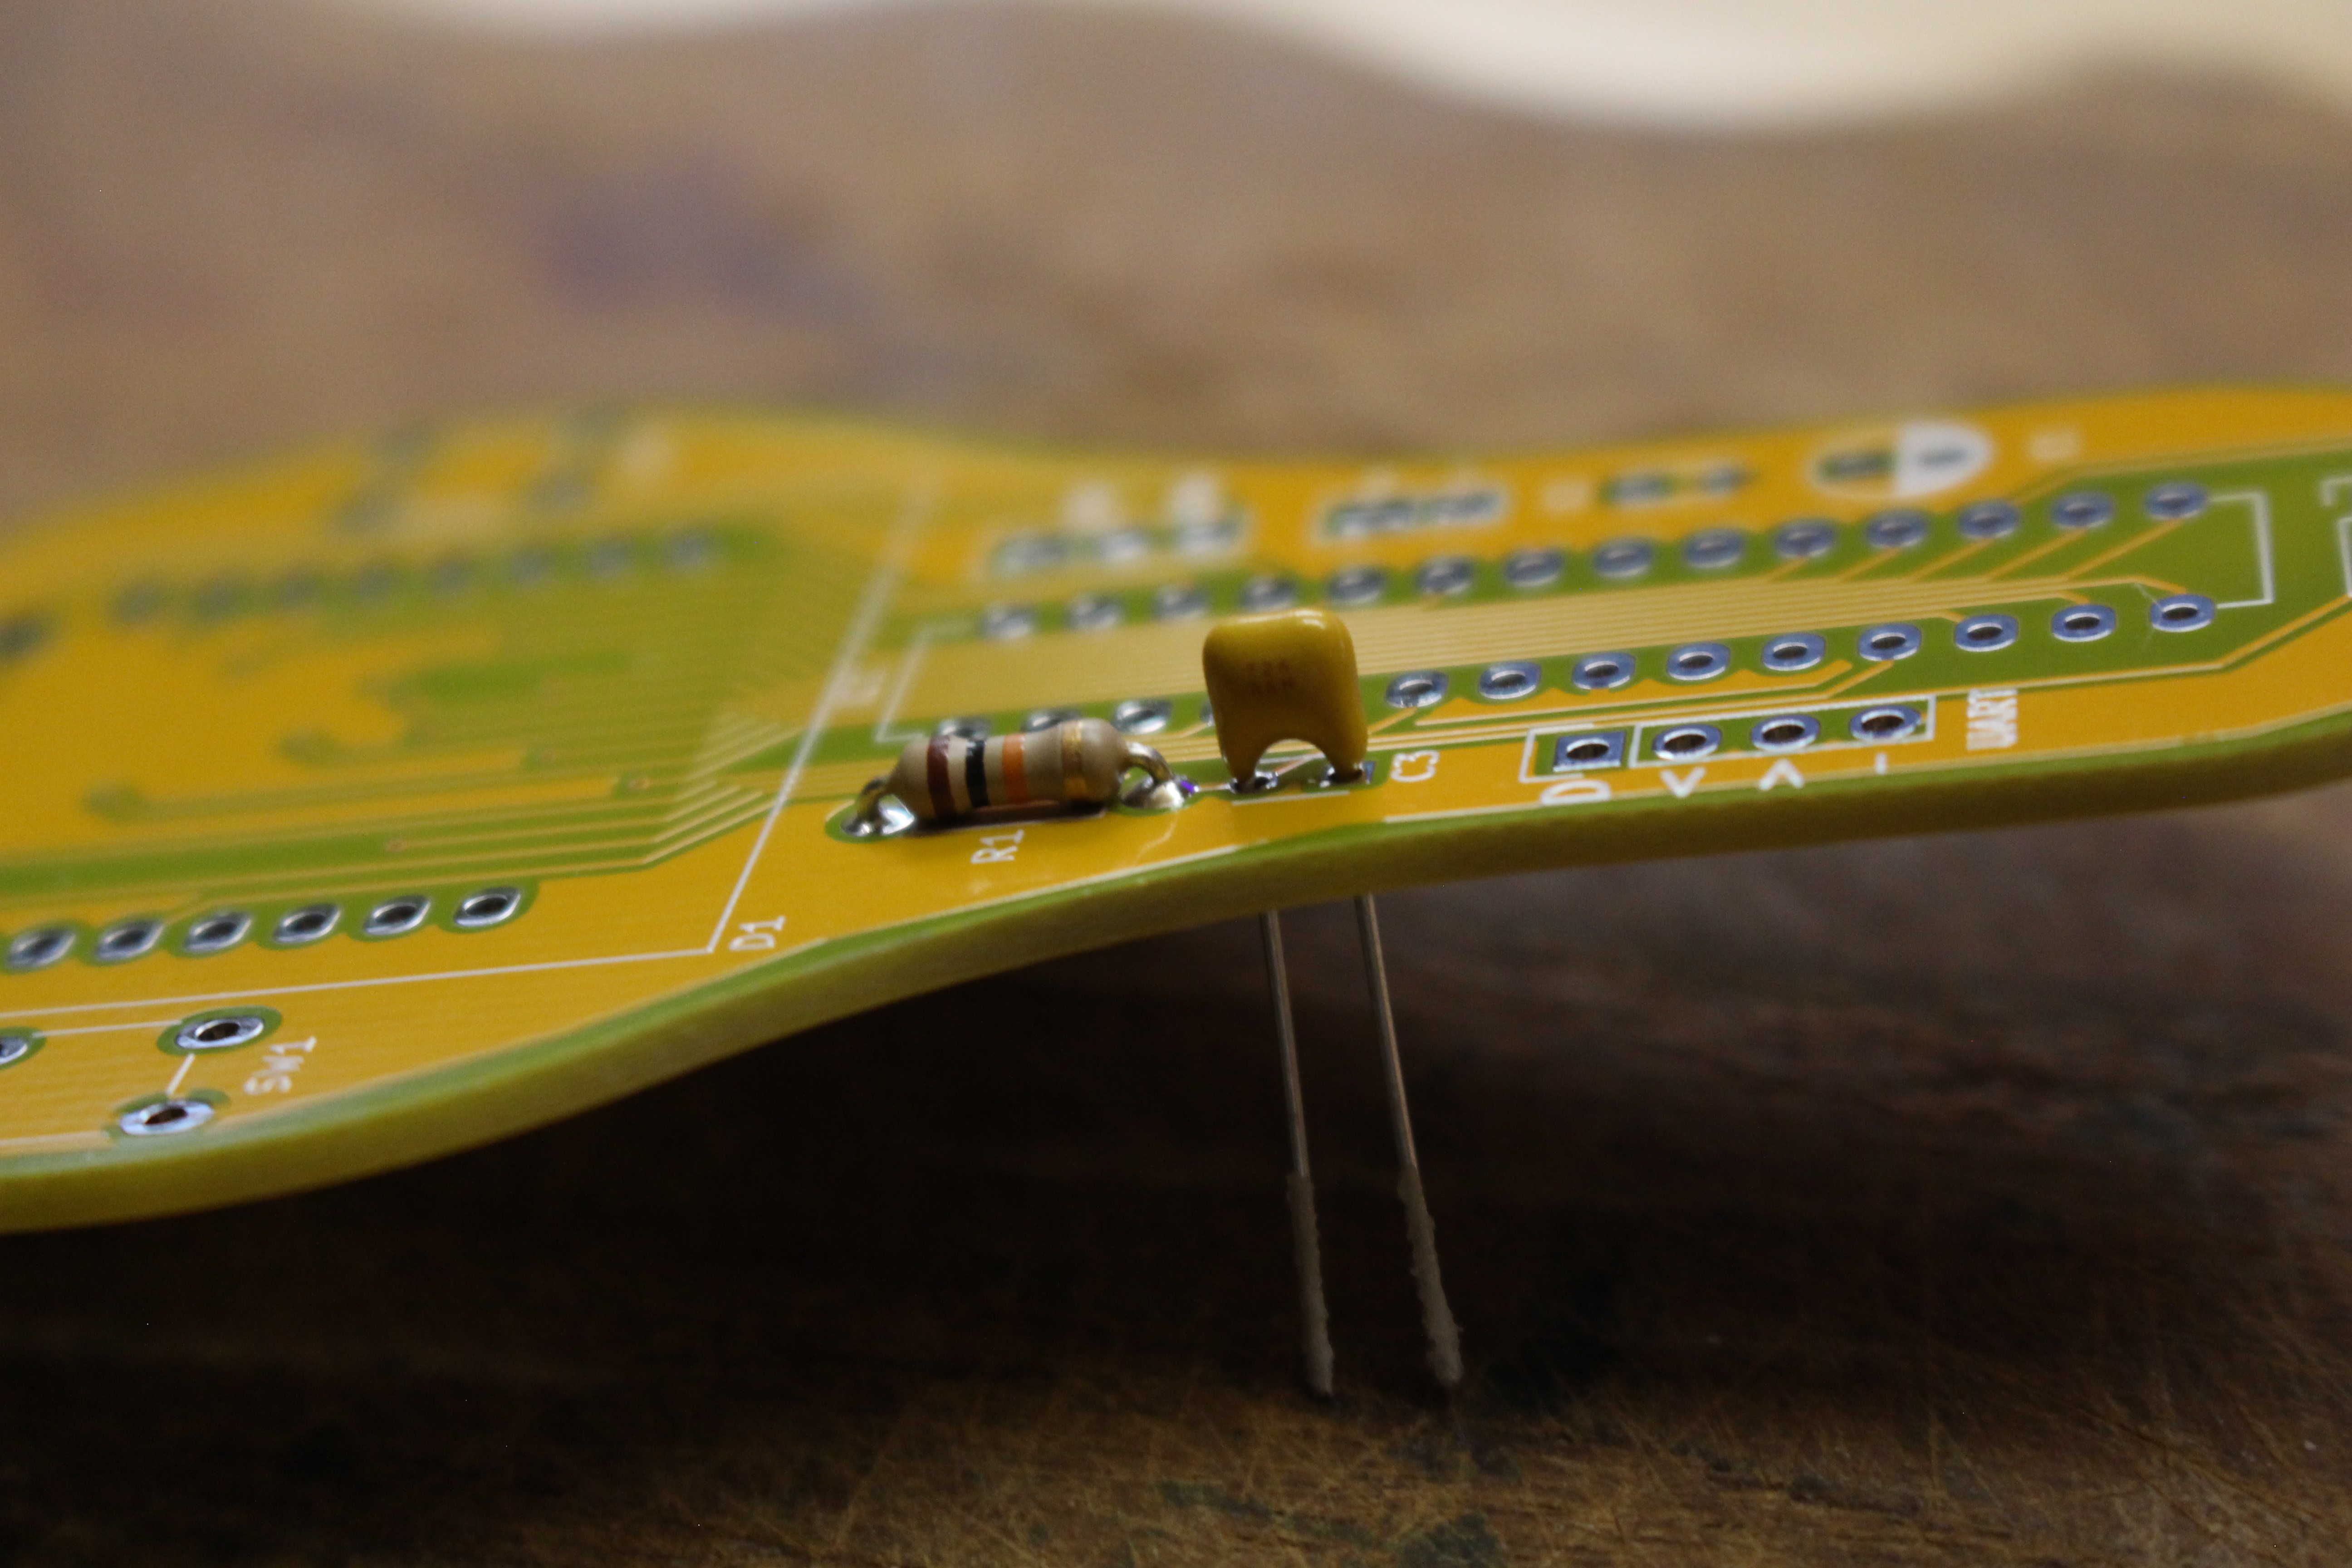
\includegraphics[width=\textwidth]{Bilder/IMG_5548.JPG}
	%\captionof{figure}{}
	%\label{fig:}
\end{minipage}
\begin{minipage}[b]{0.5\textwidth}
	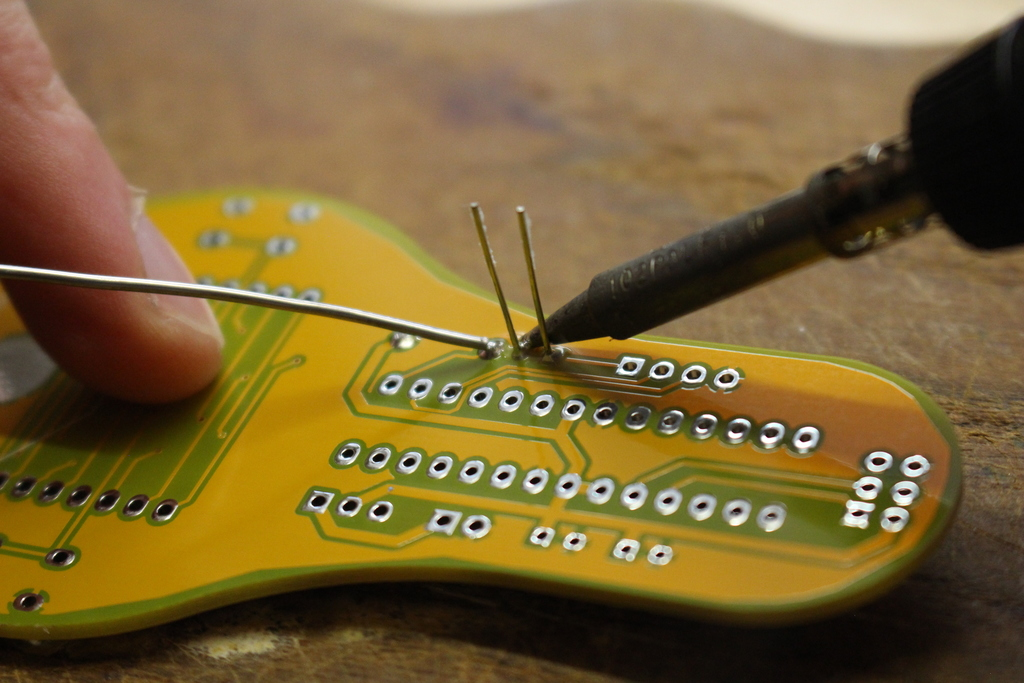
\includegraphics[width=\textwidth]{Bilder/IMG_5550.JPG}
	%\captionof{figure}{}
	%\label{fig:}
\end{minipage}

\vspace{0.5cm}

\begin{minipage}[b]{0.5\textwidth}
	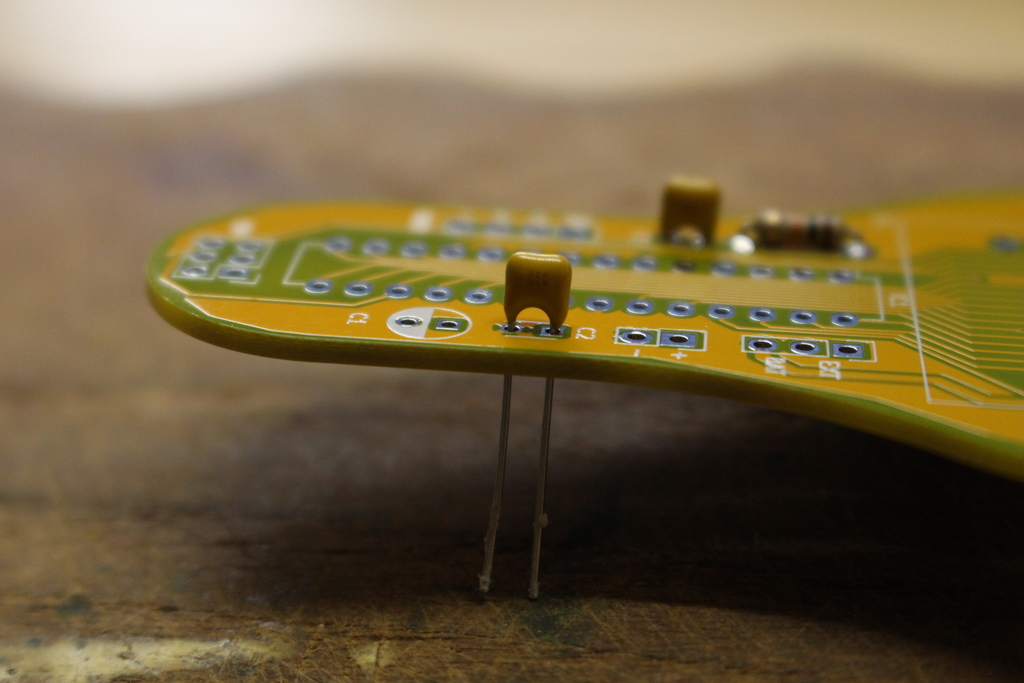
\includegraphics[width=\textwidth]{Bilder/IMG_5551.JPG}
	%\captionof{figure}{}
	%\label{fig:}
\end{minipage}
\begin{minipage}[b]{0.5\textwidth}
	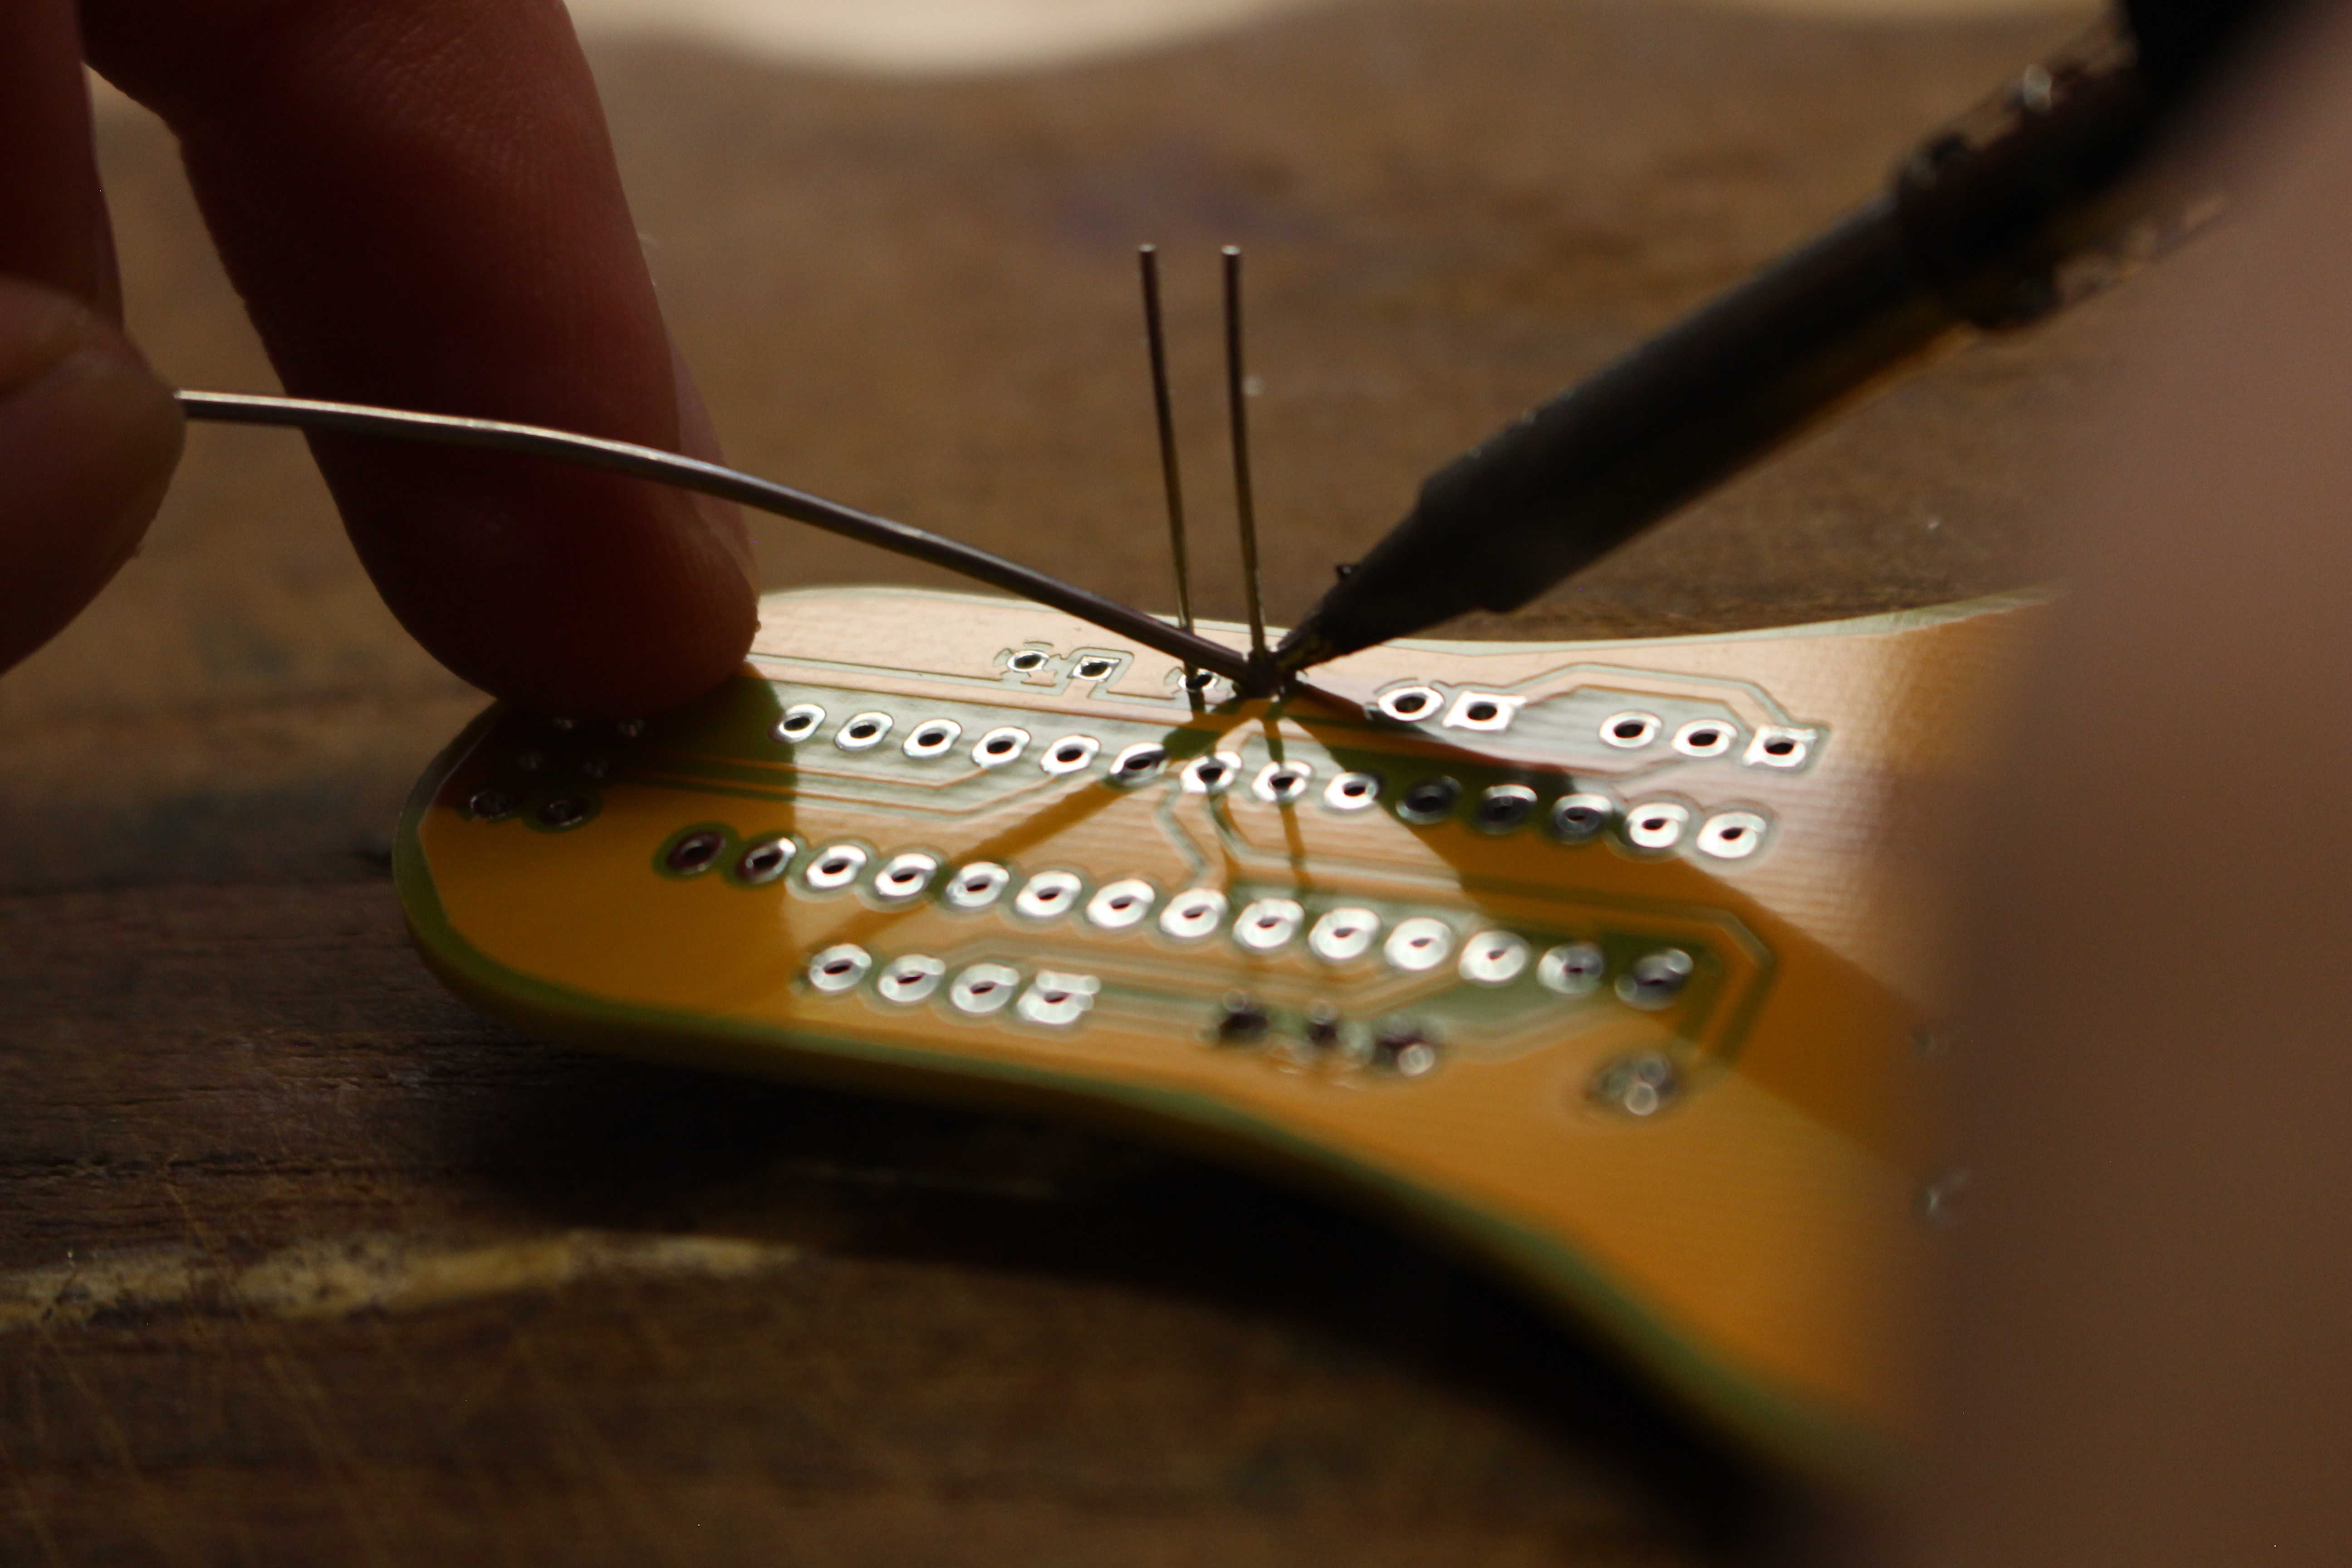
\includegraphics[width=\textwidth]{Bilder/IMG_5552.JPG}
	%\captionof{figure}{}
	%\label{fig:}
\end{minipage}

\subsection{Sockel für den Mikrocontroller}

Beim Sockel musst du ein bisschen aufpassen, dass er richtigherum eingelötet wird. Wenn er falschrum drin ist, ist das zwar kein Beinbruch, aber beim Löten von Platinen sollte man immer eine gewisse Sorgfalt walten lassen und auch auf solche Details achten.

Der Sockel hat eine halbrunde Einkerbung auf der einen Seite. Diese muss an der Seite auf der Platine platziert werden, wo die Pin 1 Markierung des Mikrocontrollers aufgedruckt ist. Die Markierung ist ein kleiner Querstrich links unterhalb der IC1 Beschriftung.

Wenn der Sockel richtig sitzt, kannst du die Platine wieder umdrehen und die Platine mit dem Sockel gegen das Brett drücken. Dann verlötest du am besten einen Pin und prüfst noch einmal, ob der Sockel auch wirklich richtig auf der Platine aufsitzt. Ist alles Okay, kannst du alle anderen Pins in einem Rutsch festlöten.

\vspace{1cm}

\begin{minipage}[b]{0.5\textwidth}
	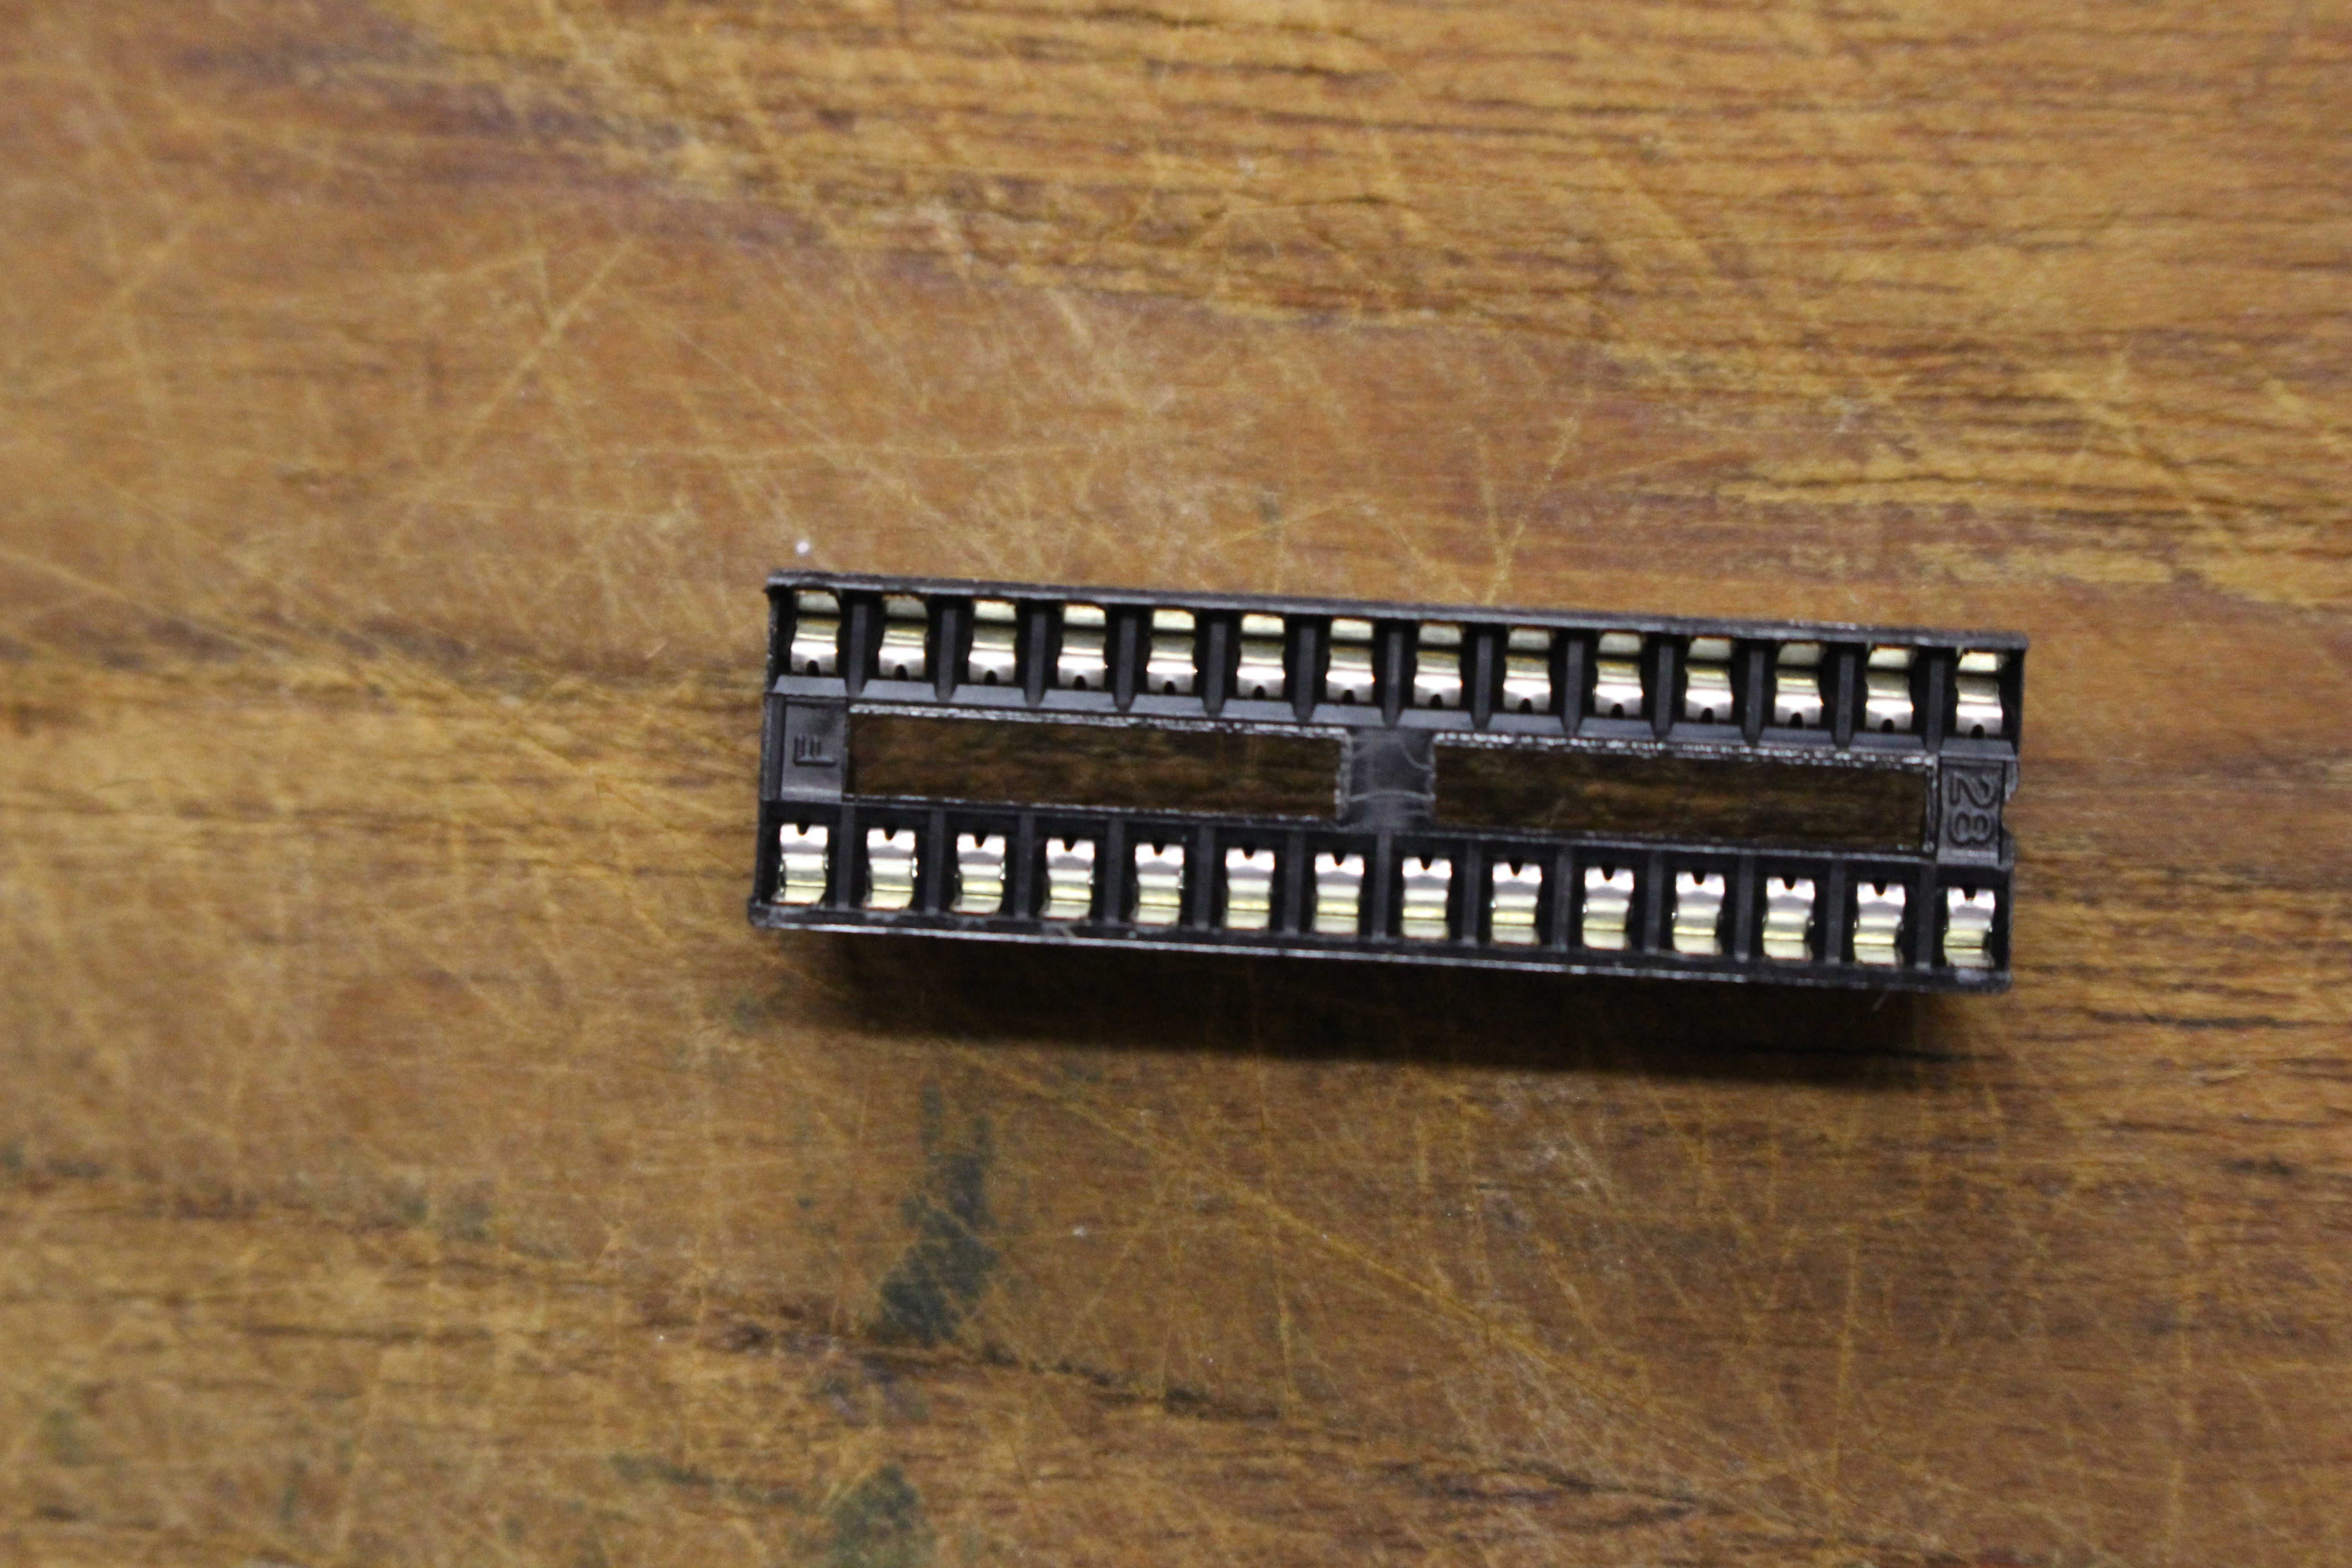
\includegraphics[width=\textwidth]{Bilder/IMG_5553.JPG}
	%\captionof{figure}{}
	%\label{fig:}
\end{minipage}
\begin{minipage}[b]{0.5\textwidth}
	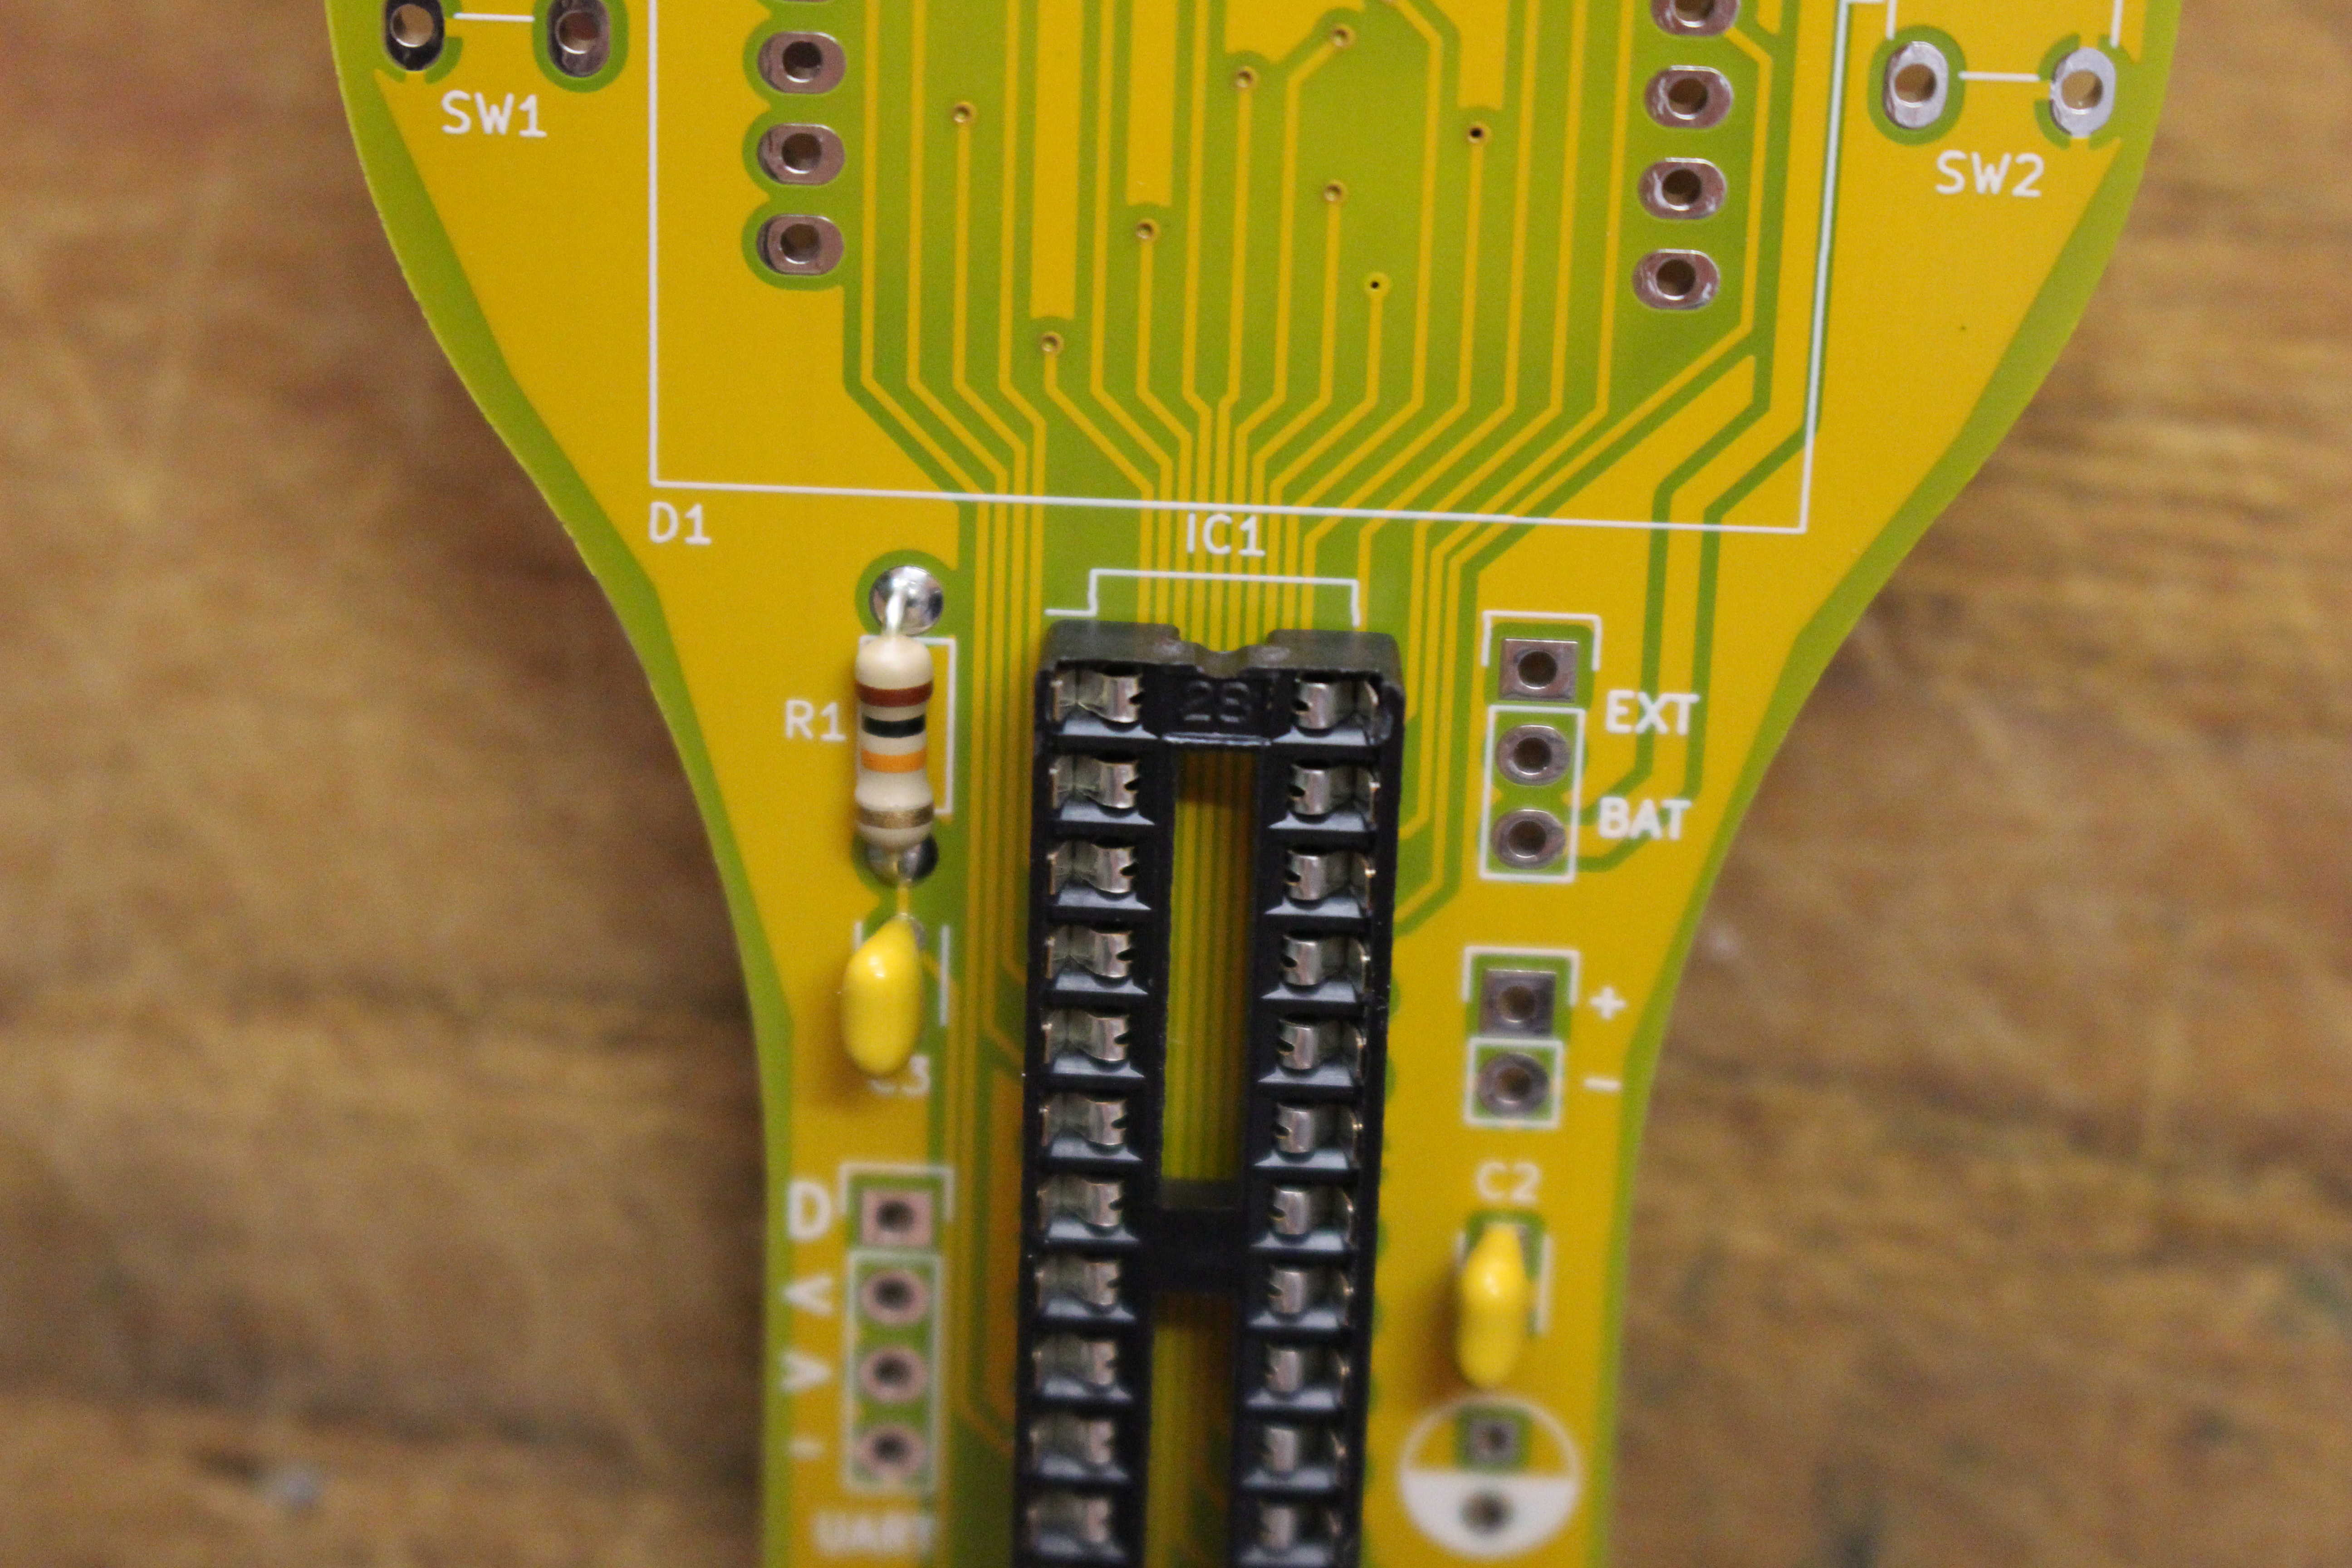
\includegraphics[width=\textwidth]{Bilder/IMG_5554.JPG}
	%\captionof{figure}{}
	%\label{fig:}
\end{minipage}

\vspace{0.5cm}

\begin{minipage}[b]{0.5\textwidth}
	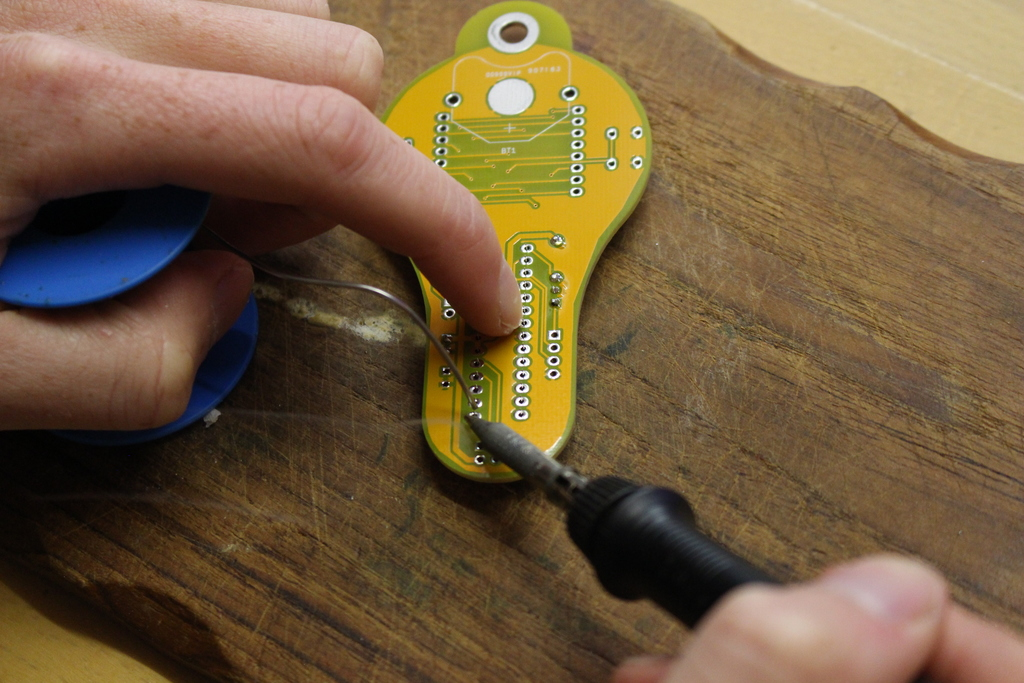
\includegraphics[width=\textwidth]{Bilder/IMG_5555.JPG}
	%\captionof{figure}{}
	%\label{fig:}
\end{minipage}
\begin{minipage}[b]{0.5\textwidth}
	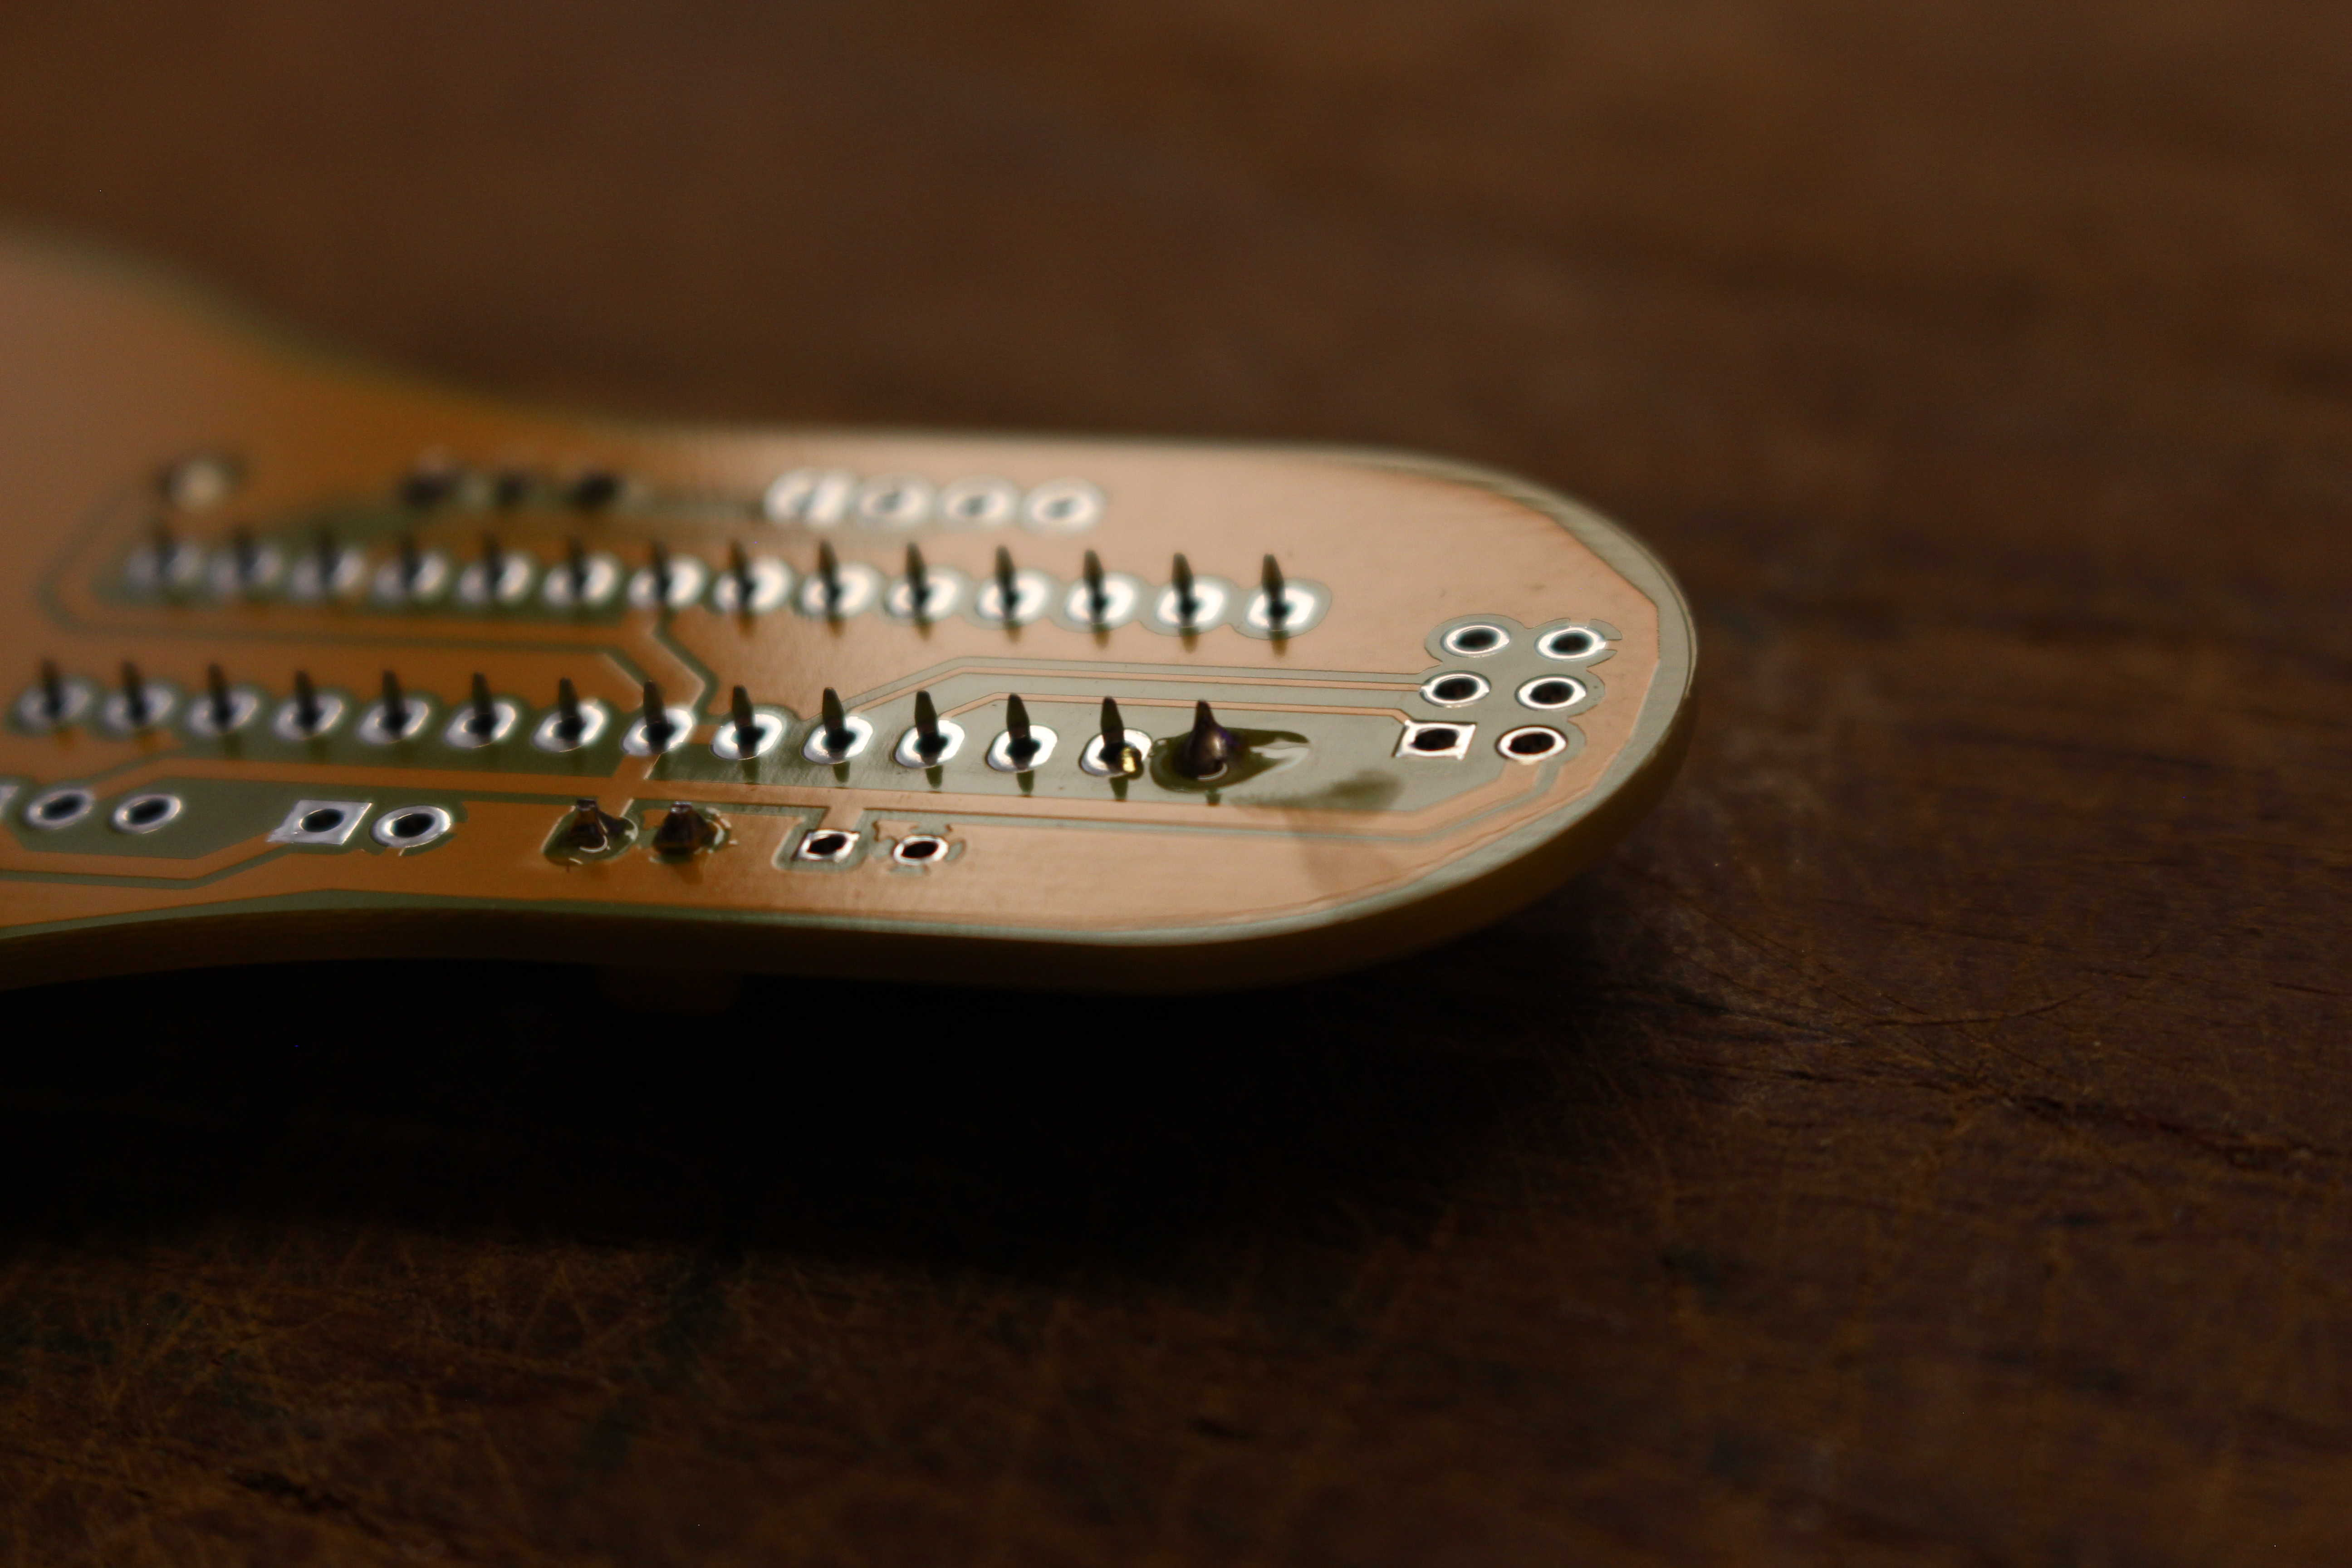
\includegraphics[width=\textwidth]{Bilder/IMG_5558.JPG}
	%\captionof{figure}{}
	%\label{fig:}
\end{minipage}

\vspace{0.5cm}

\begin{minipage}[b]{0.5\textwidth}
	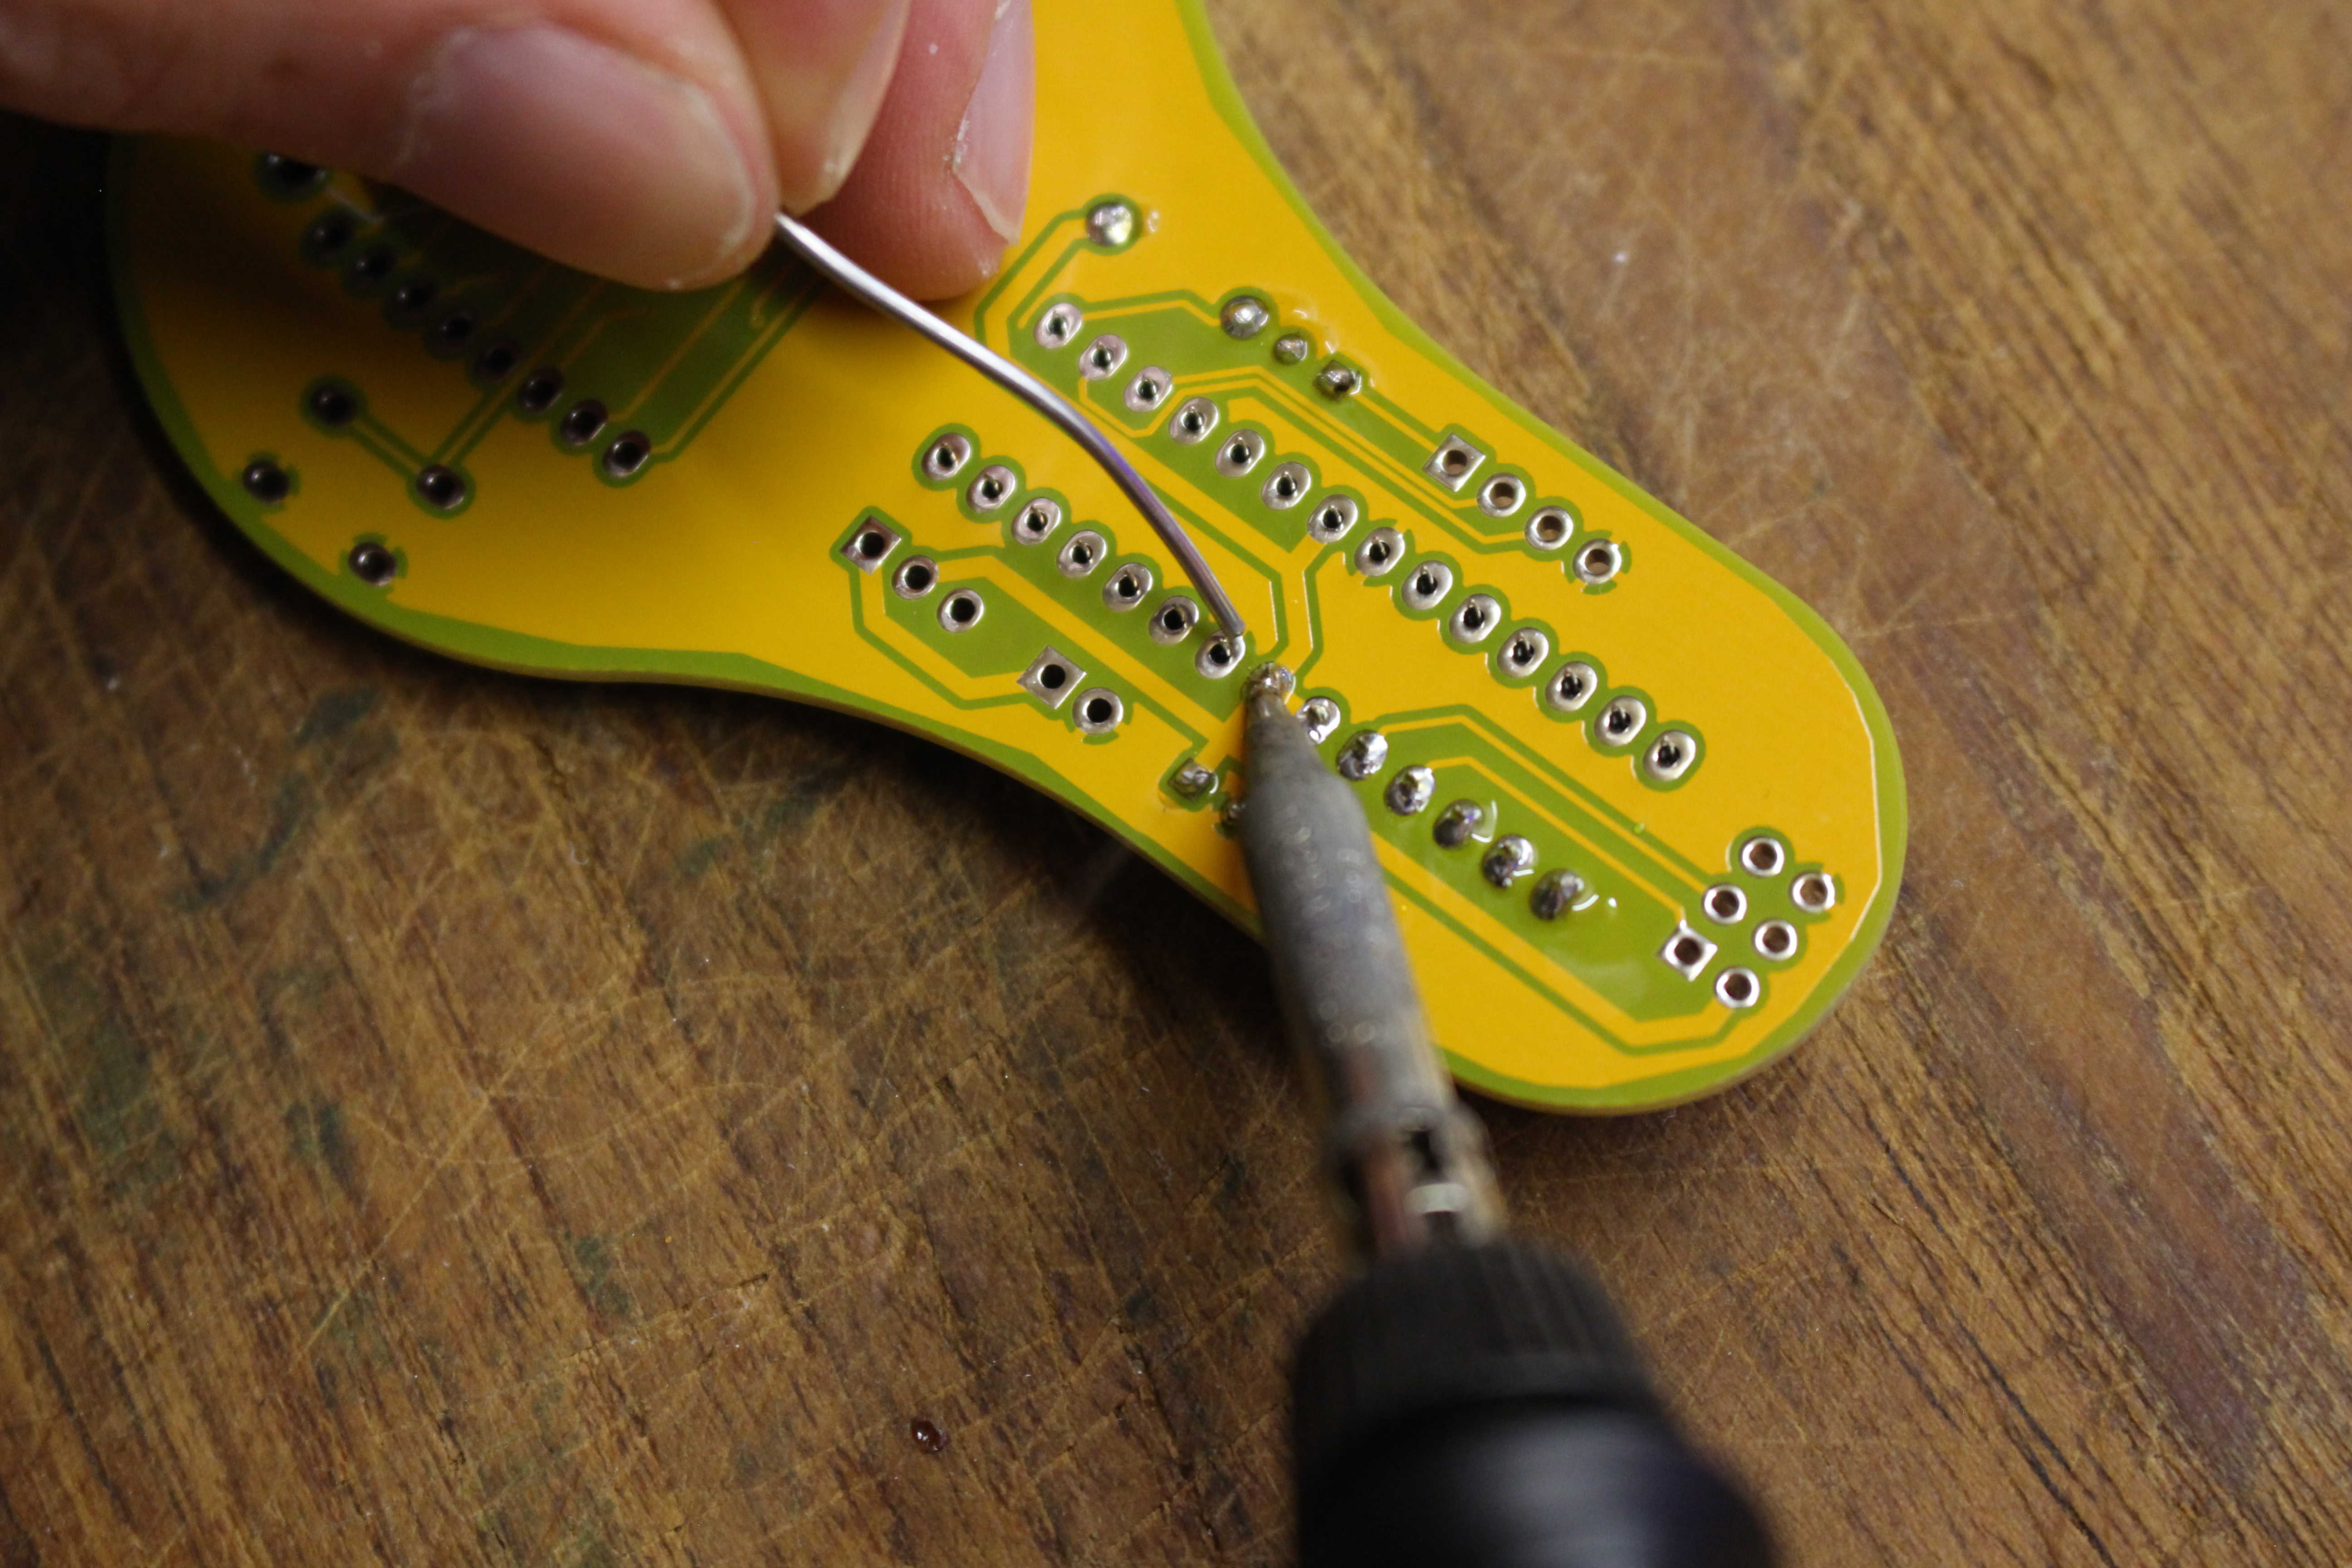
\includegraphics[width=\textwidth]{Bilder/IMG_5559.JPG}
	%\captionof{figure}{}
	%\label{fig:}
\end{minipage}
\begin{minipage}[b]{0.5\textwidth}
	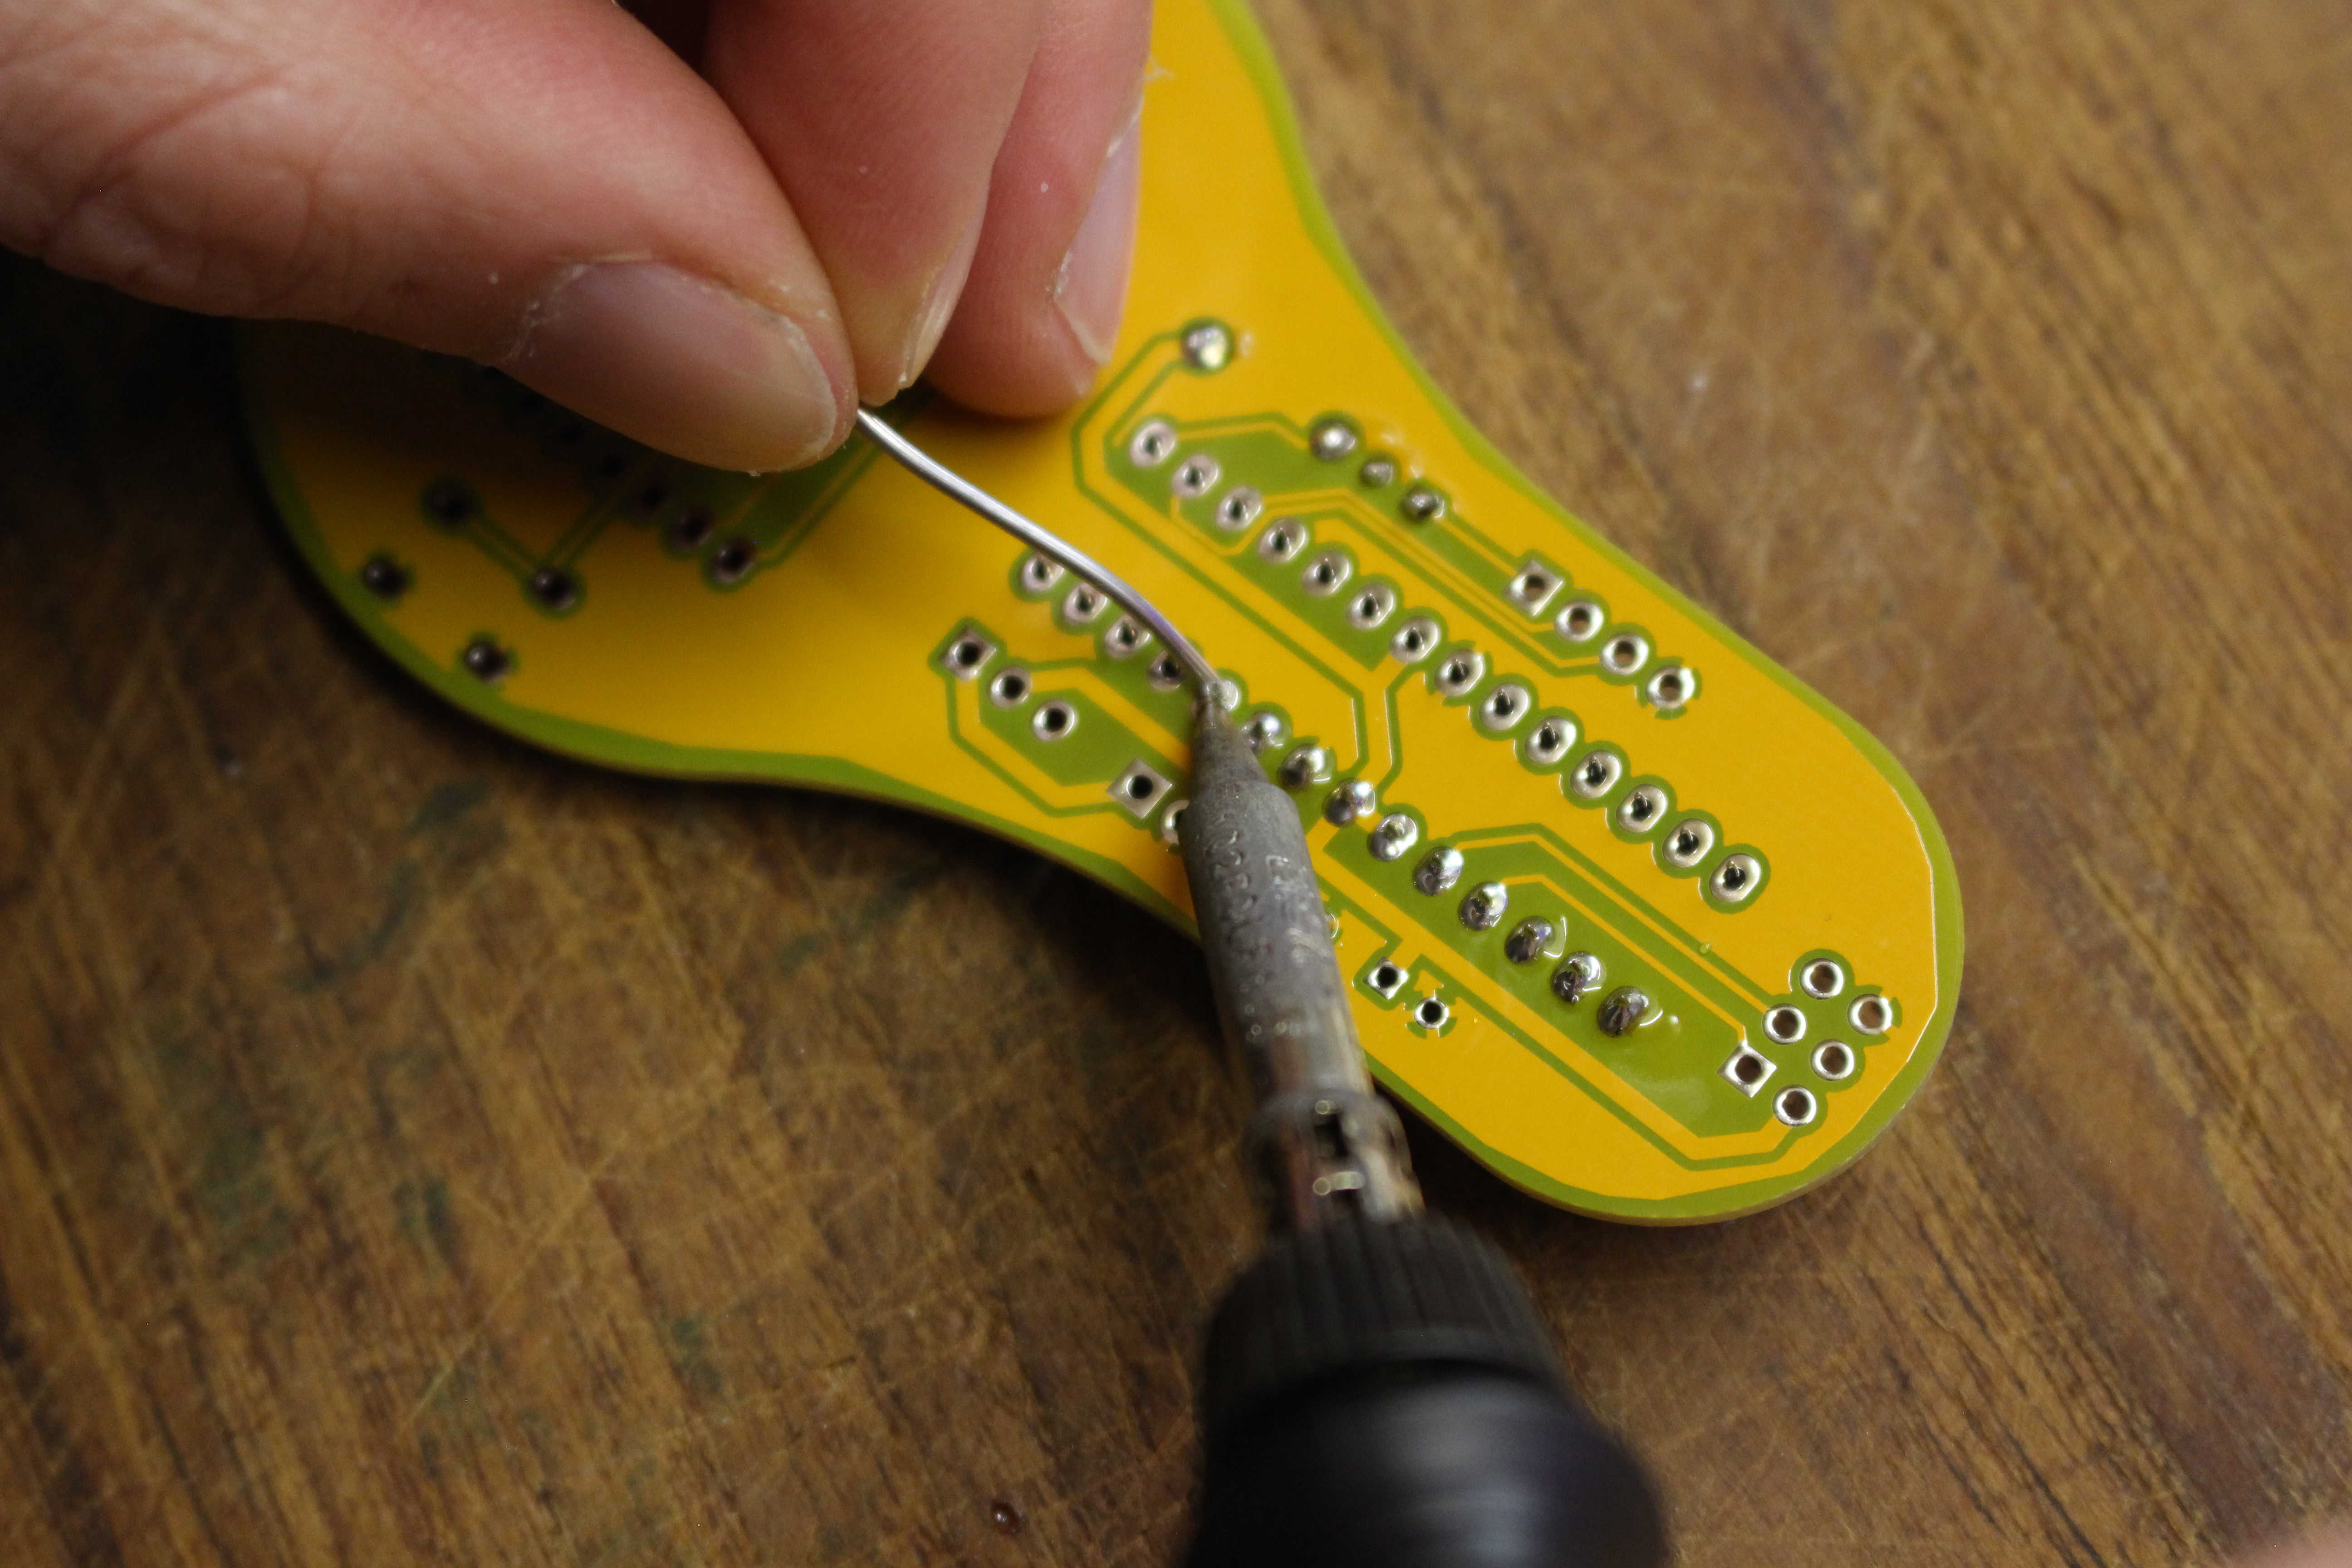
\includegraphics[width=\textwidth]{Bilder/IMG_5560.JPG}
	%\captionof{figure}{}
	%\label{fig:}
\end{minipage}

\subsection{Knopfzellenhalter - BT1}

Bevor du den Knopfzellenhalter anlöten darfst, musst du die große runde silberne Fläche mit Lötzinn versehen. Dazu lässt du ein kleines bisschen Lötzinn auf der Fläche schmelzen und verteilst sie mit dem Lötkolben, indem du den Lötkolben kreisförmig über die Fläche bewegst.

Das musst du tun, damit die Knopfzelle später einen ordentlichen Kontakt zur Platinenoberfläche hat.

Wenn du den Knopfzellenhalter festlötest, wirst du merken, dass das nicht so einfach geht, wie bei den Pins vorher. Das liegt daran, dass das viele Metall des Halters länger braucht um warm zu werden. Hier musst du also nur ein bisschen Geduld haben, bis das Lötzinn ordentlich fließt.

\vspace{1cm}

\begin{minipage}[b]{0.5\textwidth}
	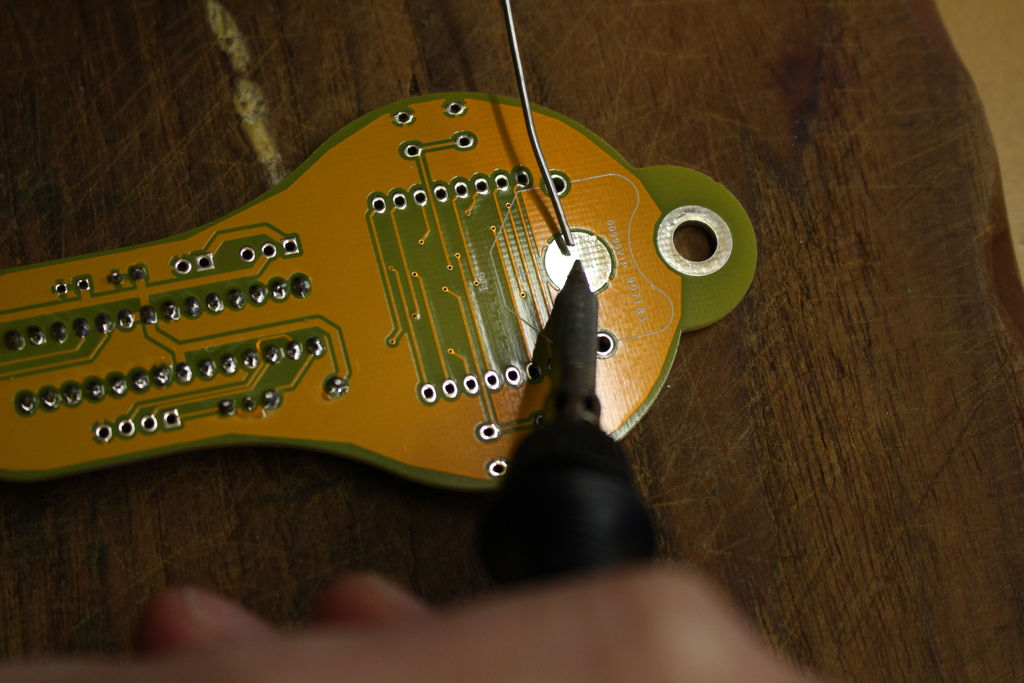
\includegraphics[width=\textwidth]{Bilder/IMG_5561.JPG}
	%\captionof{figure}{}
	%\label{fig:}
\end{minipage}
\begin{minipage}[b]{0.5\textwidth}
	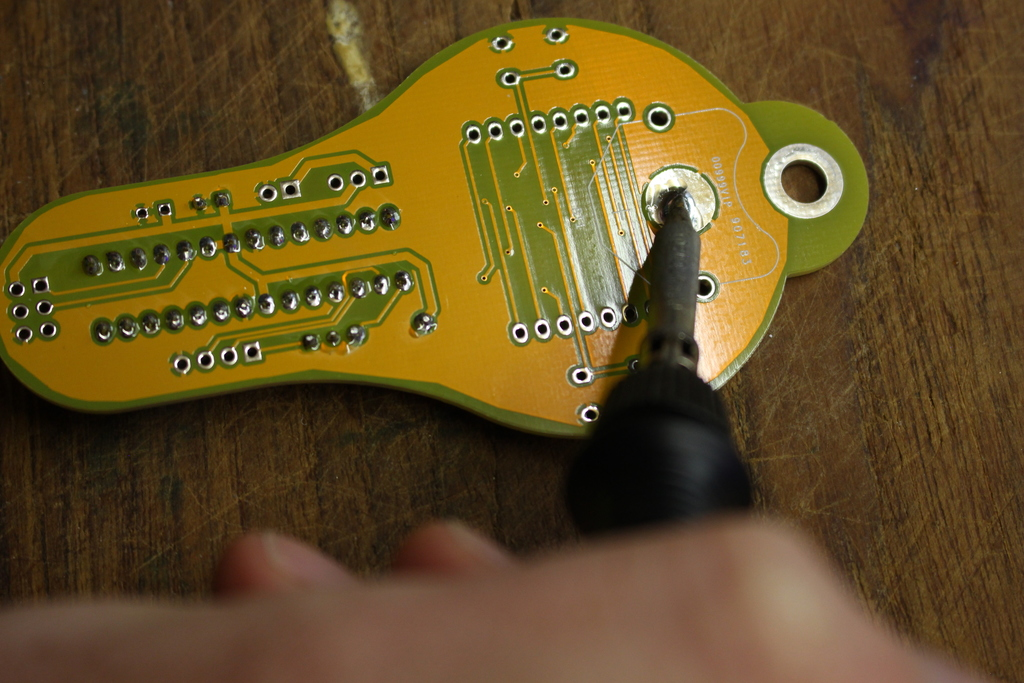
\includegraphics[width=\textwidth]{Bilder/IMG_5562.JPG}
	%\captionof{figure}{}
	%\label{fig:}
\end{minipage}

\vspace{0.5cm}

\begin{minipage}[b]{0.5\textwidth}
	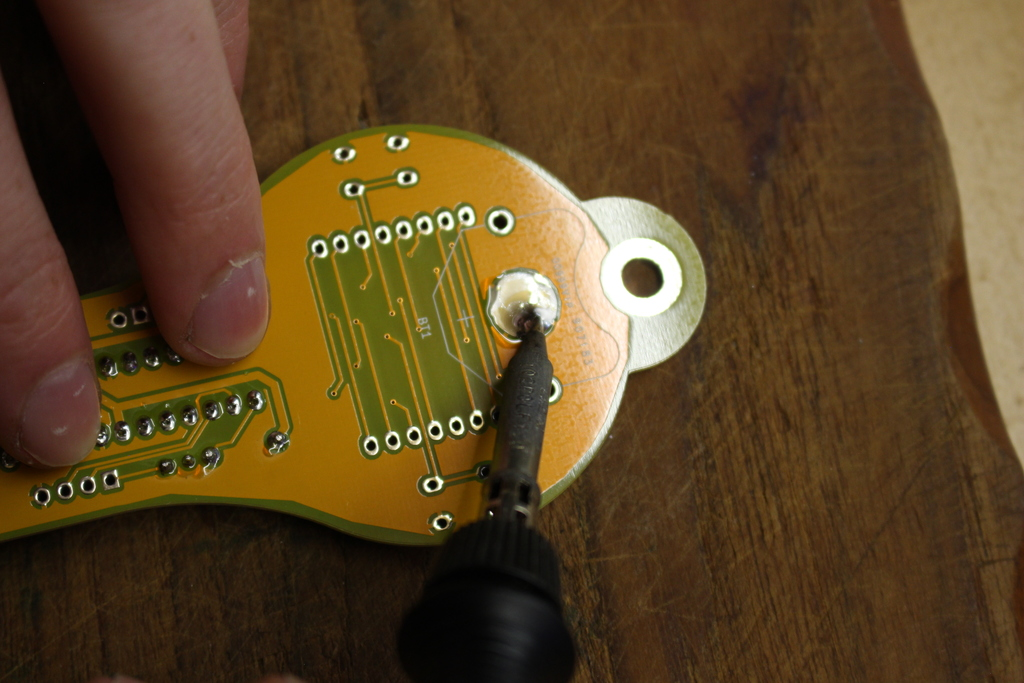
\includegraphics[width=\textwidth]{Bilder/IMG_5563.JPG}
	%\captionof{figure}{}
	%\label{fig:}
\end{minipage}
\begin{minipage}[b]{0.5\textwidth}
	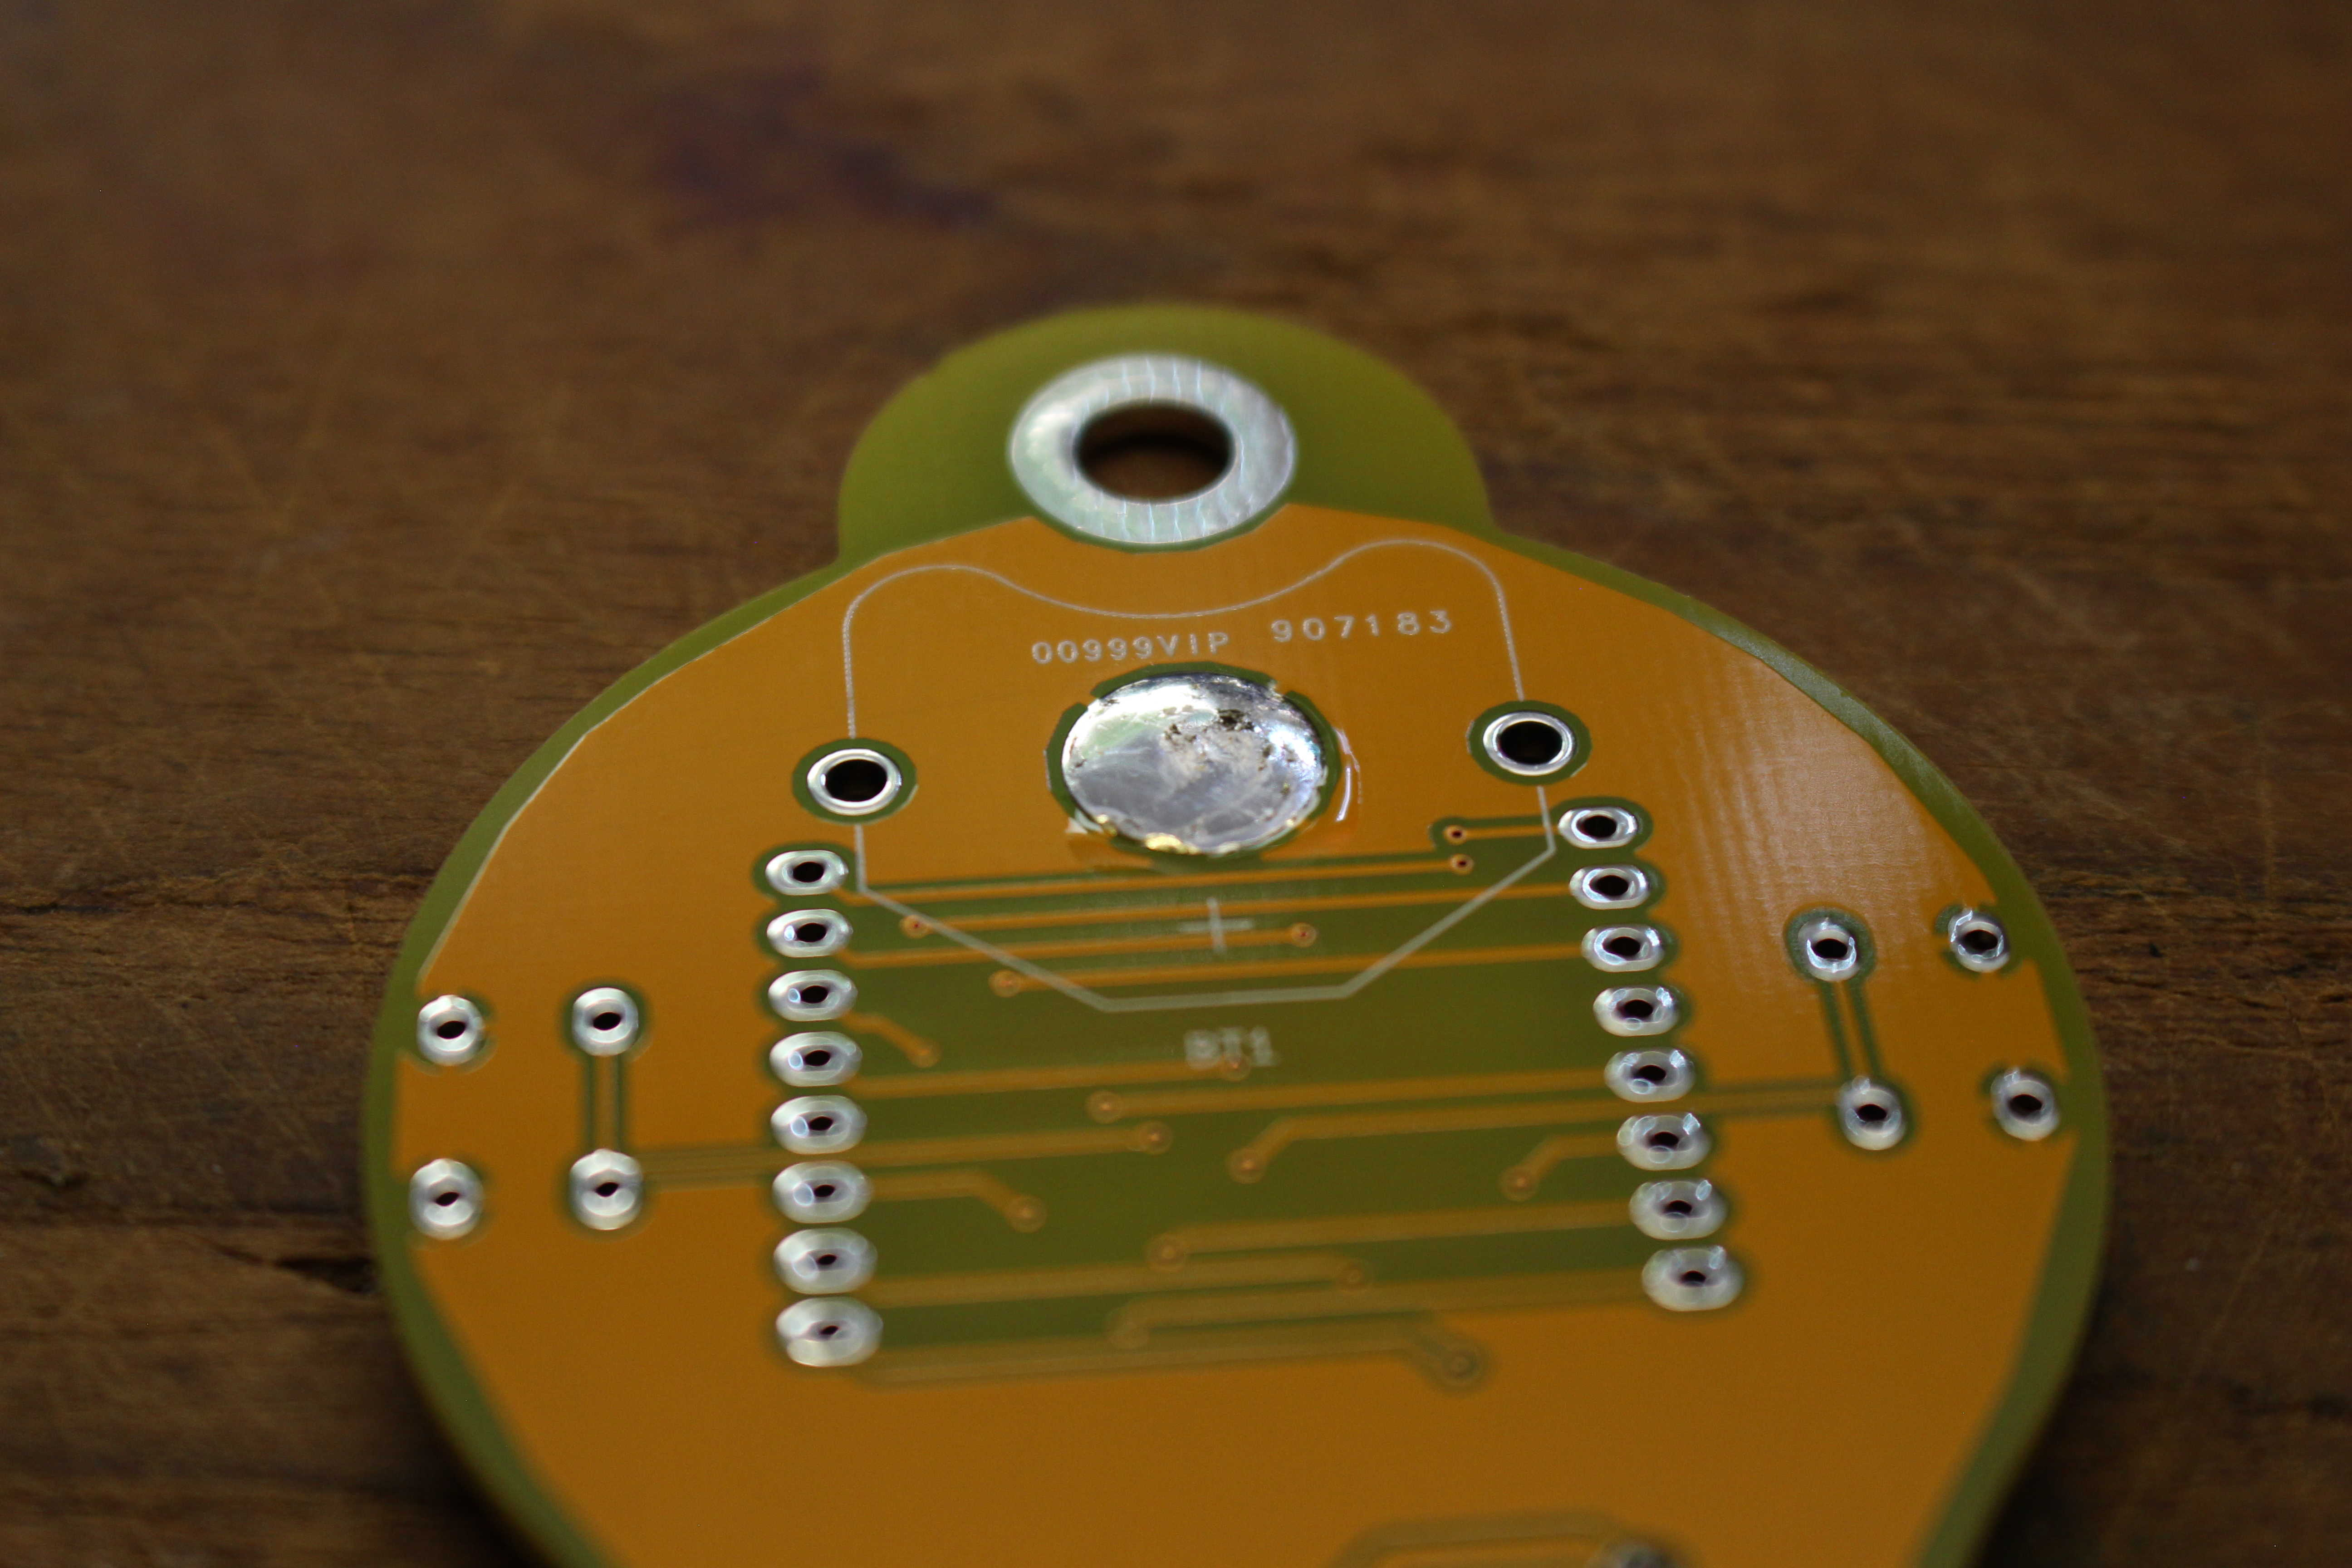
\includegraphics[width=\textwidth]{Bilder/IMG_5564.JPG}
	%\captionof{figure}{}
	%\label{fig:}
\end{minipage}

\vspace{0.5cm}

\begin{minipage}[b]{0.5\textwidth}
	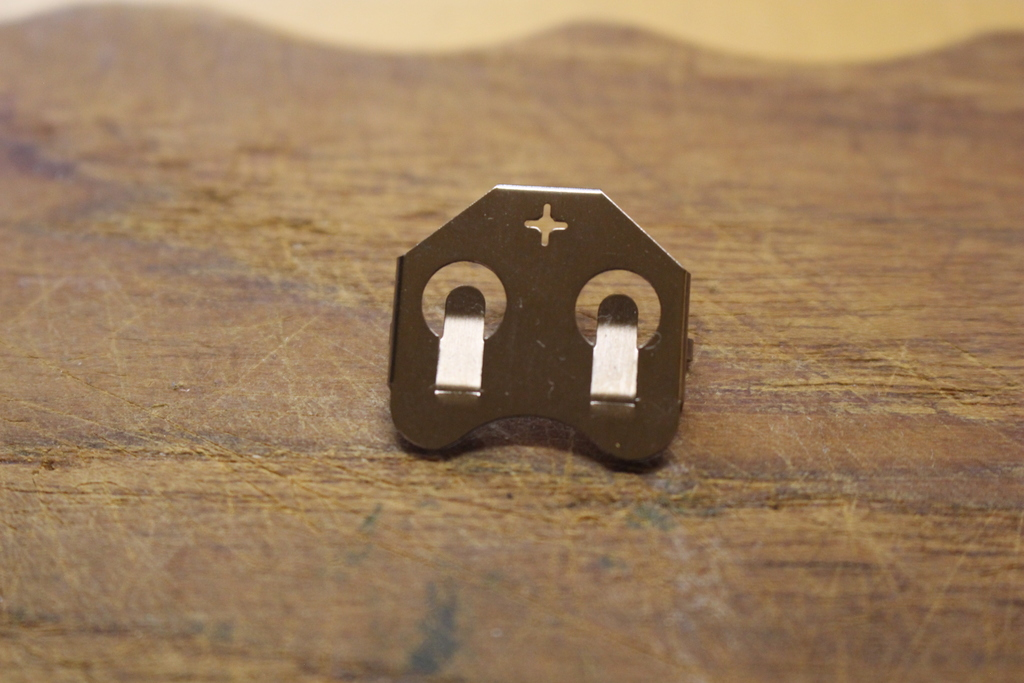
\includegraphics[width=\textwidth]{Bilder/IMG_5565.JPG}
	%\captionof{figure}{}
	%\label{fig:}
\end{minipage}
\begin{minipage}[b]{0.5\textwidth}
	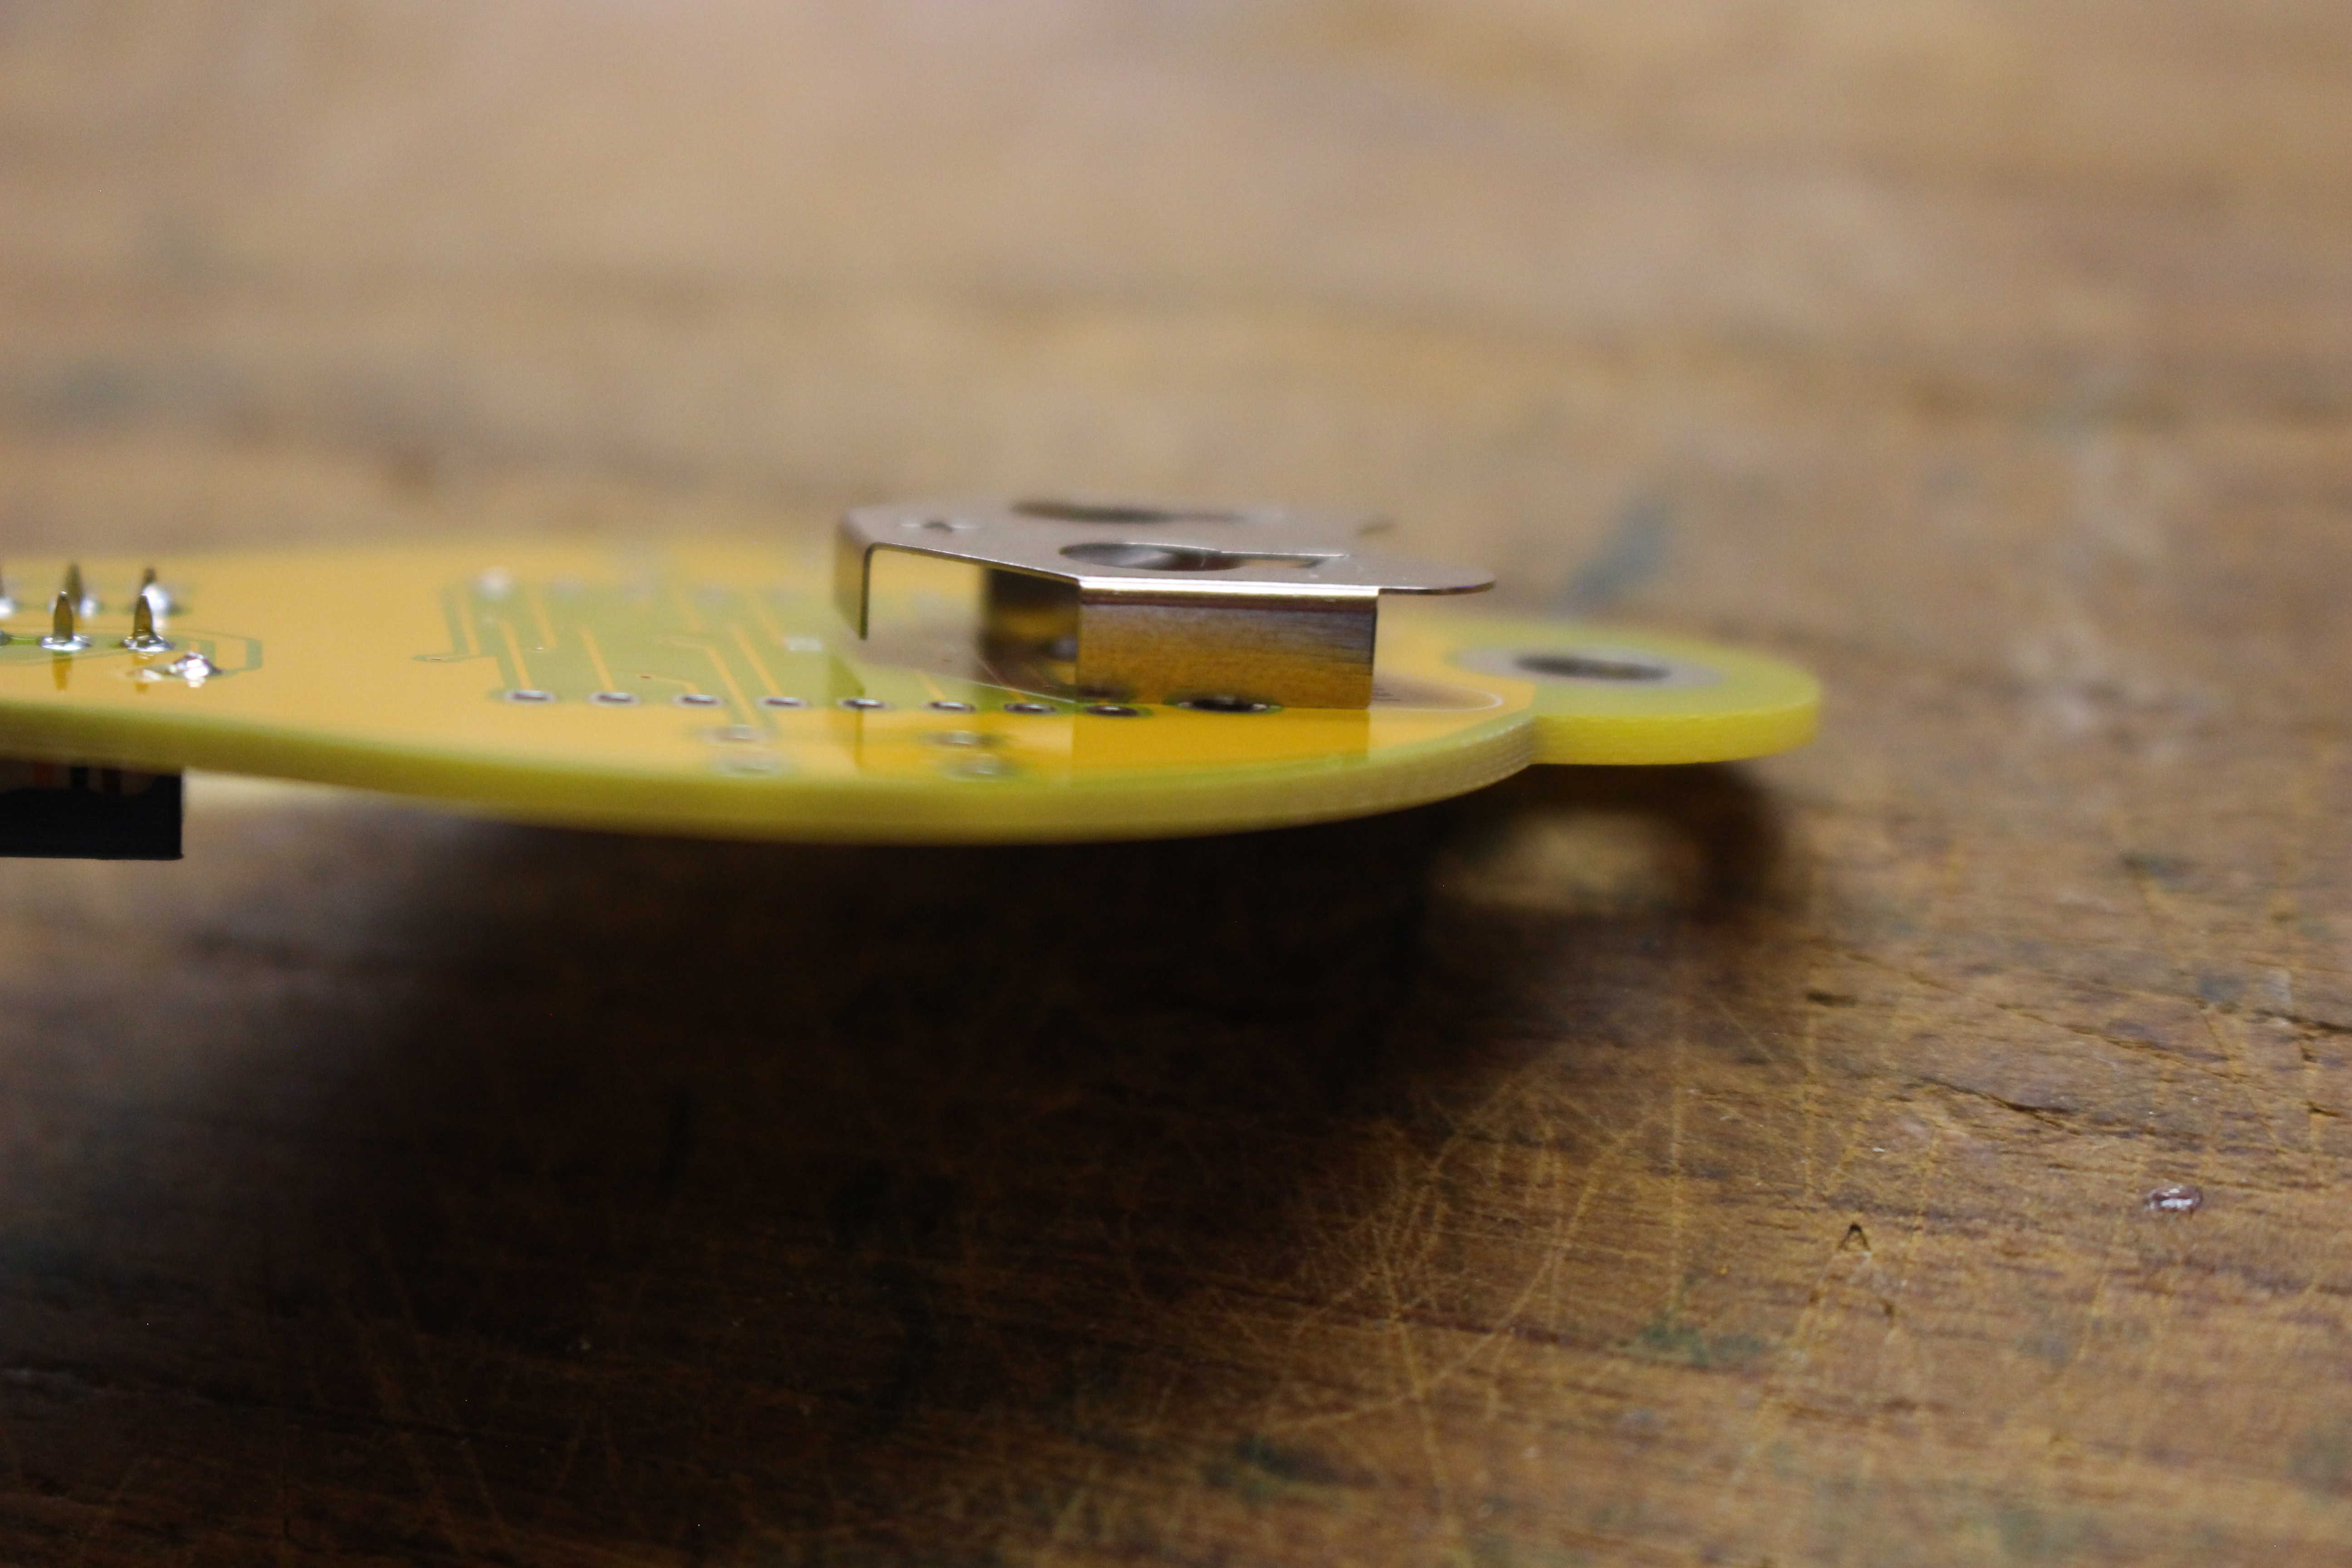
\includegraphics[width=\textwidth]{Bilder/IMG_5566.JPG}
	%\captionof{figure}{}
	%\label{fig:}
\end{minipage}

\vspace{0.5cm}

\begin{minipage}[b]{0.5\textwidth}
	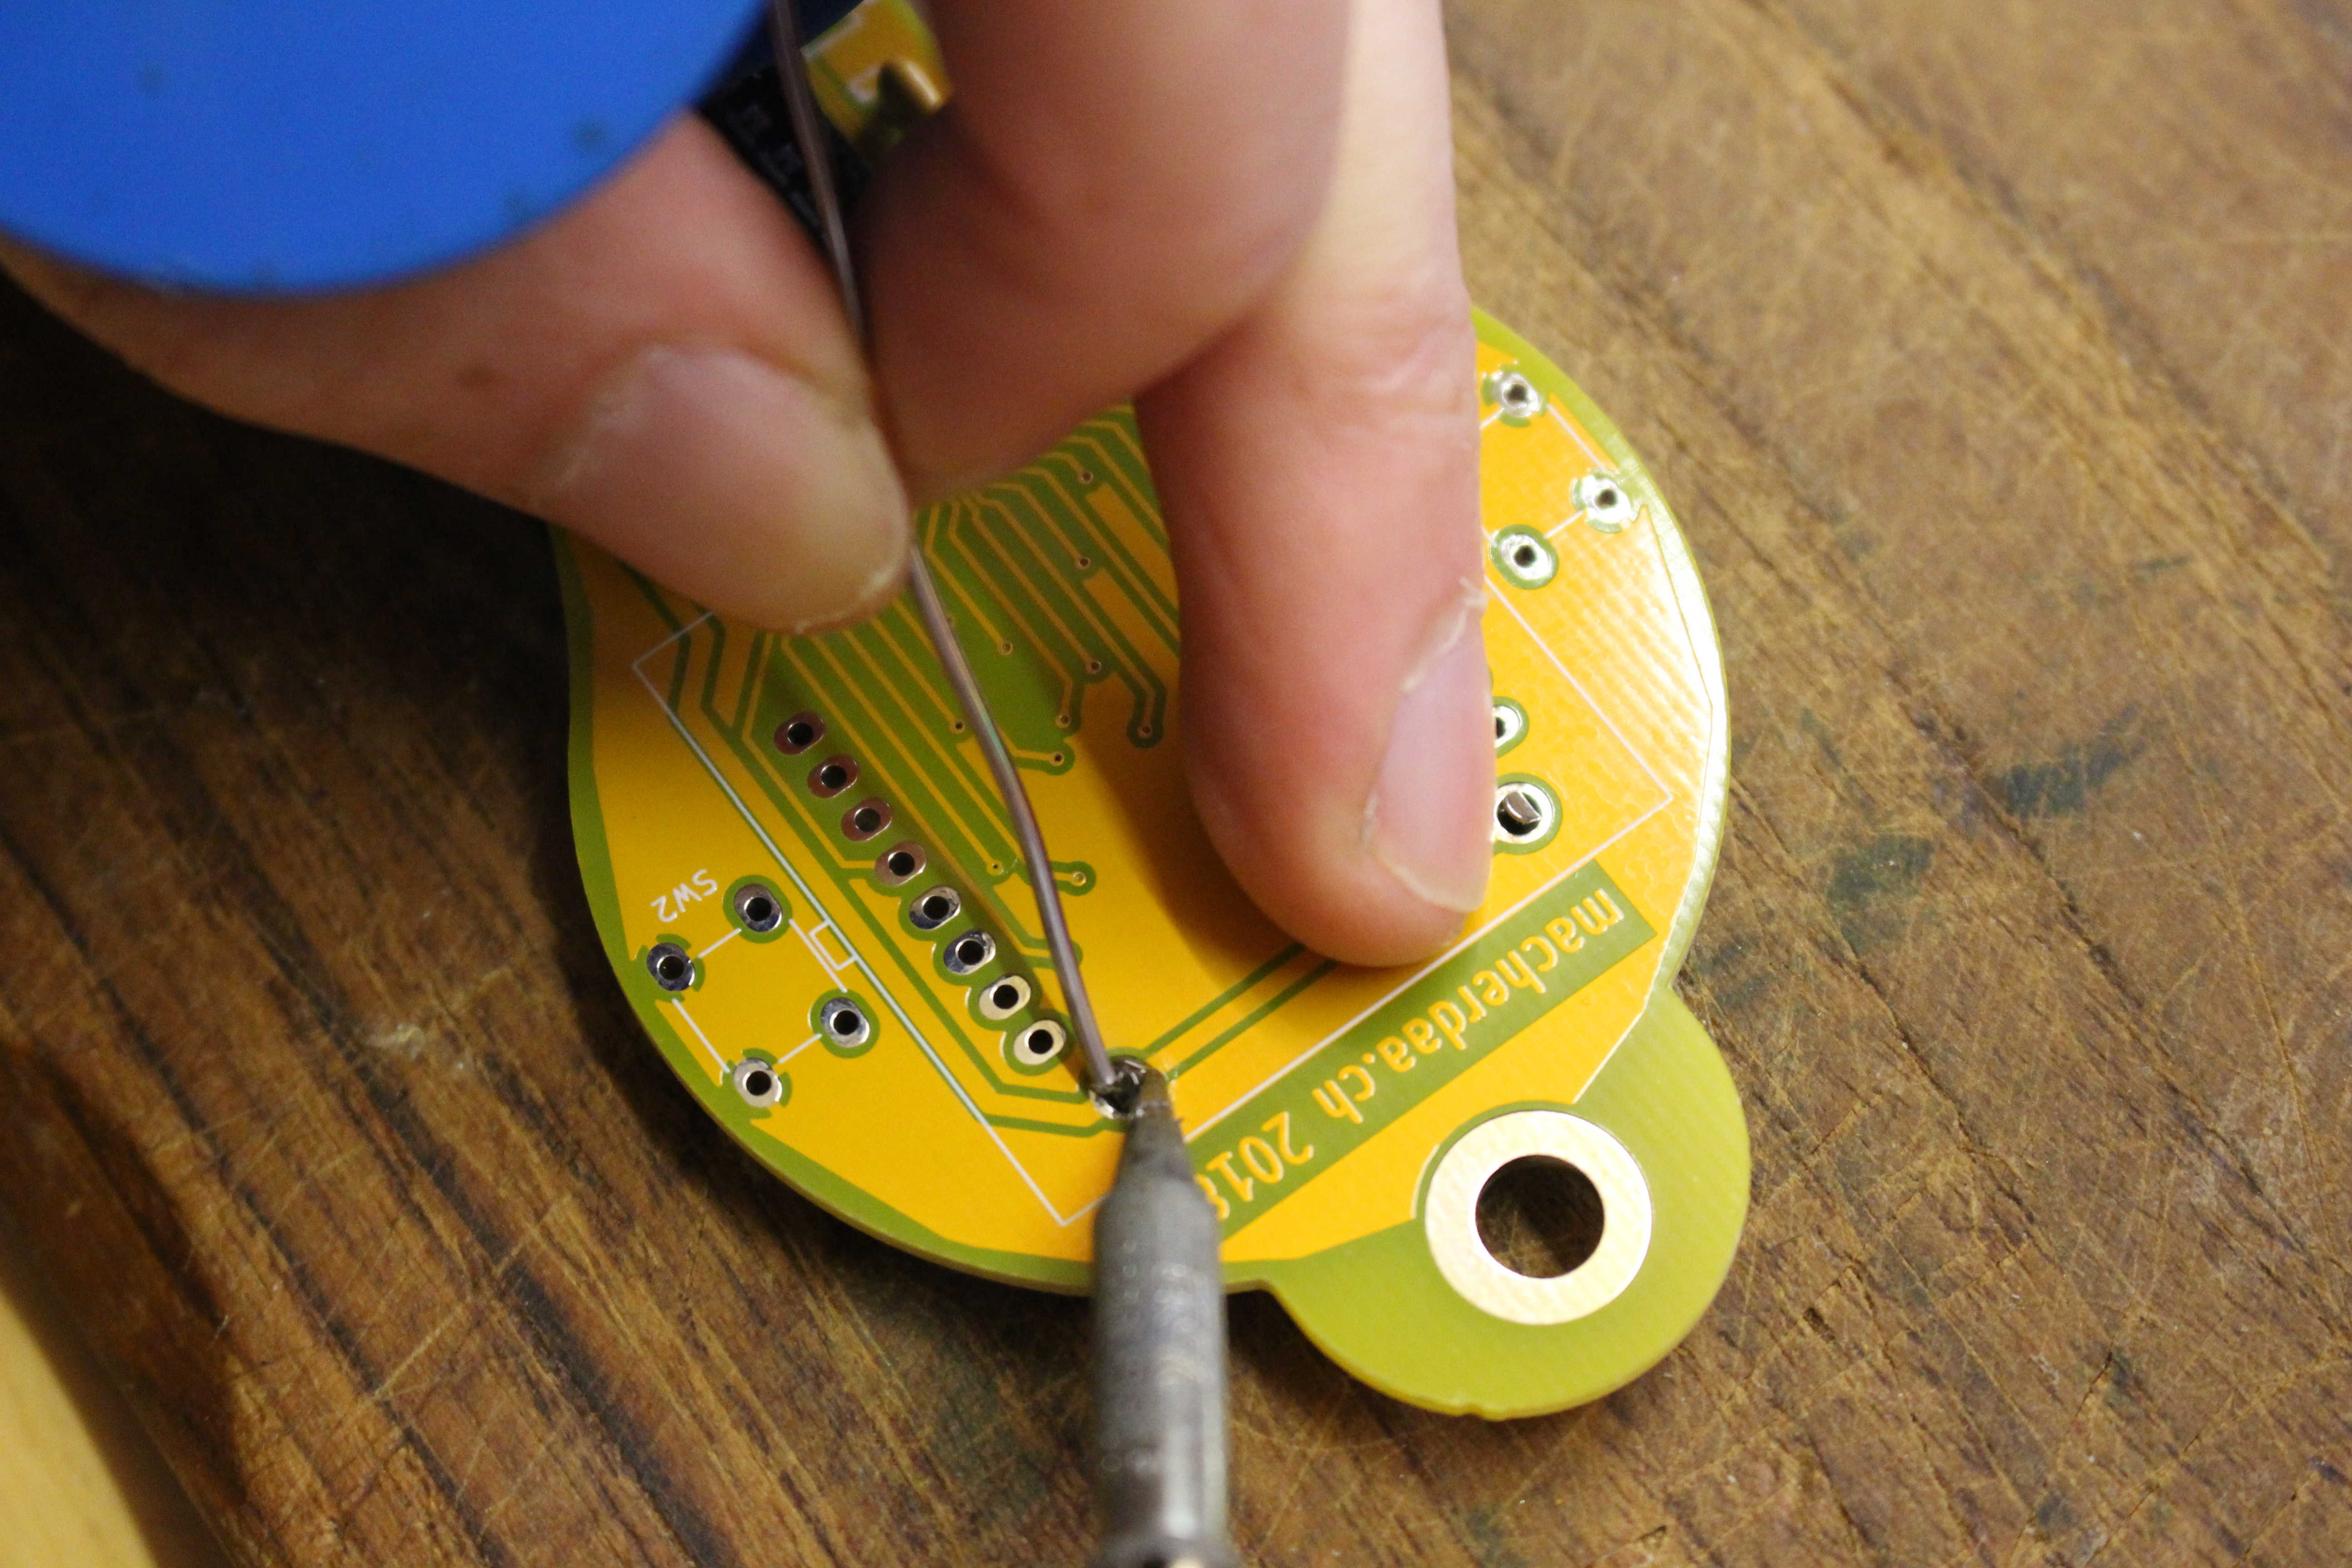
\includegraphics[width=\textwidth]{Bilder/IMG_5569.JPG}
	%\captionof{figure}{}
	%\label{fig:}
\end{minipage}
\begin{minipage}[b]{0.5\textwidth}
	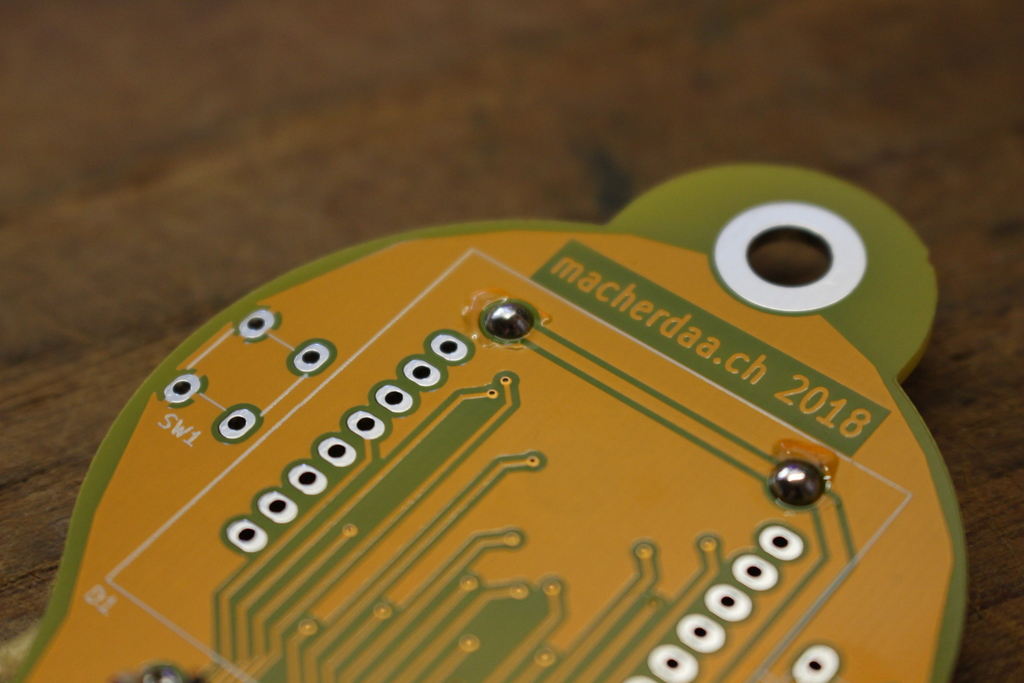
\includegraphics[width=\textwidth]{Bilder/IMG_5573.JPG}
	%\captionof{figure}{}
	%\label{fig:}
\end{minipage}

\subsection{LED-Matrix - D1}

Im Gegensatz zum Mikrocontrollersockel verzeiht dir die LED-Matrix nicht, wenn du sie falsch herum auflötest. Deshalb musst du auf die Markierung auf der Matrix achten. Das ist ein kleiner Nippel auf der Seite, auf der auch die Beschriftung der Matrix aufgedruckt ist. Die zugehörige Markierung auf der Platine ist ein kleines Rechteck am rechten Rand zwischen dem Bestückungsdruck für die Matrix und dem Taster SW2.

Beim Löten machst du das am besten so wie beim Mikrocontrollersockel. Du lötest erst einen Pin fest, prüfst ob alles richtig sitzt und dann lötest du alle anderen Pins.

\vspace{1cm}

\begin{minipage}[b]{0.5\textwidth}
	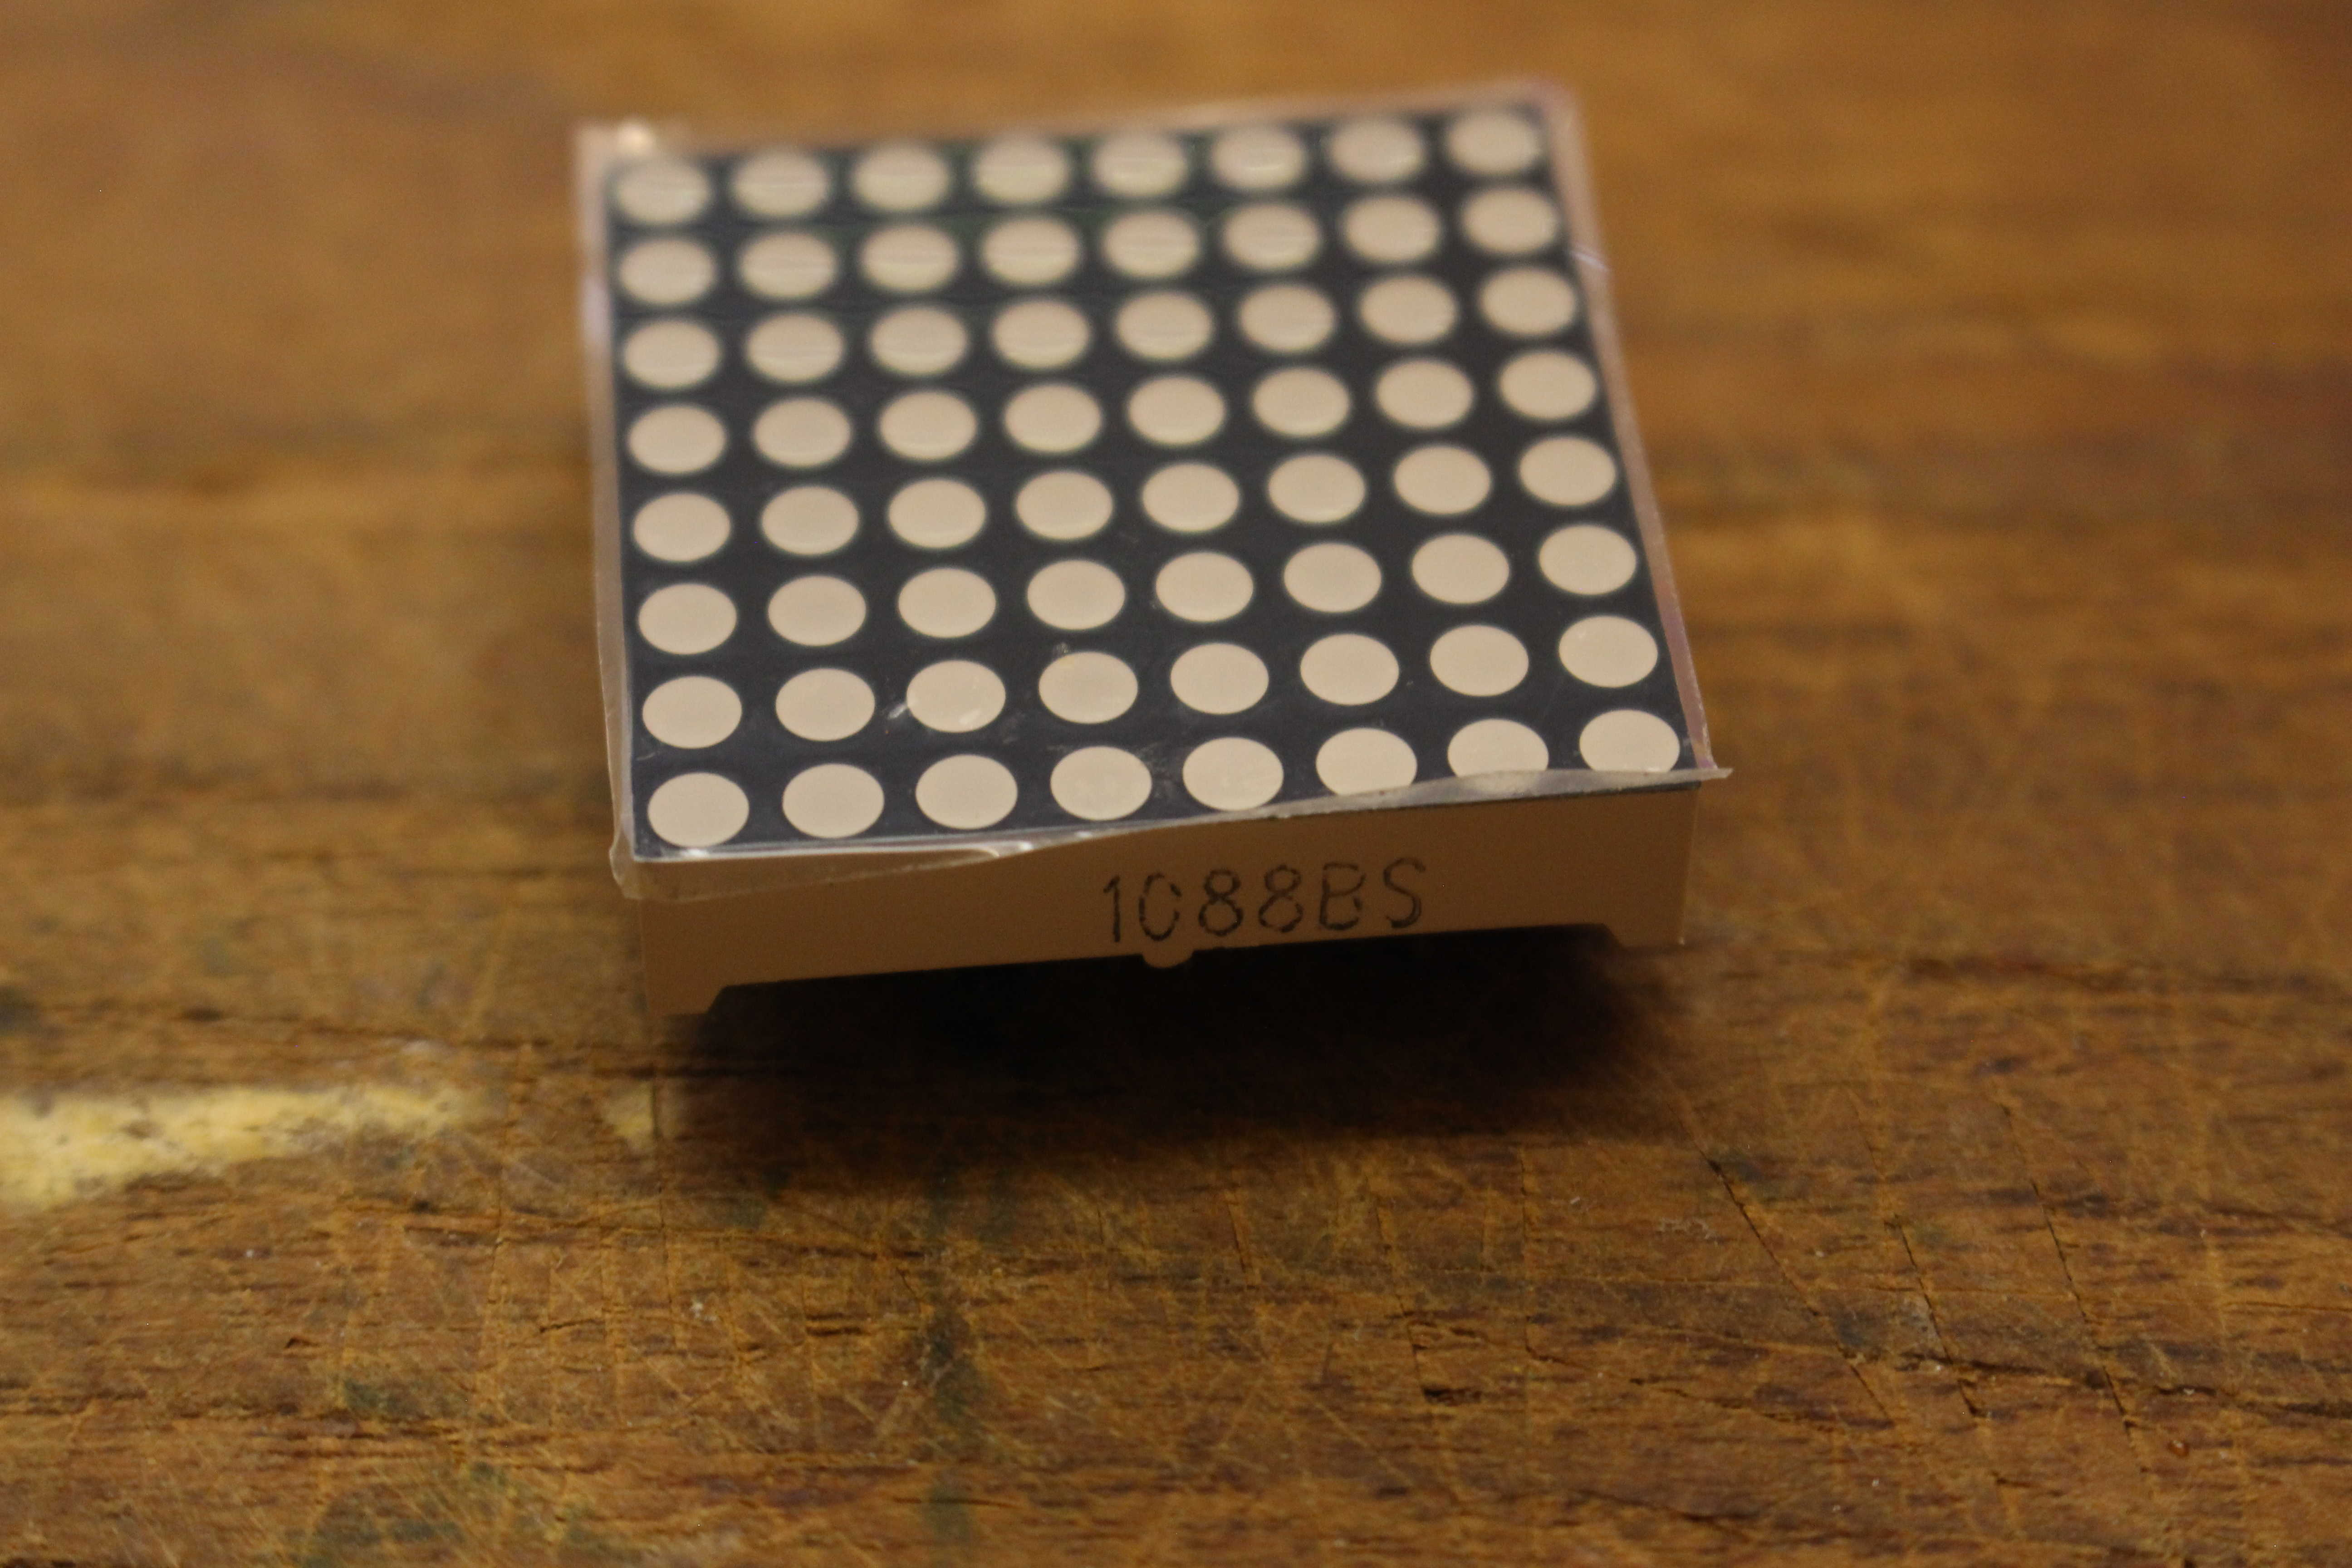
\includegraphics[width=\textwidth]{Bilder/IMG_5577.JPG}
	%\captionof{figure}{}
	%\label{fig:}
\end{minipage}
\begin{minipage}[b]{0.5\textwidth}
	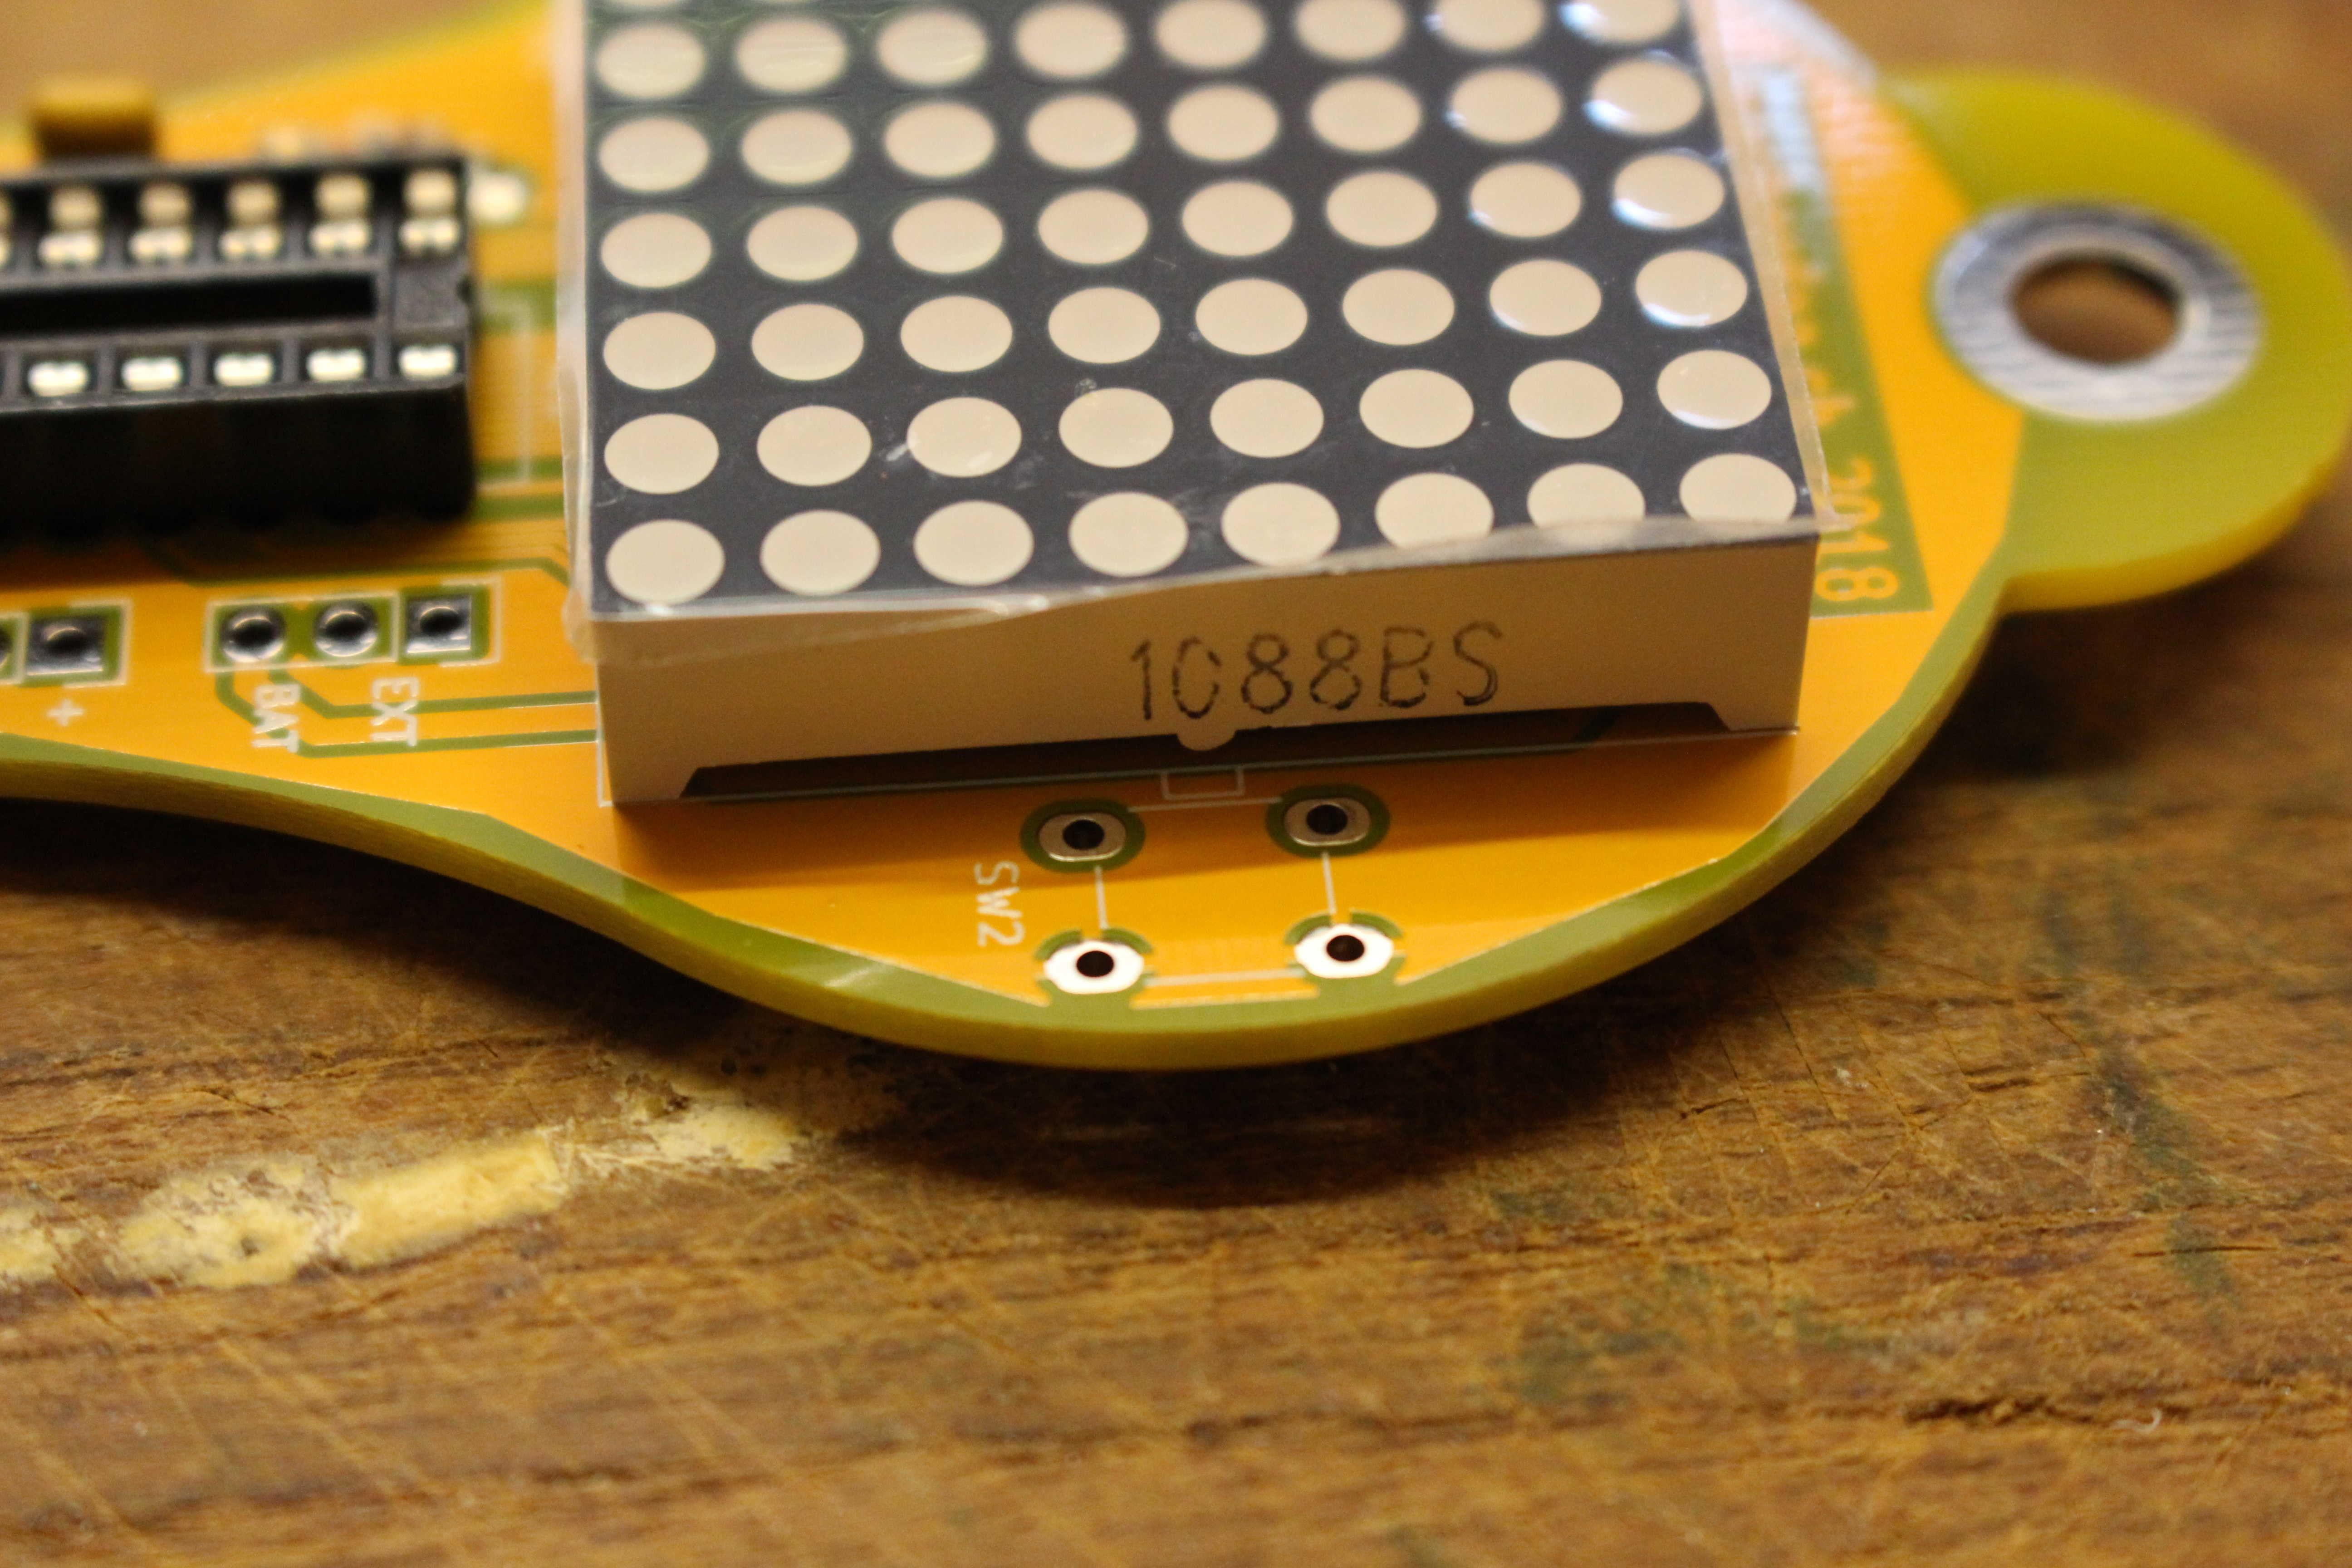
\includegraphics[width=\textwidth]{Bilder/IMG_5578.JPG}
	%\captionof{figure}{}
	%\label{fig:}
\end{minipage}

\vspace{0.5cm}

\begin{minipage}[b]{0.5\textwidth}
	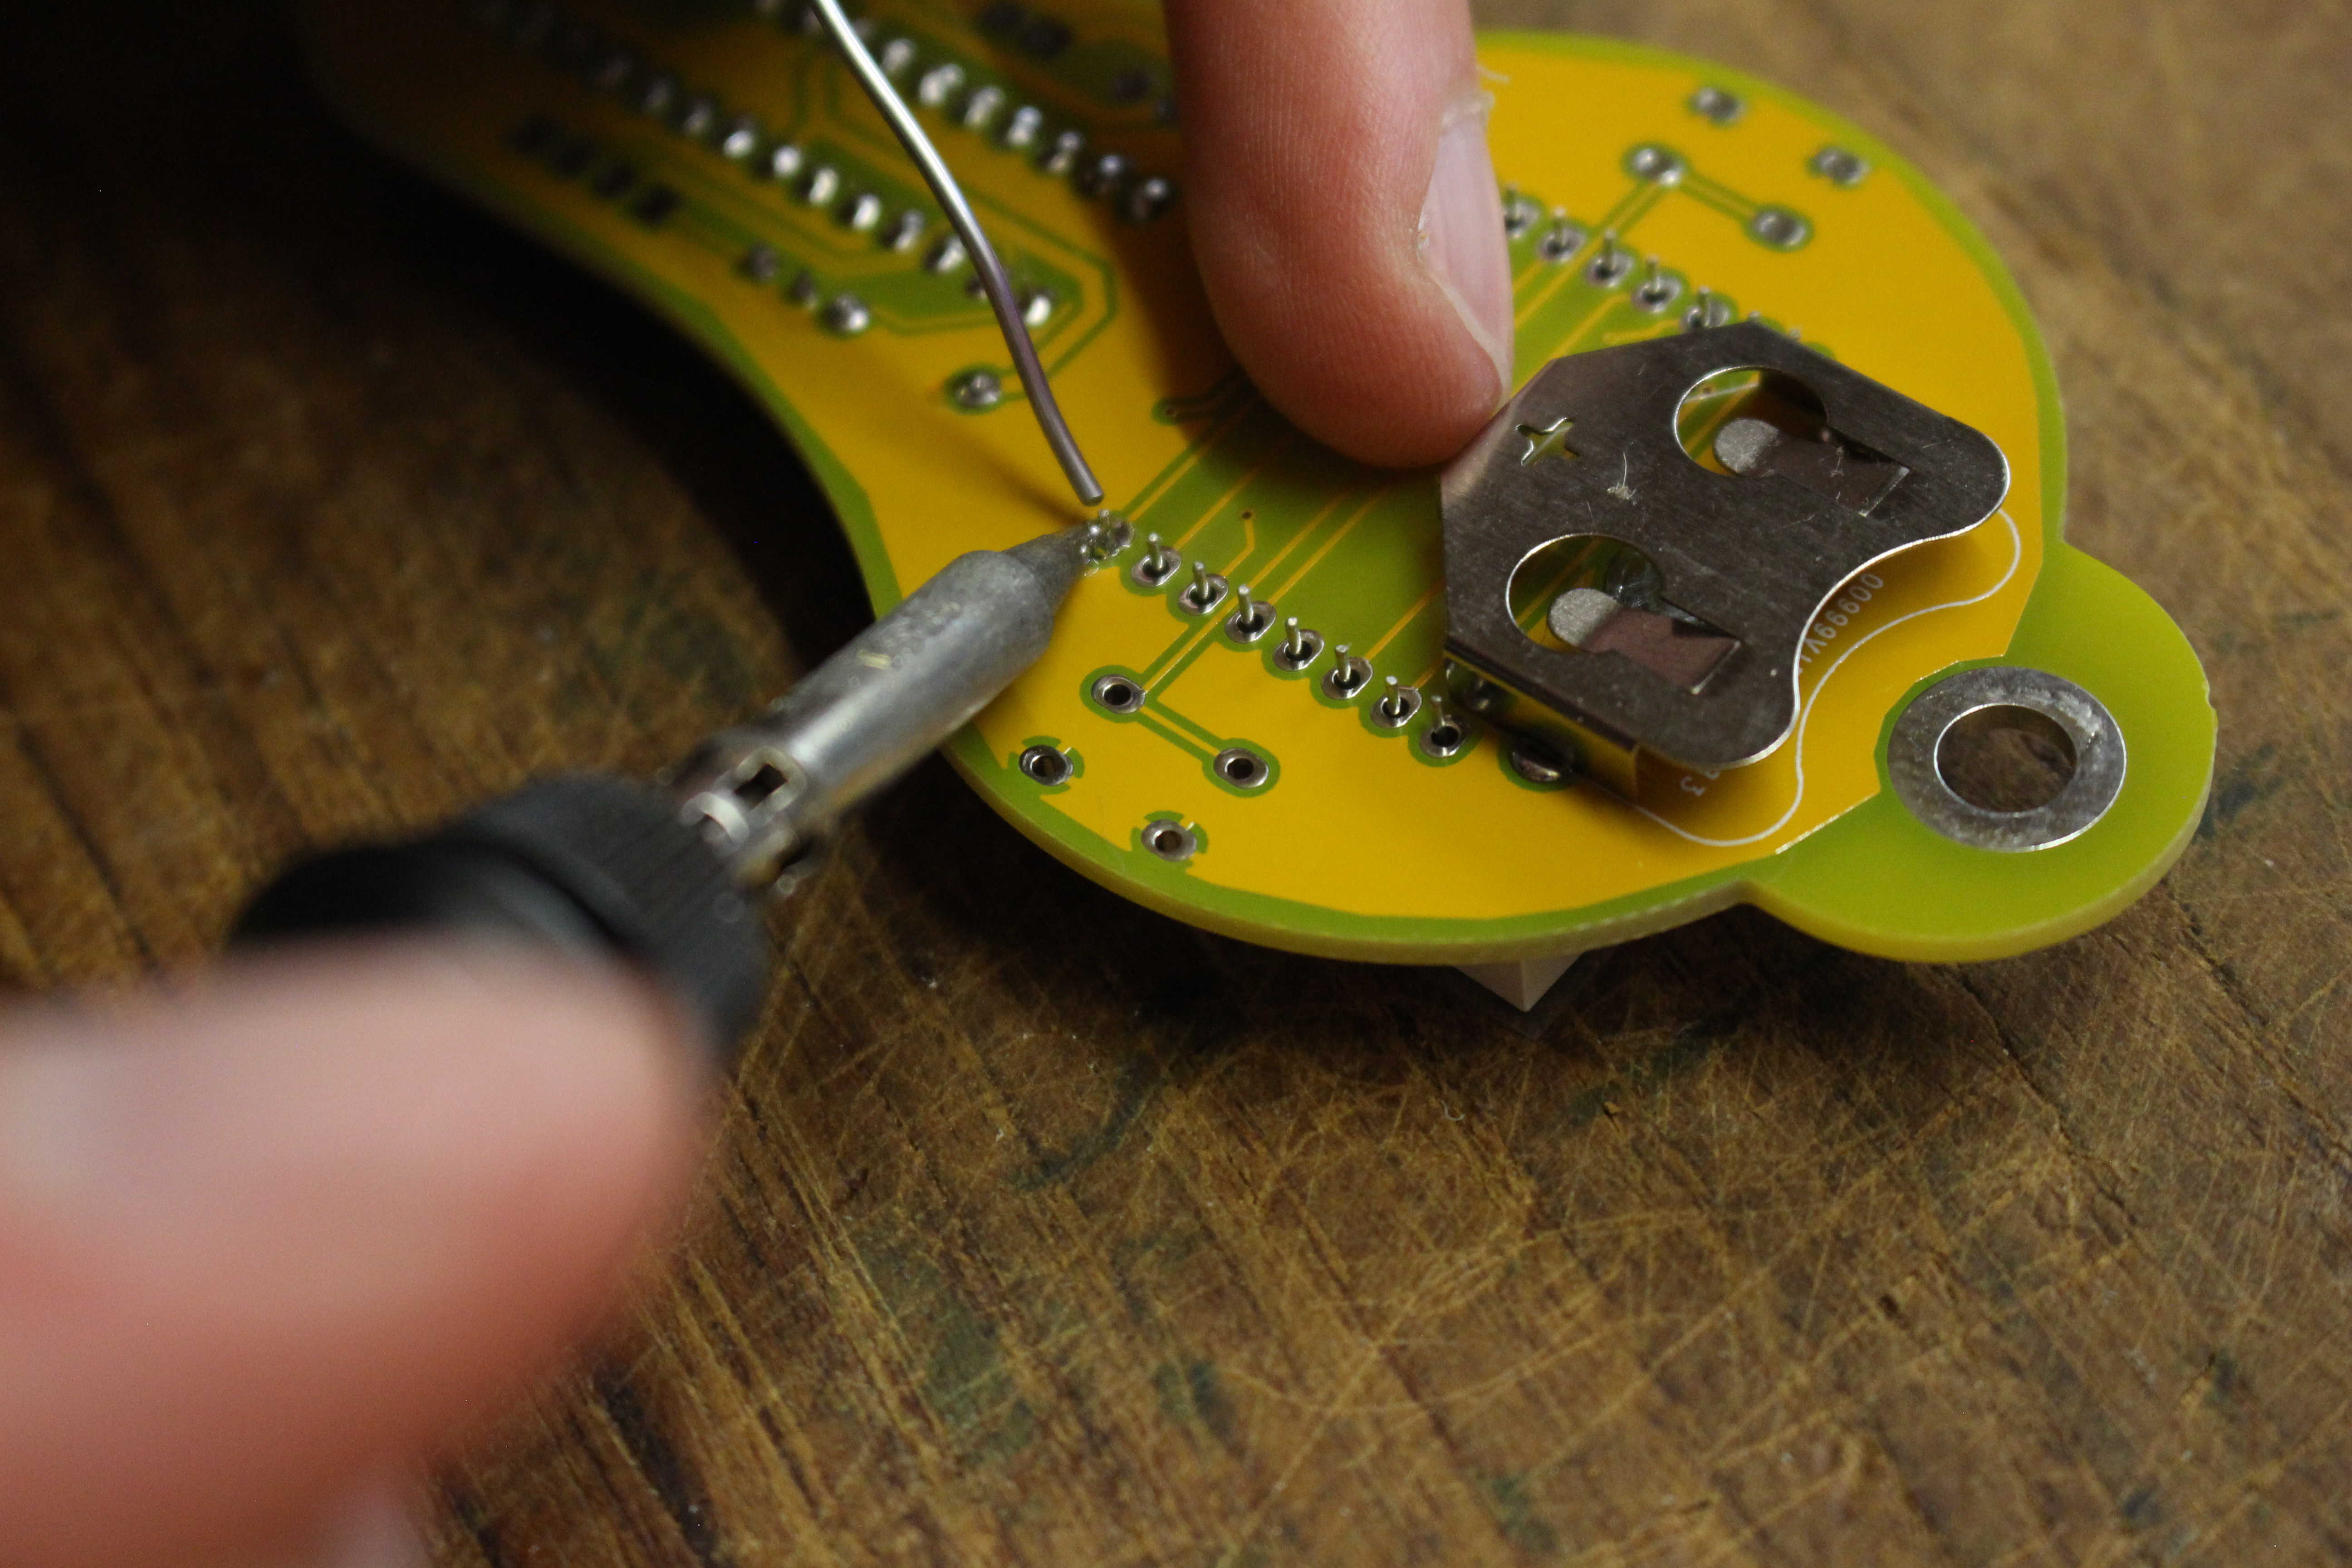
\includegraphics[width=\textwidth]{Bilder/IMG_5579.JPG}
	%\captionof{figure}{}
	%\label{fig:}
\end{minipage}
\begin{minipage}[b]{0.5\textwidth}
	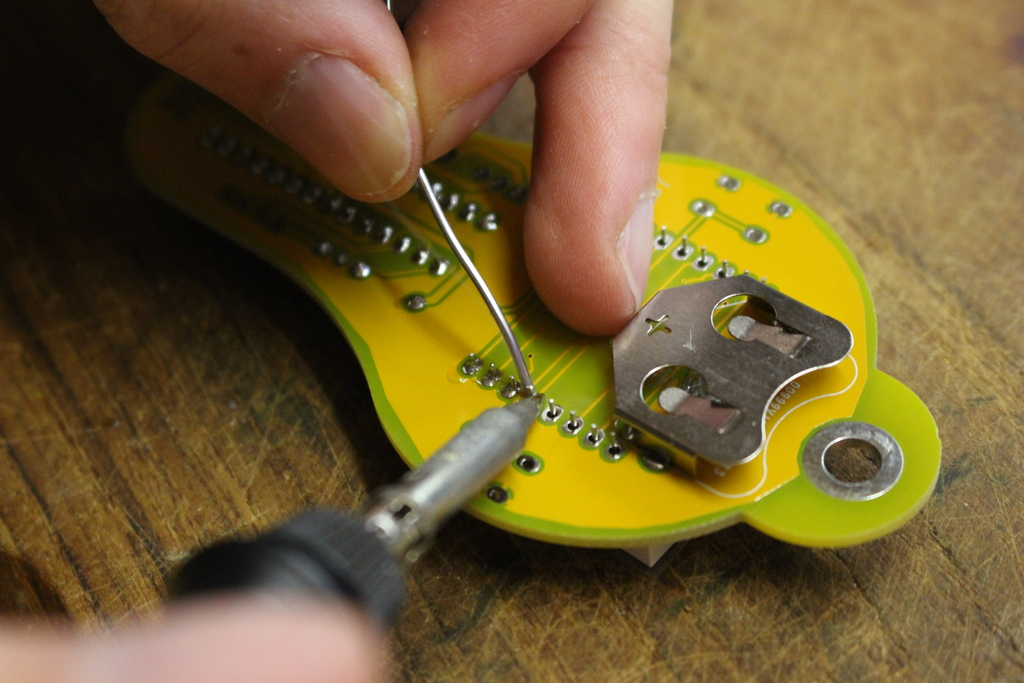
\includegraphics[width=\textwidth]{Bilder/IMG_5580.JPG}
	%\captionof{figure}{}
	%\label{fig:}
\end{minipage}

\subsection{Taster - SW1 und SW2}

Um die Taster in die Bohrlöcher zu bekommen, musst du ein bisschen fummeln. Wenn sie mal sitzen, fallen sie von alleine nicht mehr heraus und das Festlöten geht ganz einfach von der Hand.

Die Taster kann man zum Glück auch nicht falsch herum anlöten.

\vspace{1cm}

\begin{minipage}[b]{0.5\textwidth}
	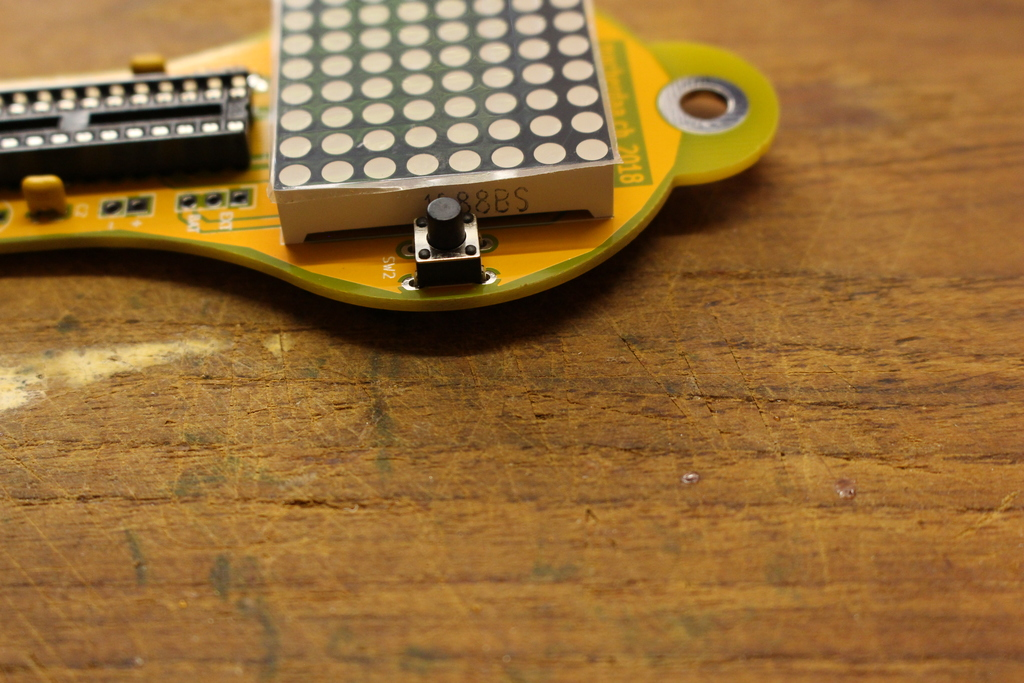
\includegraphics[width=\textwidth]{Bilder/IMG_5587.JPG}
	%\captionof{figure}{}
	%\label{fig:}
\end{minipage}
\begin{minipage}[b]{0.5\textwidth}
	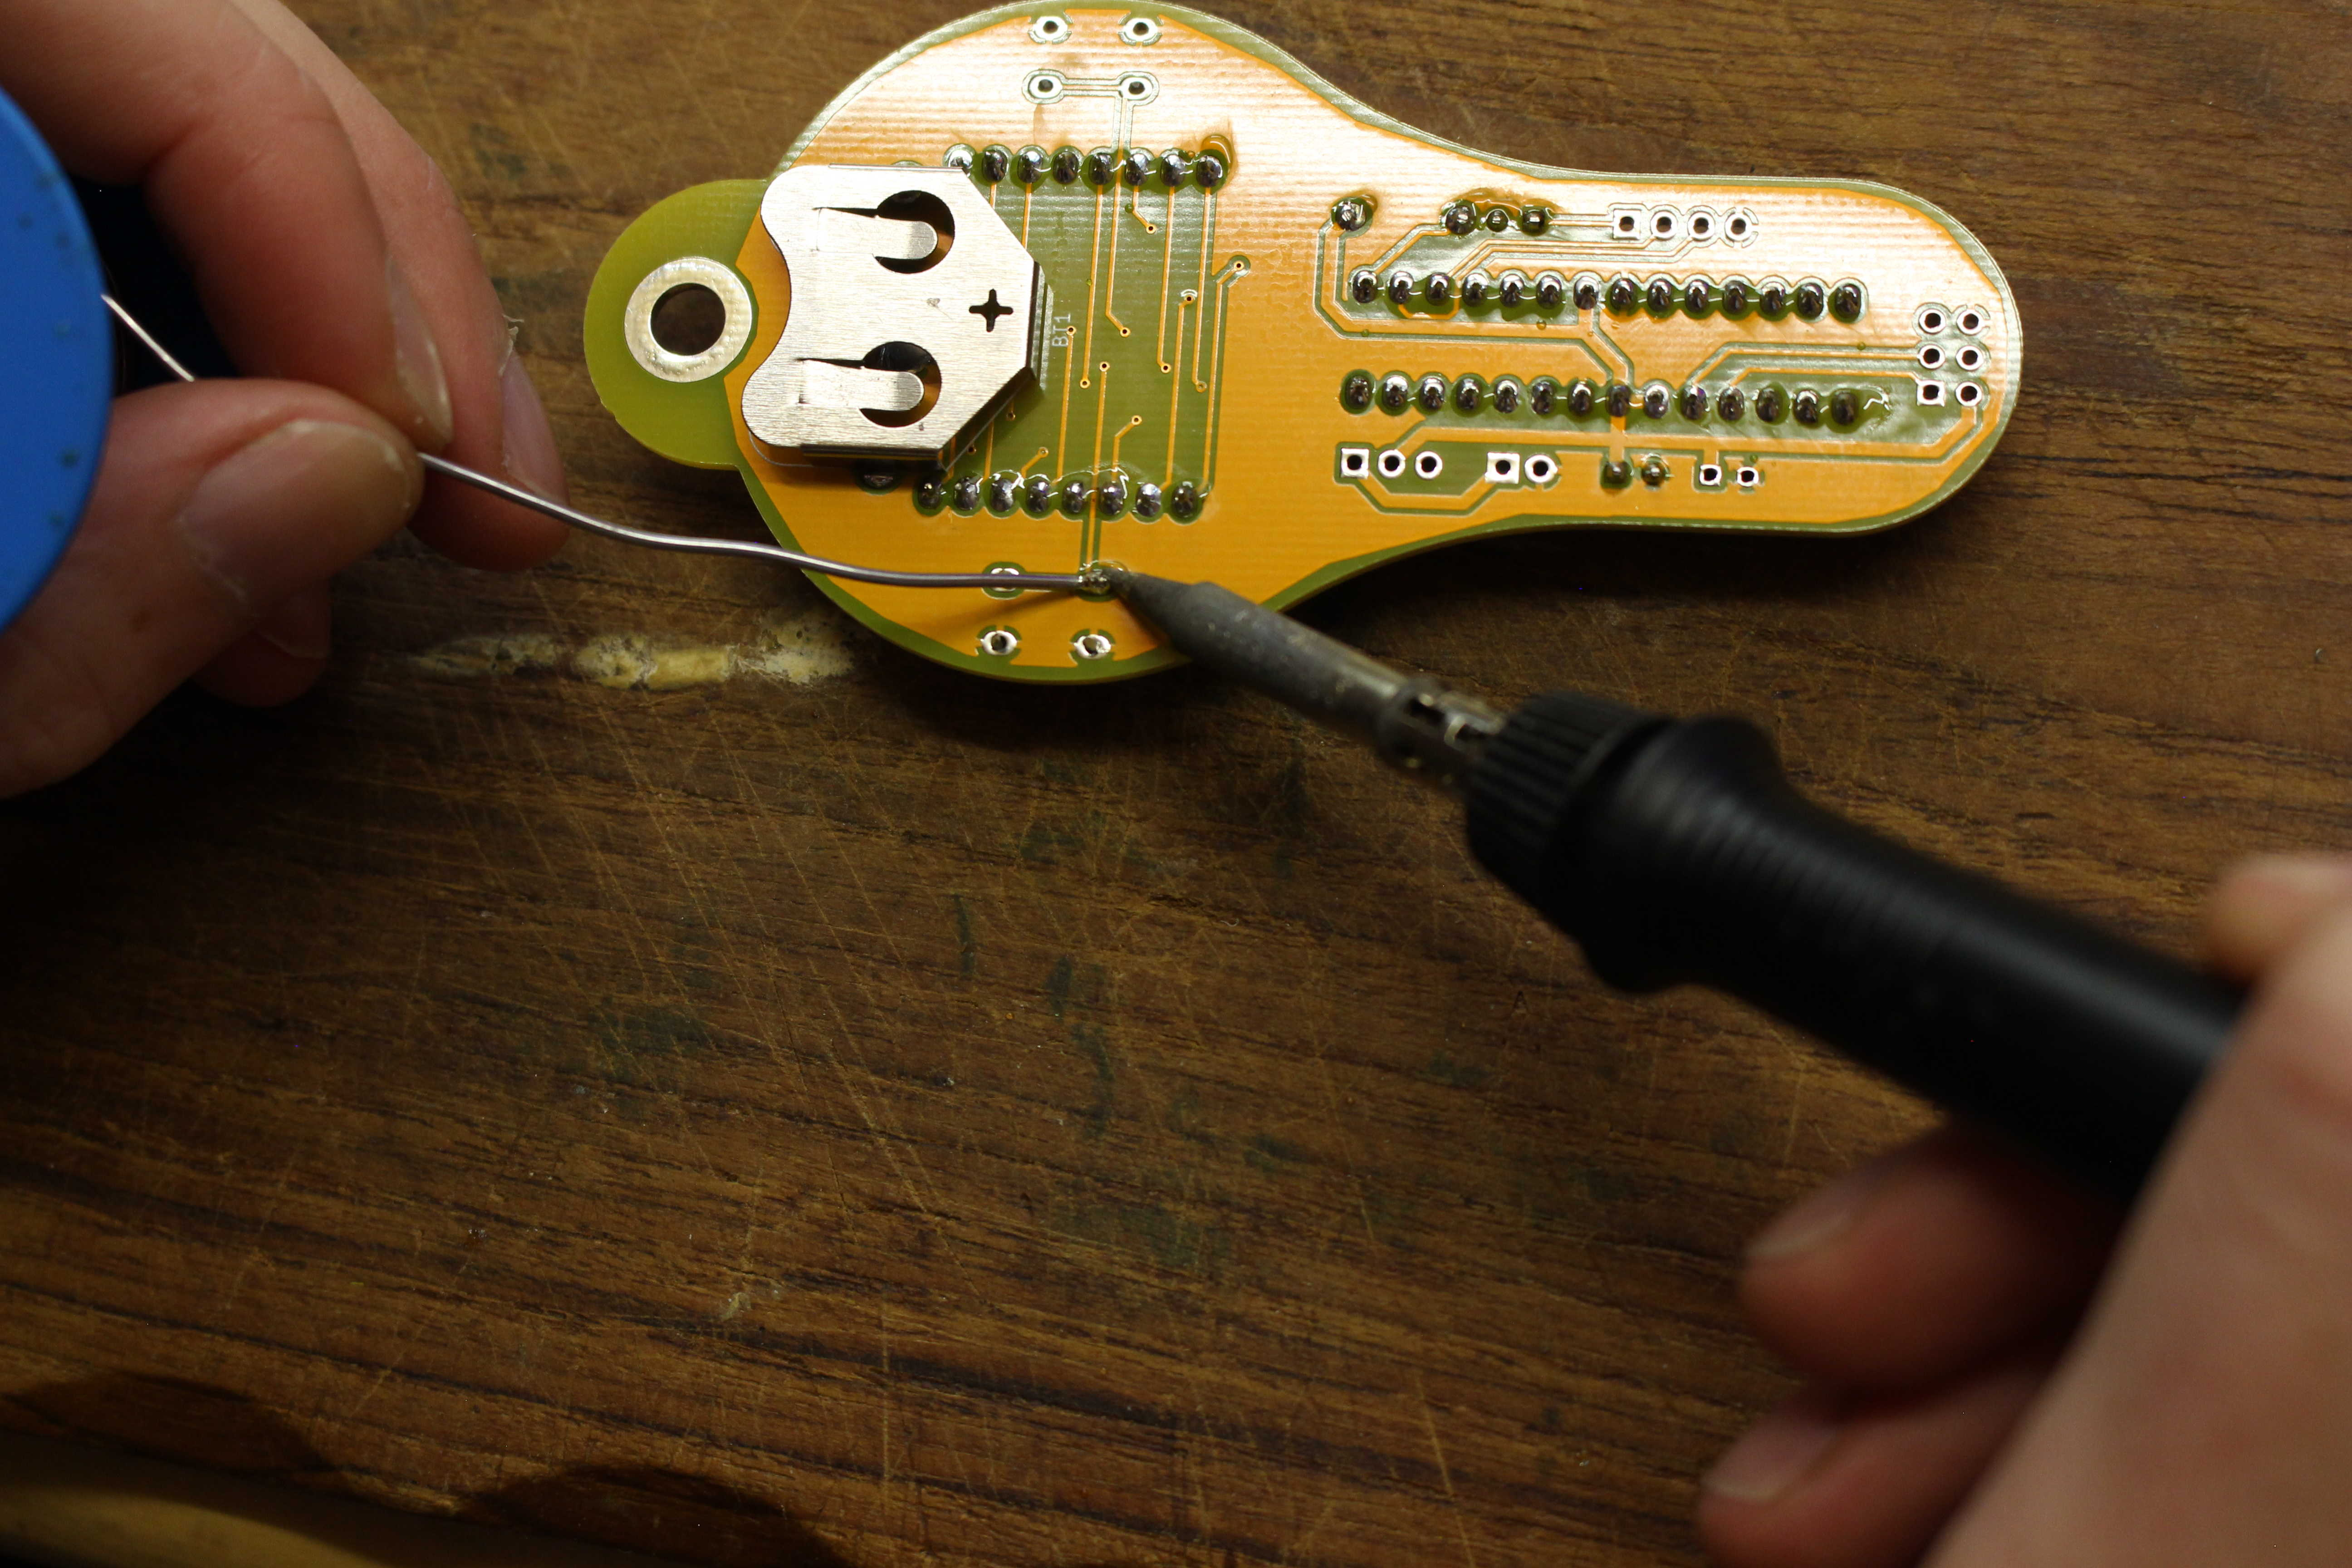
\includegraphics[width=\textwidth]{Bilder/IMG_5588.JPG}
	%\captionof{figure}{}
	%\label{fig:}
\end{minipage}

\vspace{0.5cm}

\begin{minipage}[b]{0.5\textwidth}
	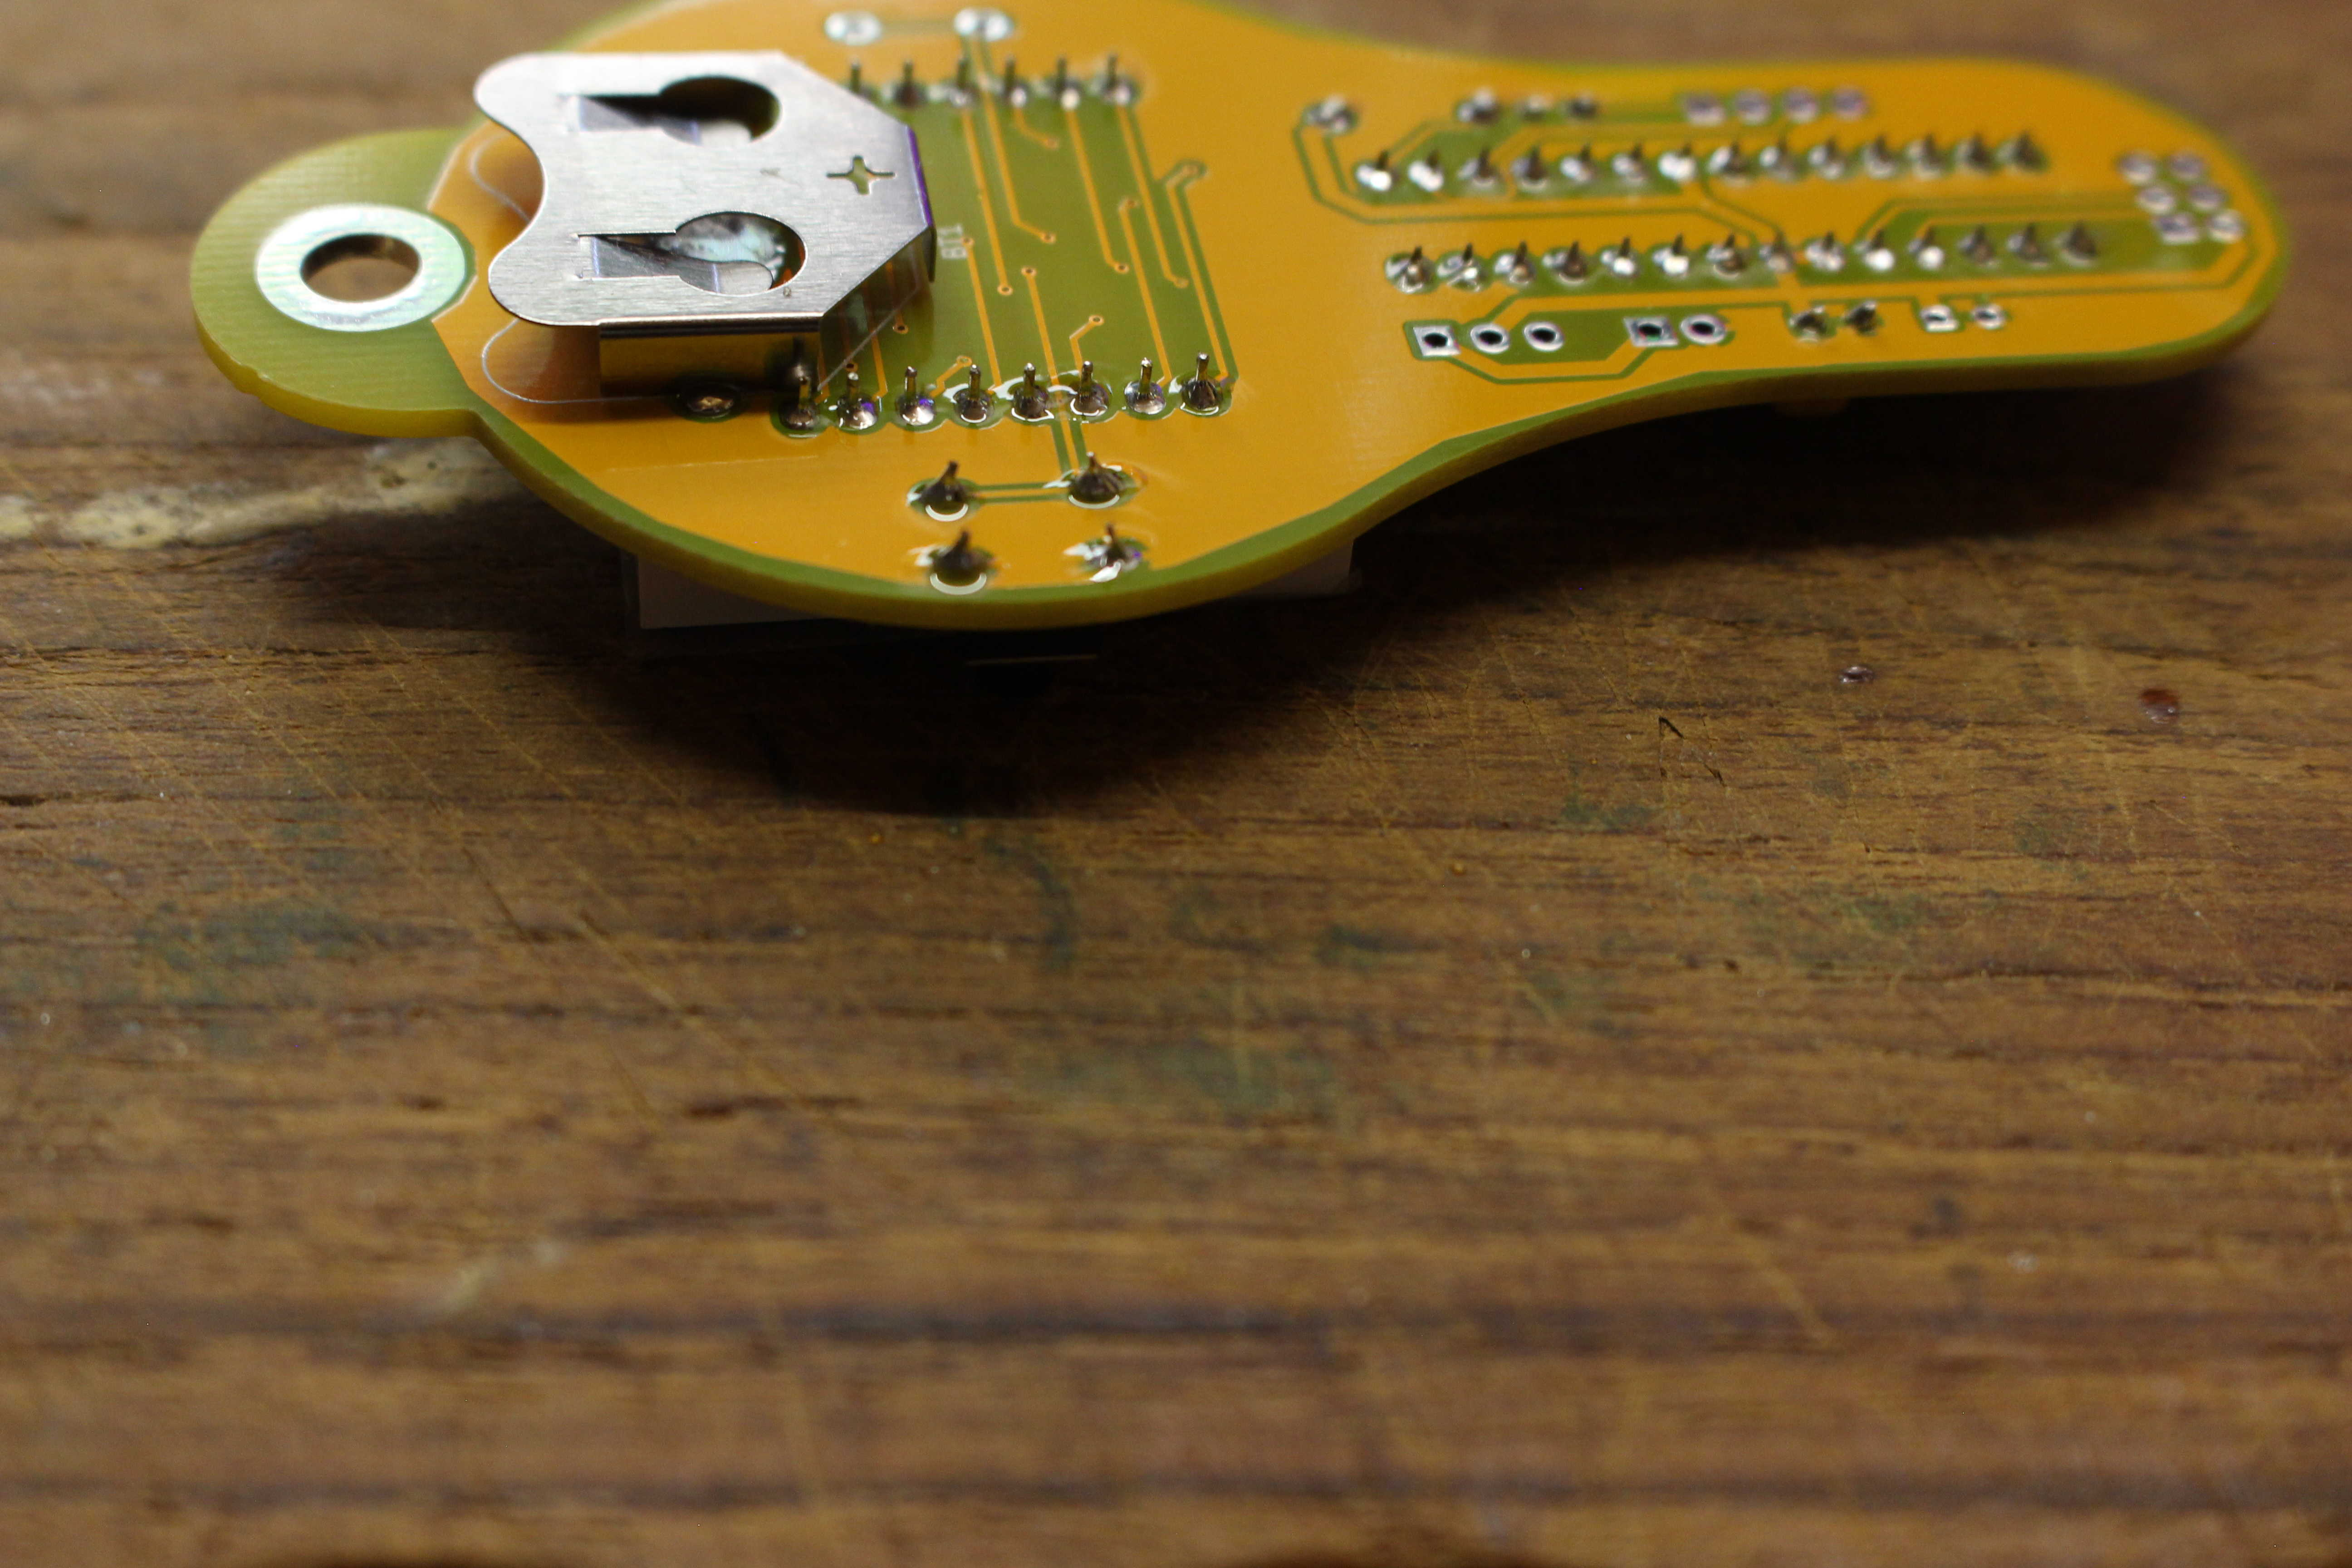
\includegraphics[width=\textwidth]{Bilder/IMG_5590.JPG}
	%\captionof{figure}{}
	%\label{fig:}
\end{minipage}
\begin{minipage}[b]{0.5\textwidth}
	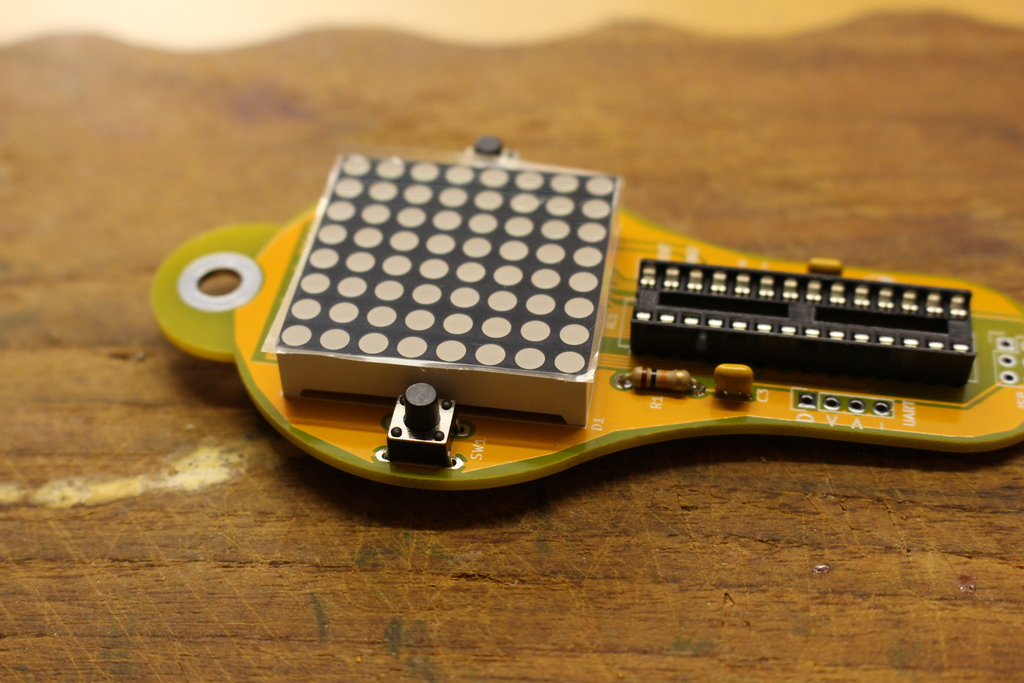
\includegraphics[width=\textwidth]{Bilder/IMG_5592.JPG}
	%\captionof{figure}{}
	%\label{fig:}
\end{minipage}

\subsection{Elektrolytkondensator - C1 (100$\mu$F)}

Beim Elektrolytkondensator, dem so genannten Elko, musst du wieder auf die richtige Polung achten. Der Minus-Pol ist am Elko mit einem schwarzen Strich markiert, wo ein kleines blaues Minus-Zeichen aufgedruckt ist.

Auf der Platine ist der Minus-Pol mit einem weiß ausgefüllten Halbkreis markiert.

\vspace{1cm}

\begin{minipage}[b]{0.5\textwidth}
	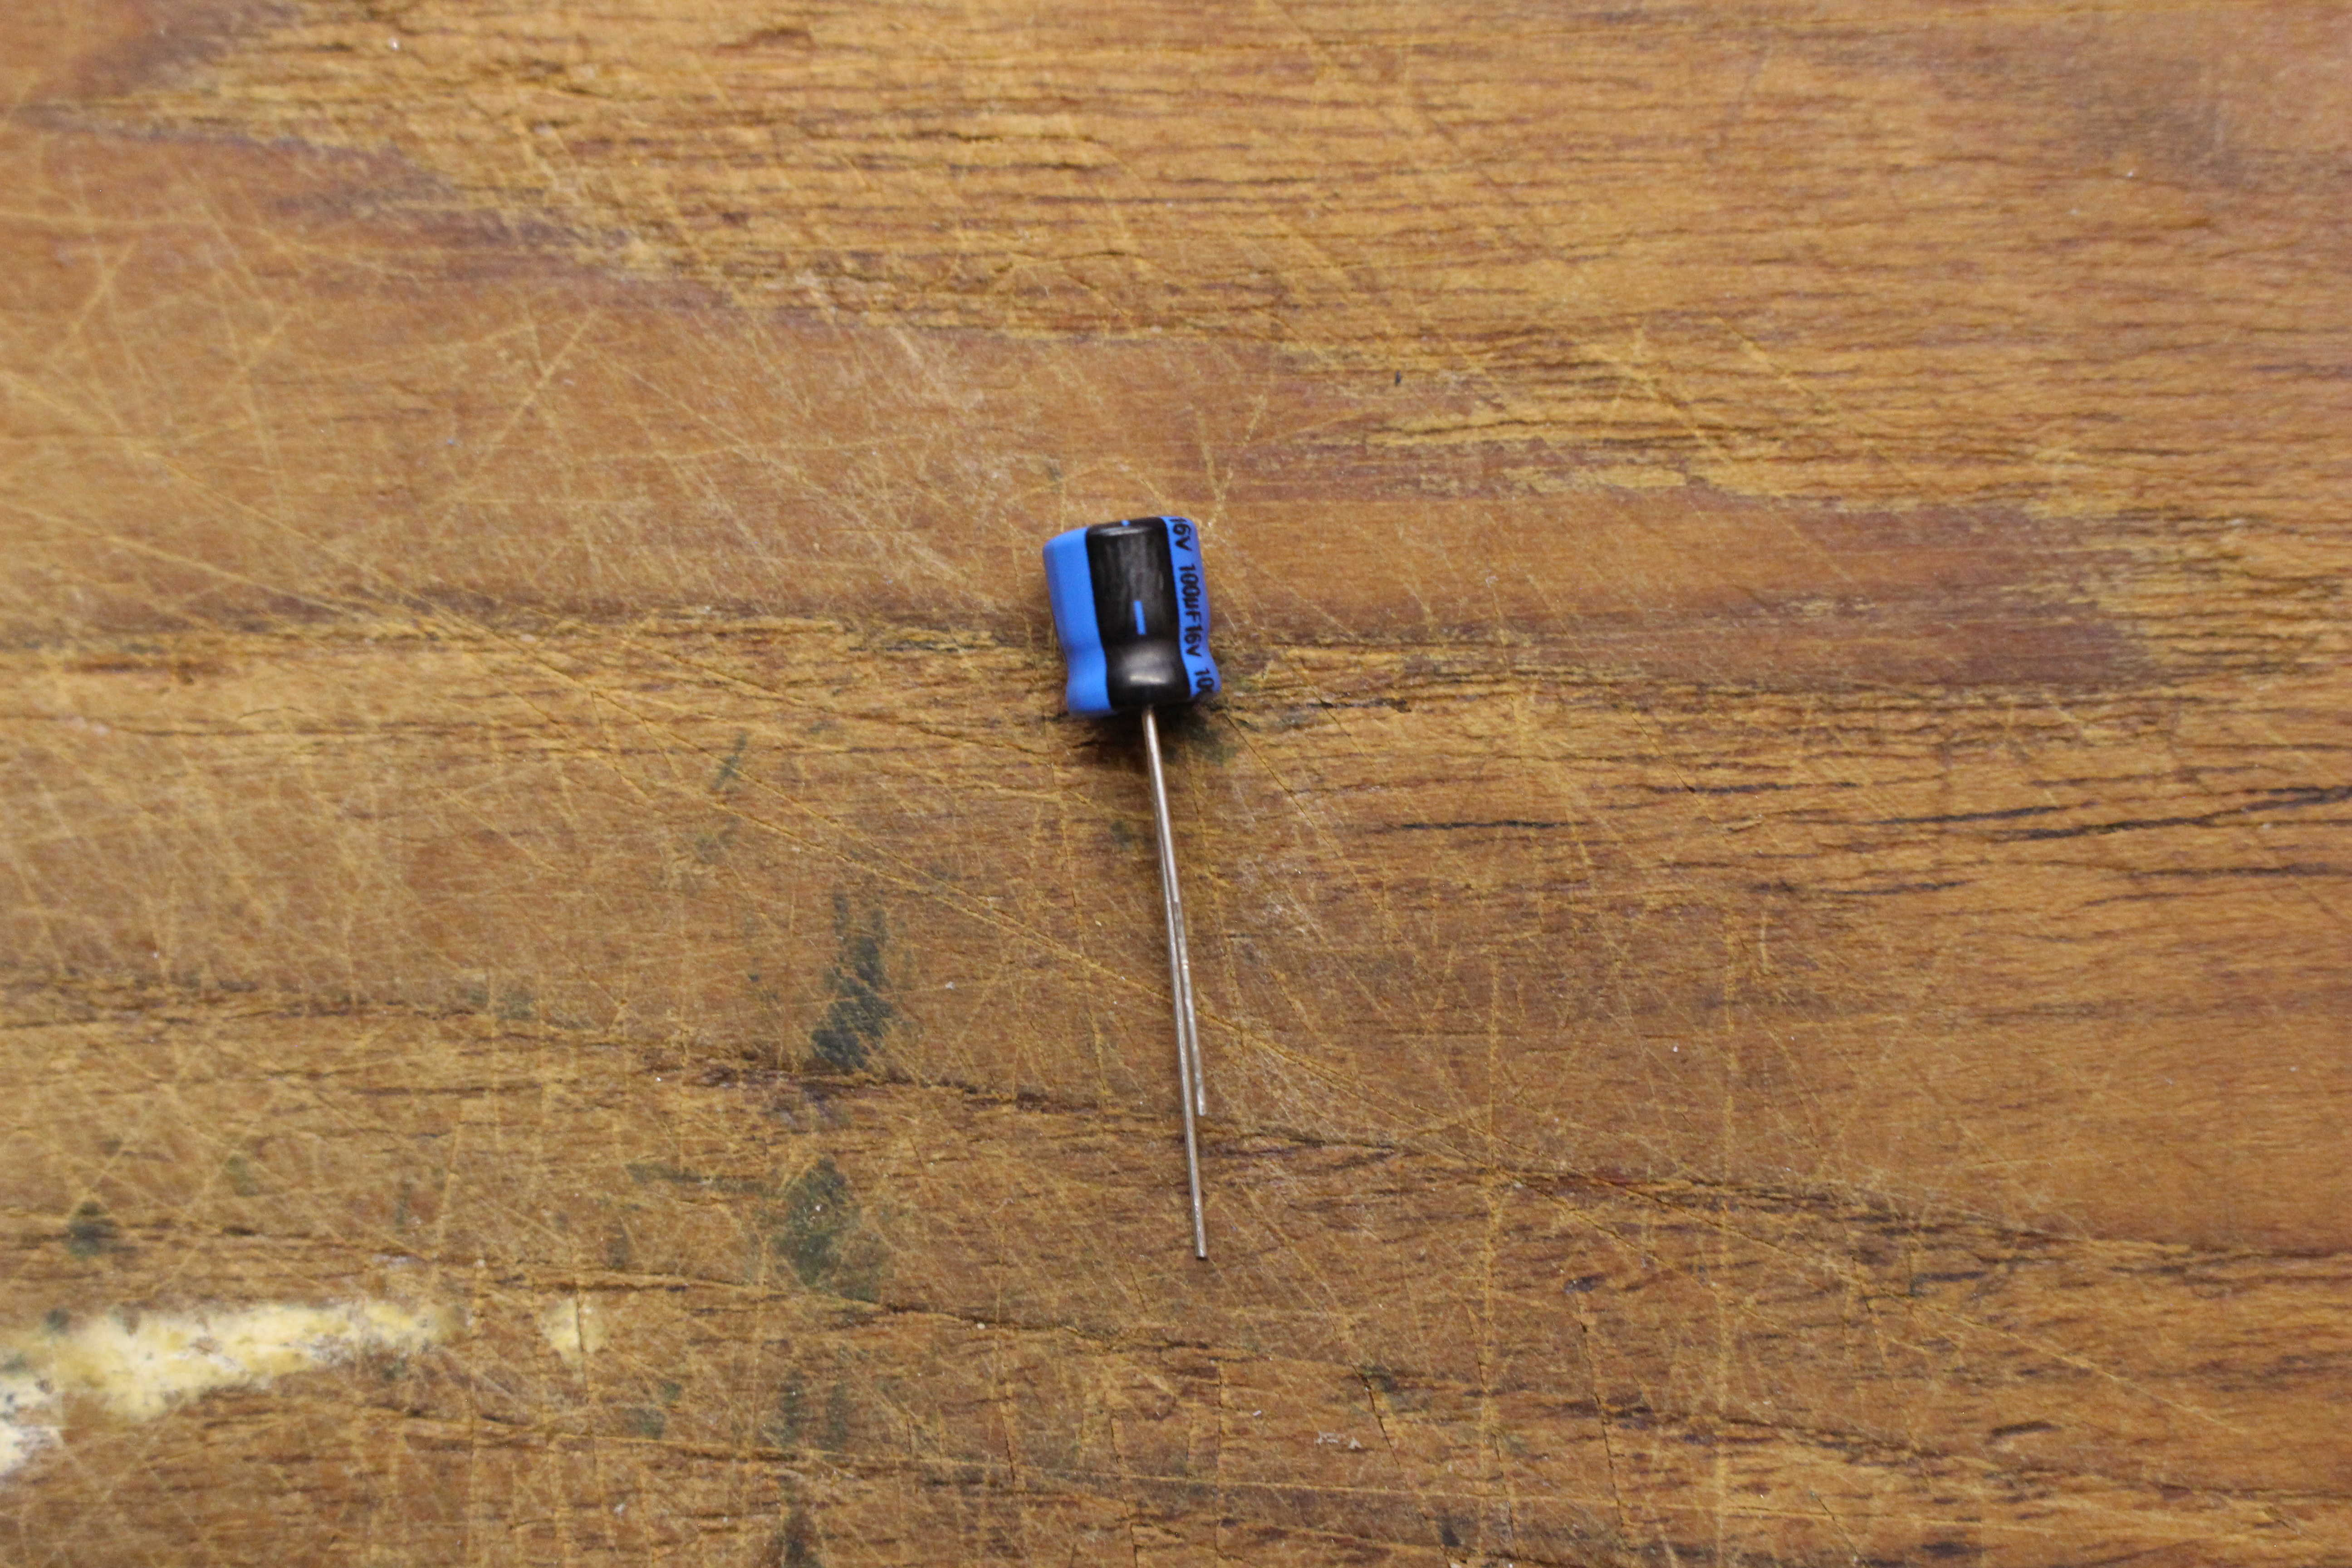
\includegraphics[width=\textwidth]{Bilder/IMG_5593.JPG}
	%\captionof{figure}{}
	%\label{fig:}
\end{minipage}
\begin{minipage}[b]{0.5\textwidth}
	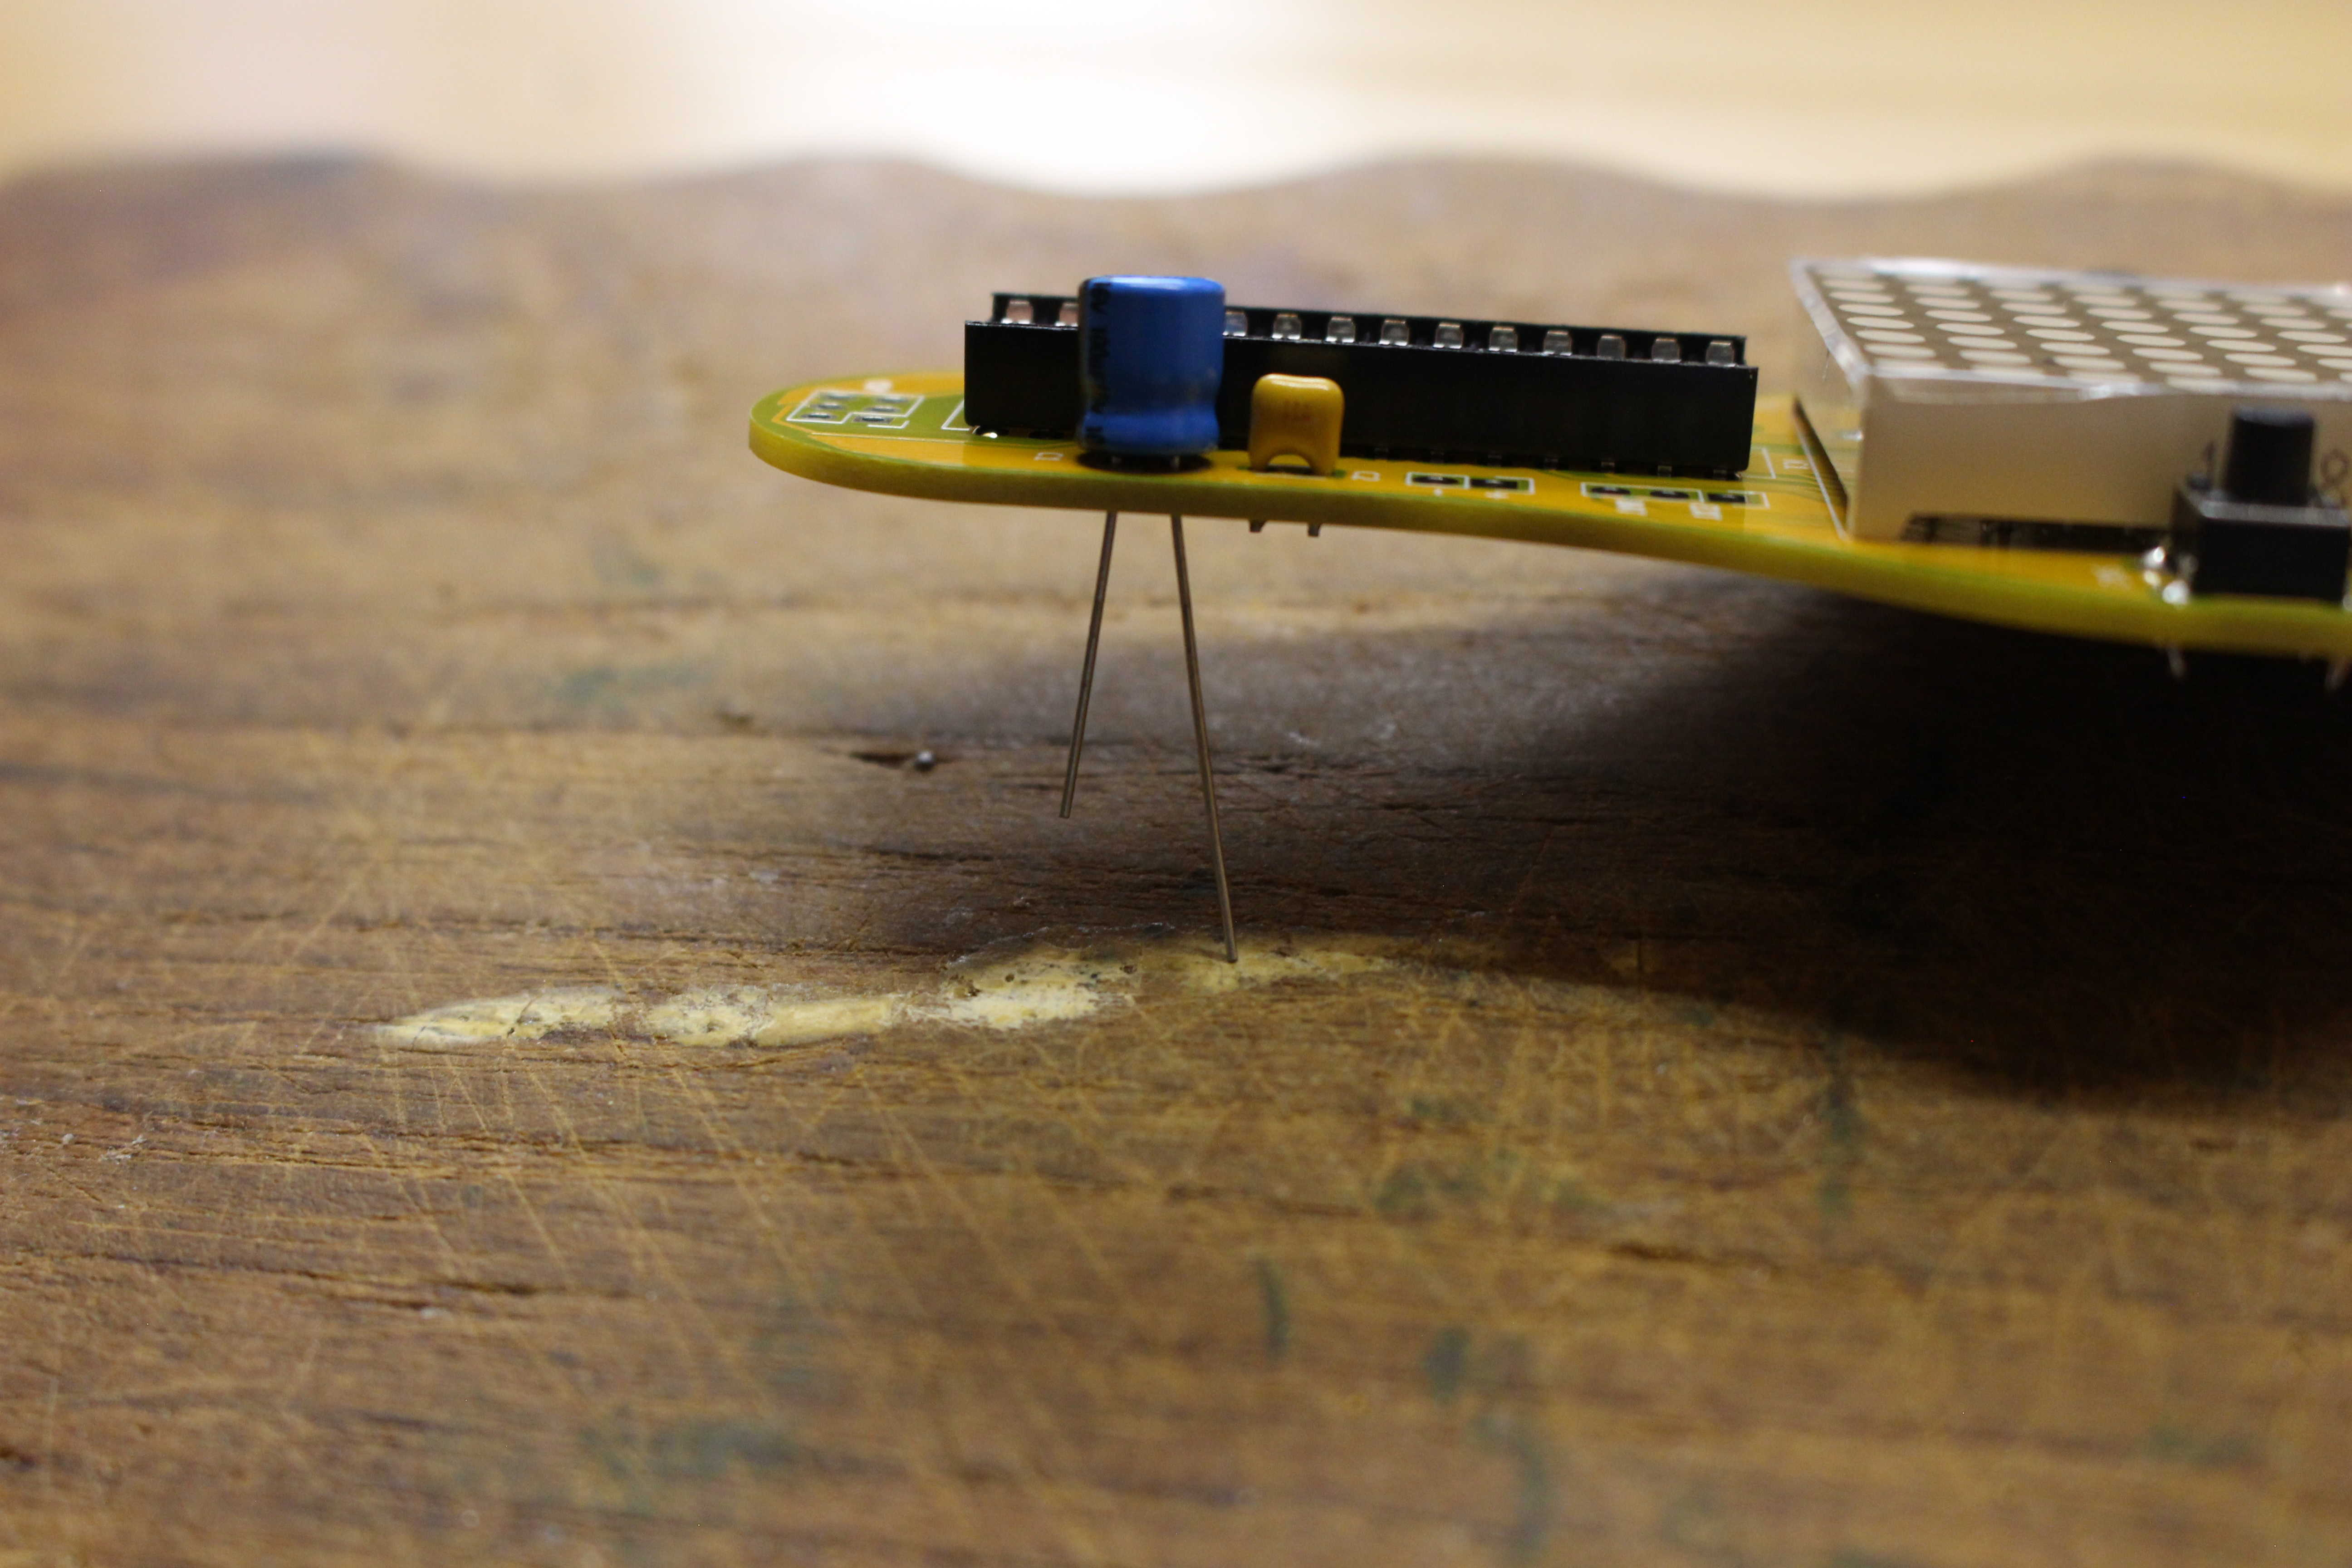
\includegraphics[width=\textwidth]{Bilder/IMG_5594.JPG}
	%\captionof{figure}{}
	%\label{fig:}
\end{minipage}

\vspace{0.5cm}

\begin{minipage}[b]{0.5\textwidth}
	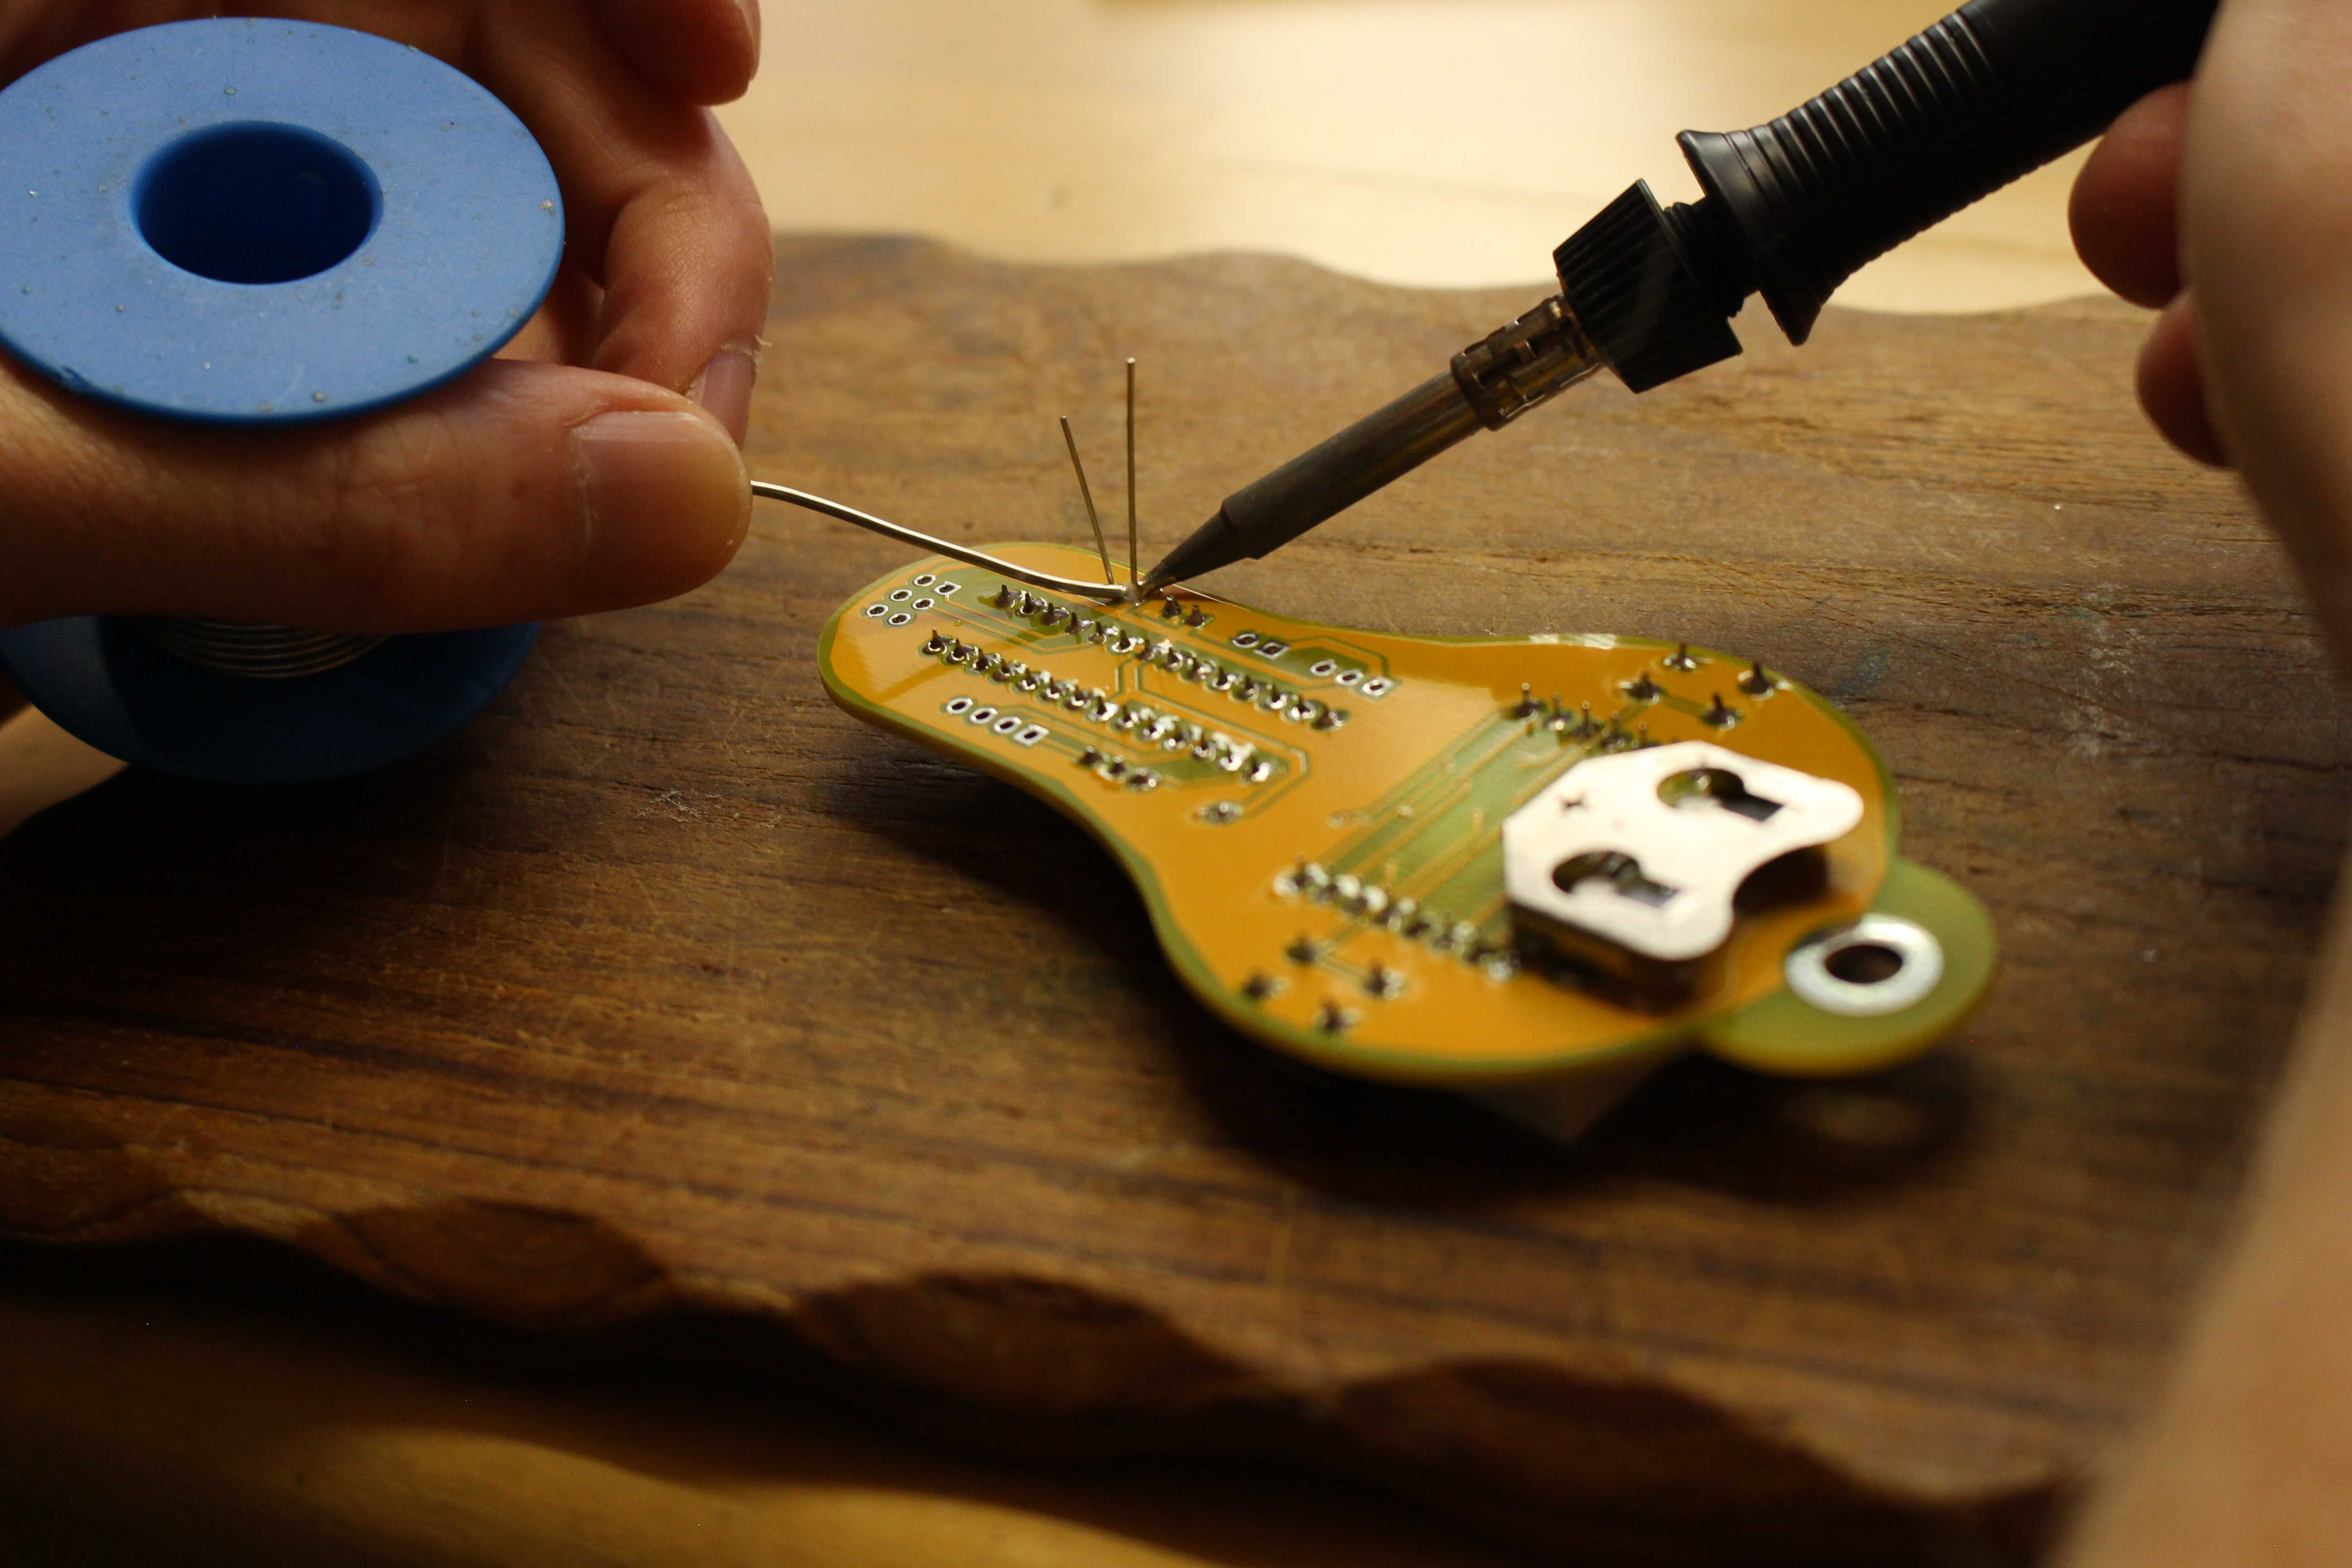
\includegraphics[width=\textwidth]{Bilder/IMG_5597.JPG}
	%\captionof{figure}{}
	%\label{fig:}
\end{minipage}
\begin{minipage}[b]{0.5\textwidth}
	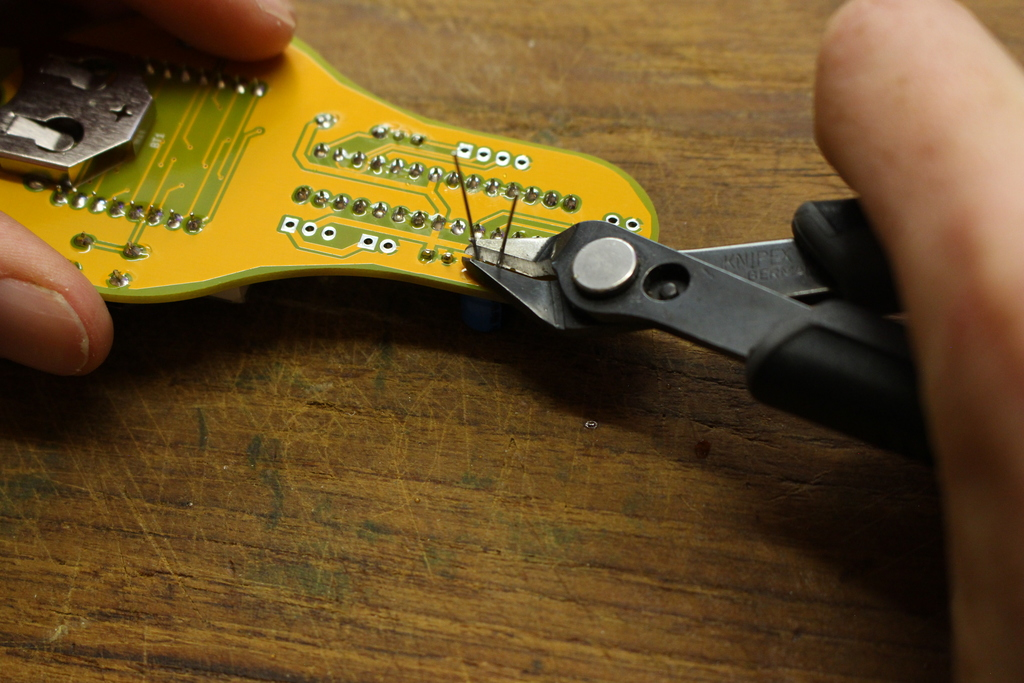
\includegraphics[width=\textwidth]{Bilder/IMG_5600.JPG}
	%\captionof{figure}{}
	%\label{fig:}
\end{minipage}

\subsection{Stiftleisten}

Wenn du Glück hast, dann wurden alle Stiftleisten schon vorbereitet.
Wenn du Pech hast, musst du sie selbst abzwicken.

Dazu nimmst du zuerst die einreihige Stiftleiste und die Zange und knipst erst 2, dann 3 und 4 Pins ab. Anschließend nimmst du die zweireihige Stiftleiste und zwickst 3 Pins (insgesamt 6) ab. Achtung! Die zweireihigen Stiftleisten lassen sich nicht immer so einfach abzwicken. Es kann sein, dass du mehrere Anläufe brauchst.

Das Anlöten der Stiftleisten ist der schwierigste Teil, den du bewältigen musst. Das Problem ist, dass wir zu wenige Hände haben und uns deshalb etwas einfallen lassen müssen. Damit wir keine Hand zum Halten des Lötzinns brauchen, legen wir die Rolle mit Lötzinn auf den Tisch und biegen uns das Lötzinn so zurecht, dass das Ende später auf die Platine zeigt.

Eine weitere Schwierigkeit ist, dass sich die einreihigen Stiftleisten nicht so gerne gerade auflöten lassen. Besonders wenn man mit dem Finger auf die Metallspitzen drückt um die Leiste an der Platine zu fixieren.

Deshalb drückst du am besten mit dem Fingernagel auf den Plastikteil der Stiftleiste. Das hat außerdem den Vorteil, dass du dir beim Festlöten nicht so leicht die Finger verbrennst.

\vspace{1cm}

\begin{minipage}[b]{0.5\textwidth}
	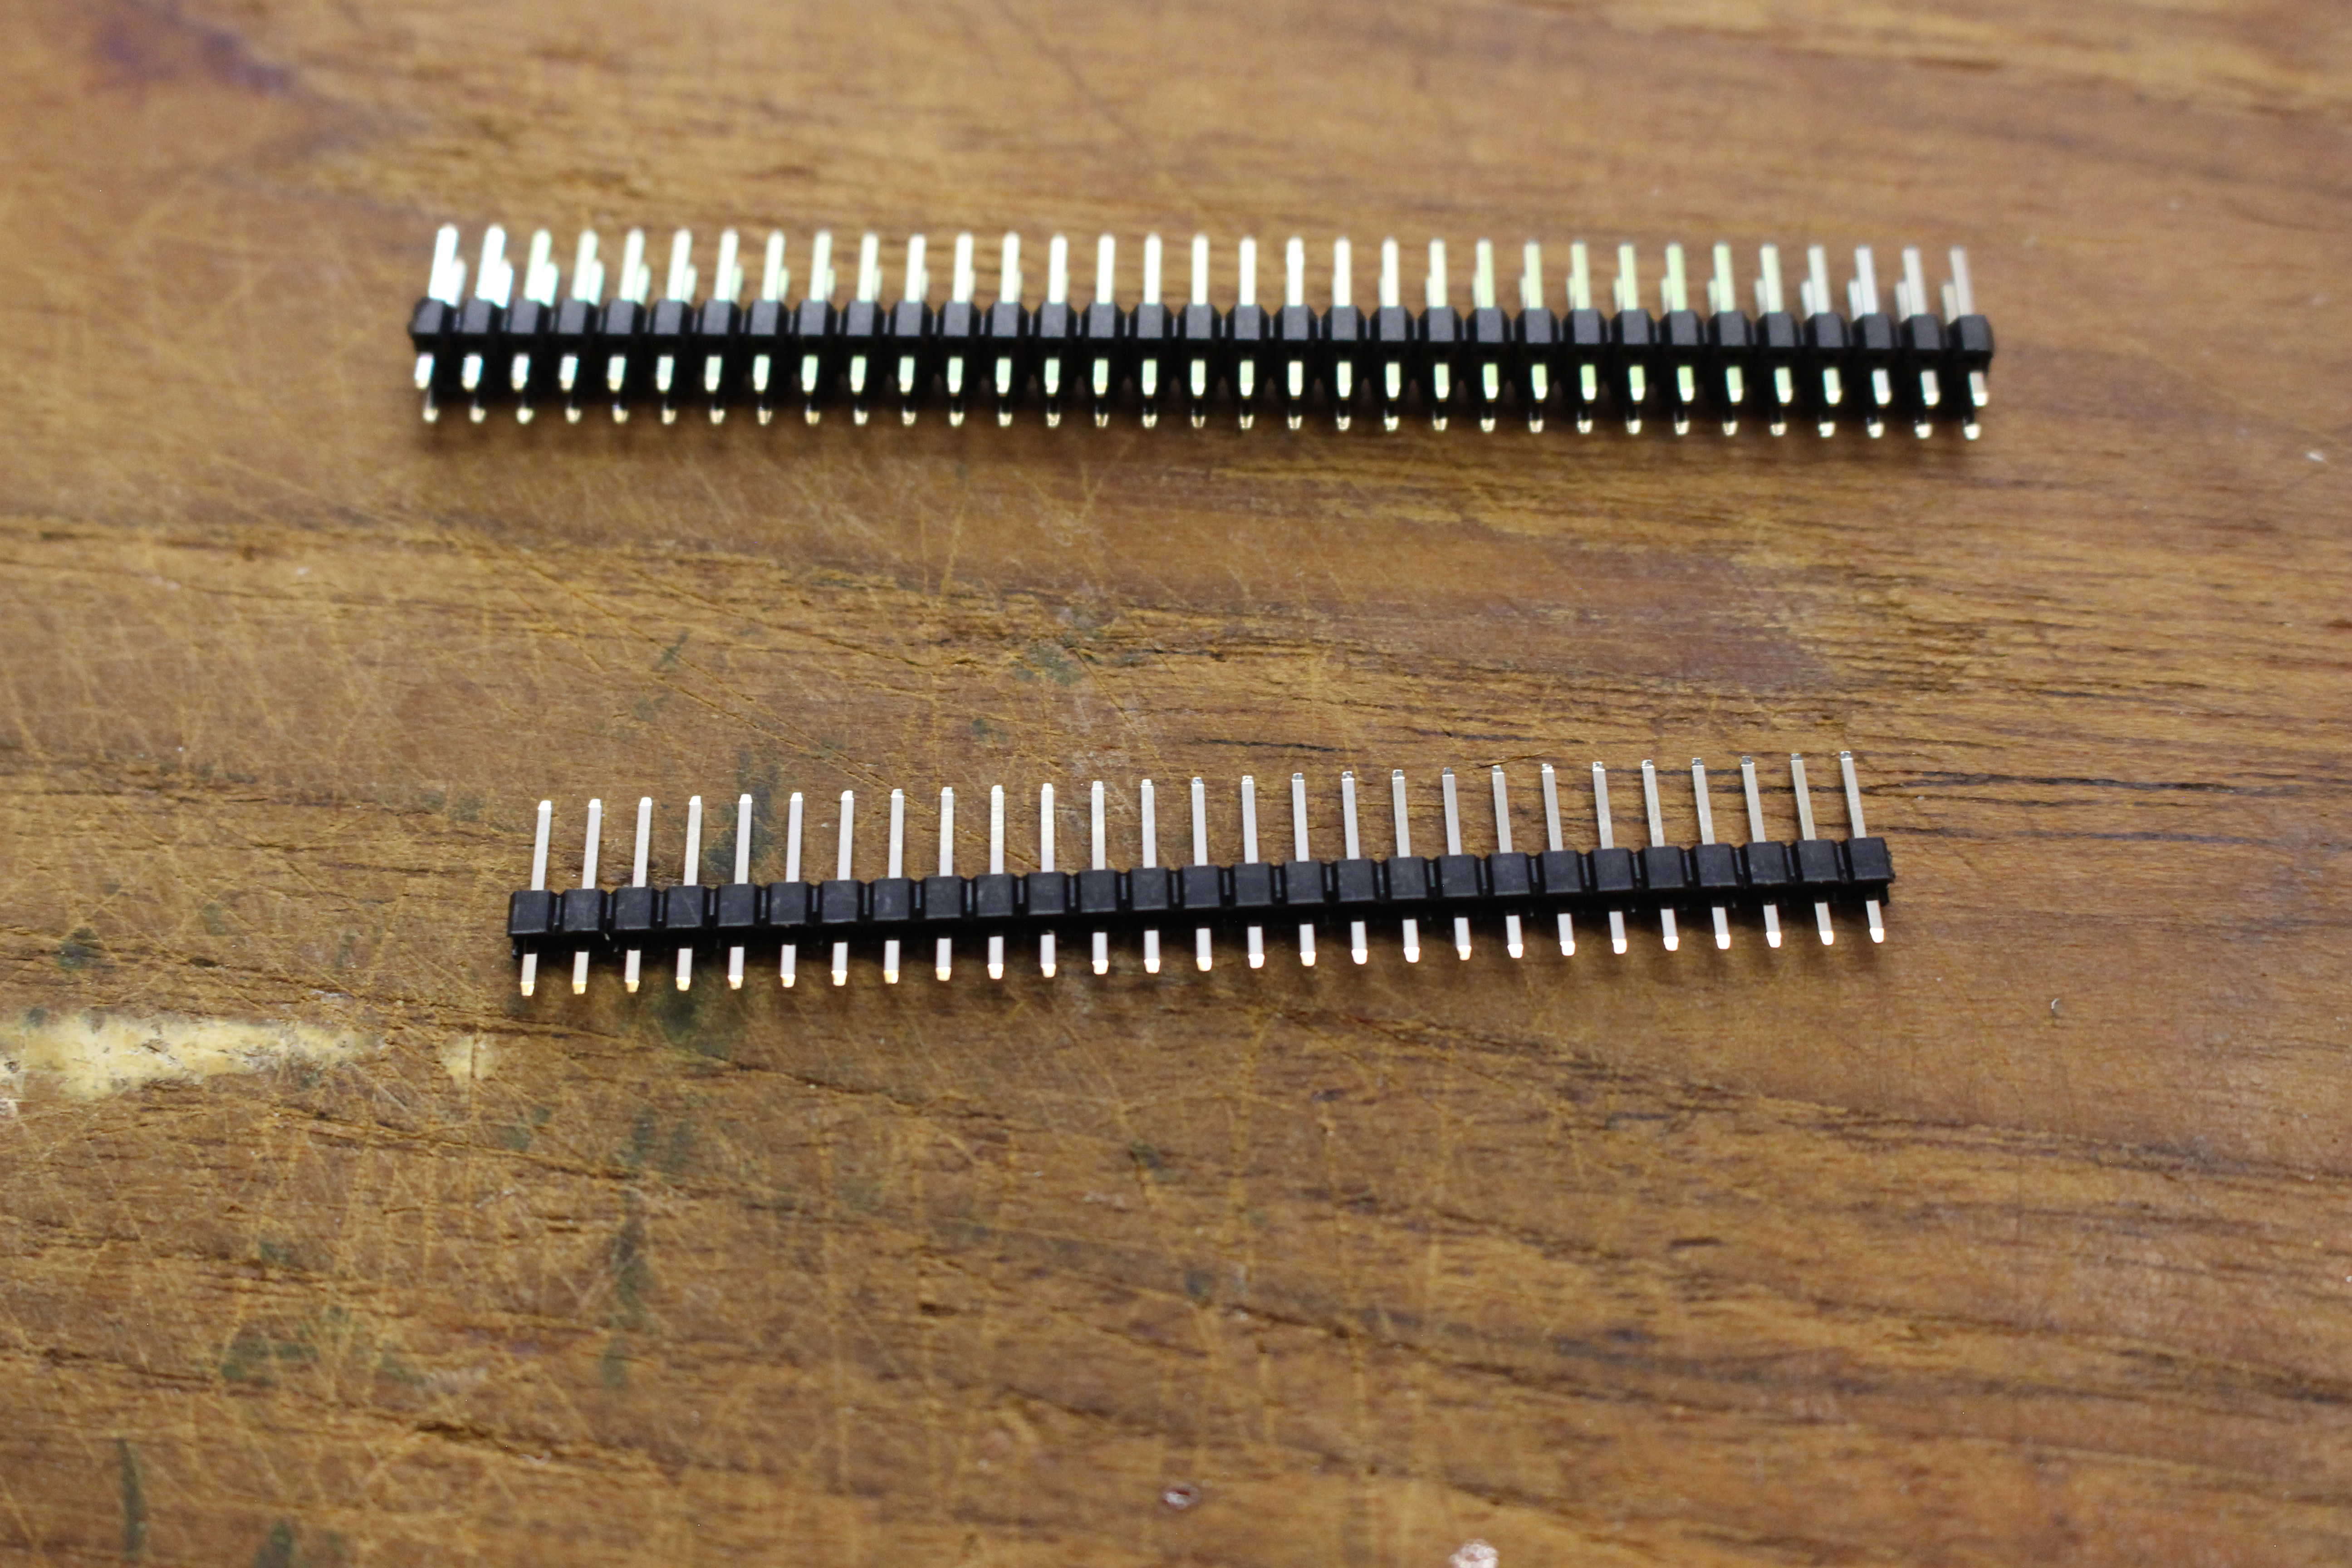
\includegraphics[width=\textwidth]{Bilder/IMG_5601.JPG}
	%\captionof{figure}{}
	%\label{fig:}
\end{minipage}
\begin{minipage}[b]{0.5\textwidth}
	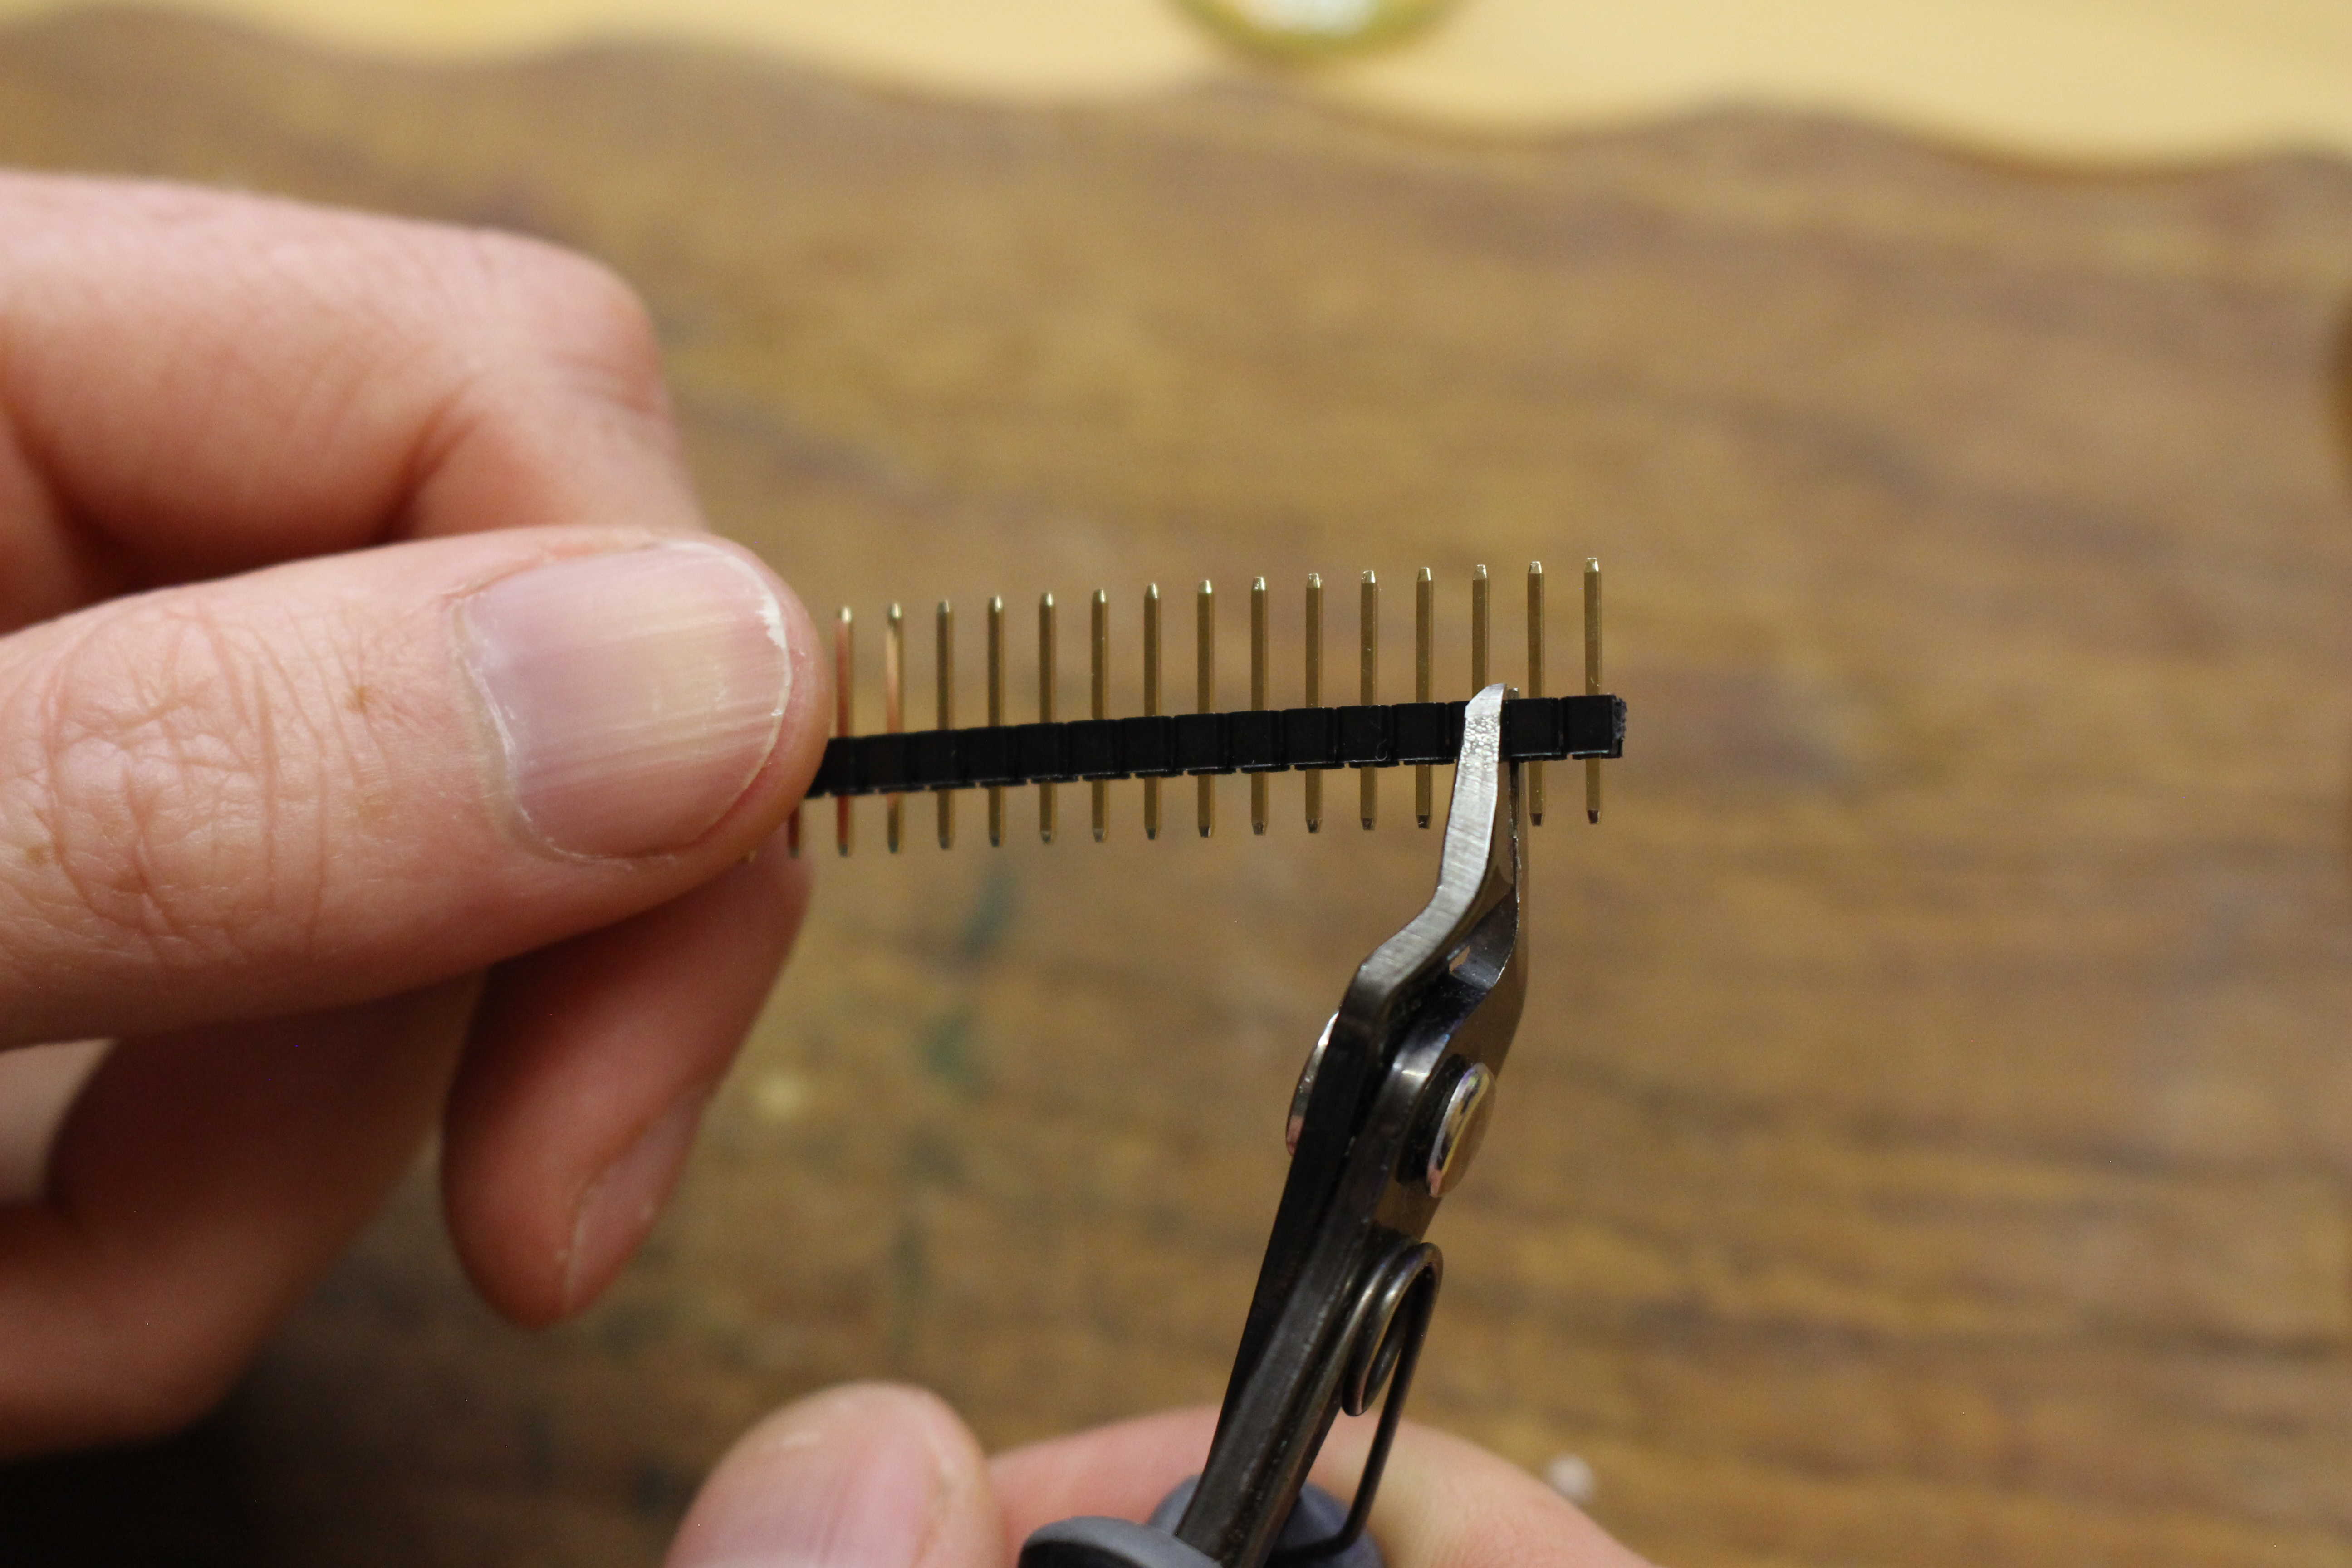
\includegraphics[width=\textwidth]{Bilder/IMG_5603.JPG}
	%\captionof{figure}{}
	%\label{fig:}
\end{minipage}

\vspace{0.5cm}

\begin{minipage}[b]{0.5\textwidth}
	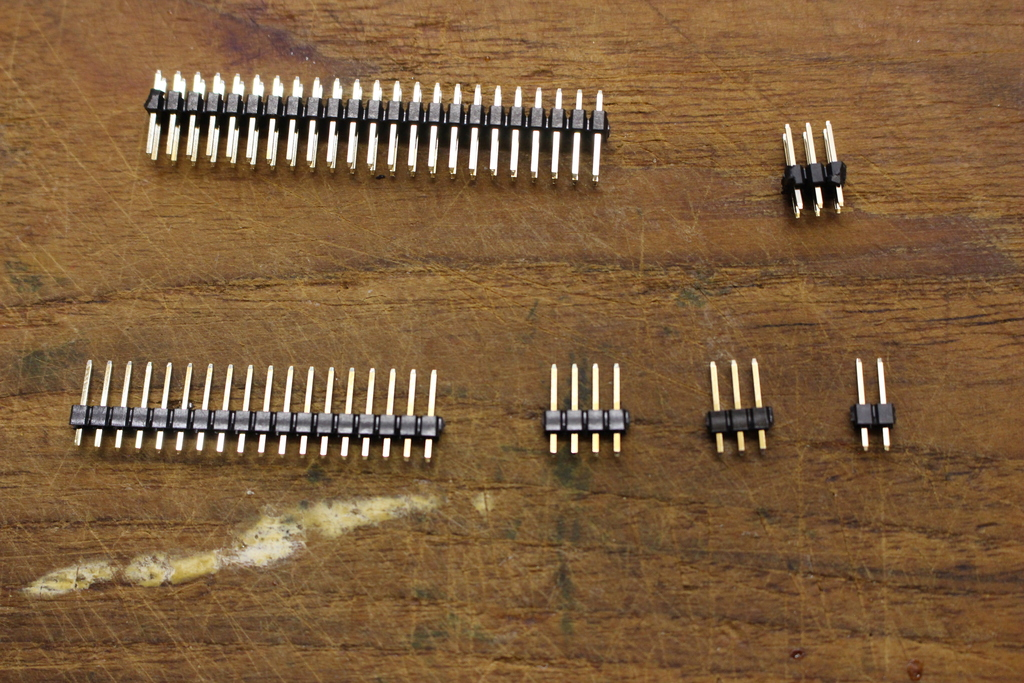
\includegraphics[width=\textwidth]{Bilder/IMG_5604.JPG}
	%\captionof{figure}{}
	%\label{fig:}
\end{minipage}
\begin{minipage}[b]{0.5\textwidth}
	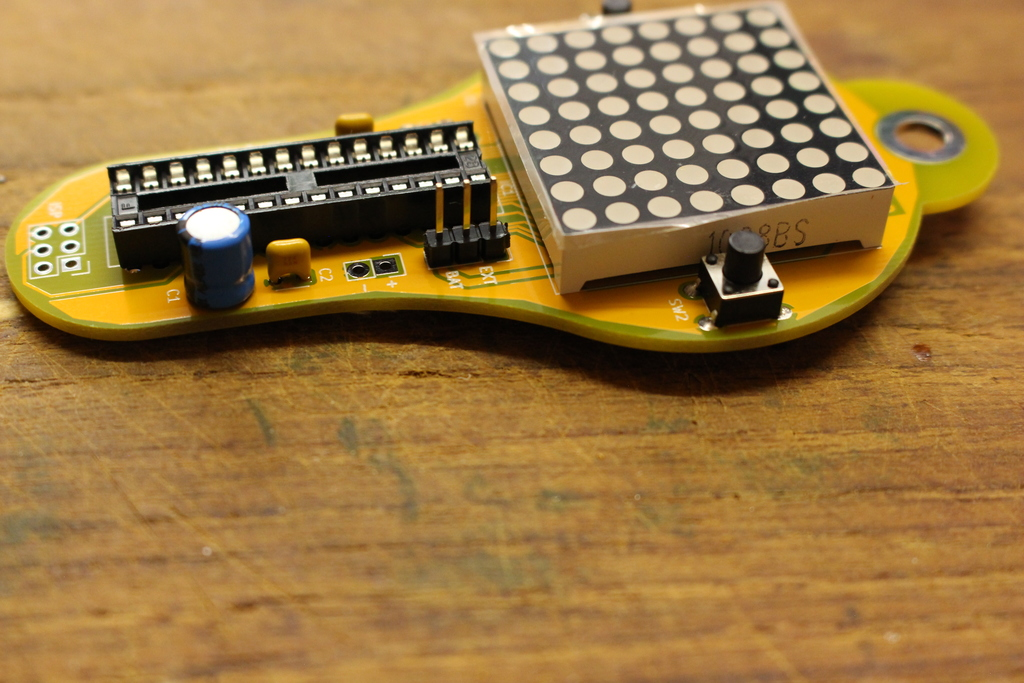
\includegraphics[width=\textwidth]{Bilder/IMG_5605.JPG}
	%\captionof{figure}{}
	%\label{fig:}
\end{minipage}

\vspace{0.5cm}

\begin{minipage}[b]{0.5\textwidth}
	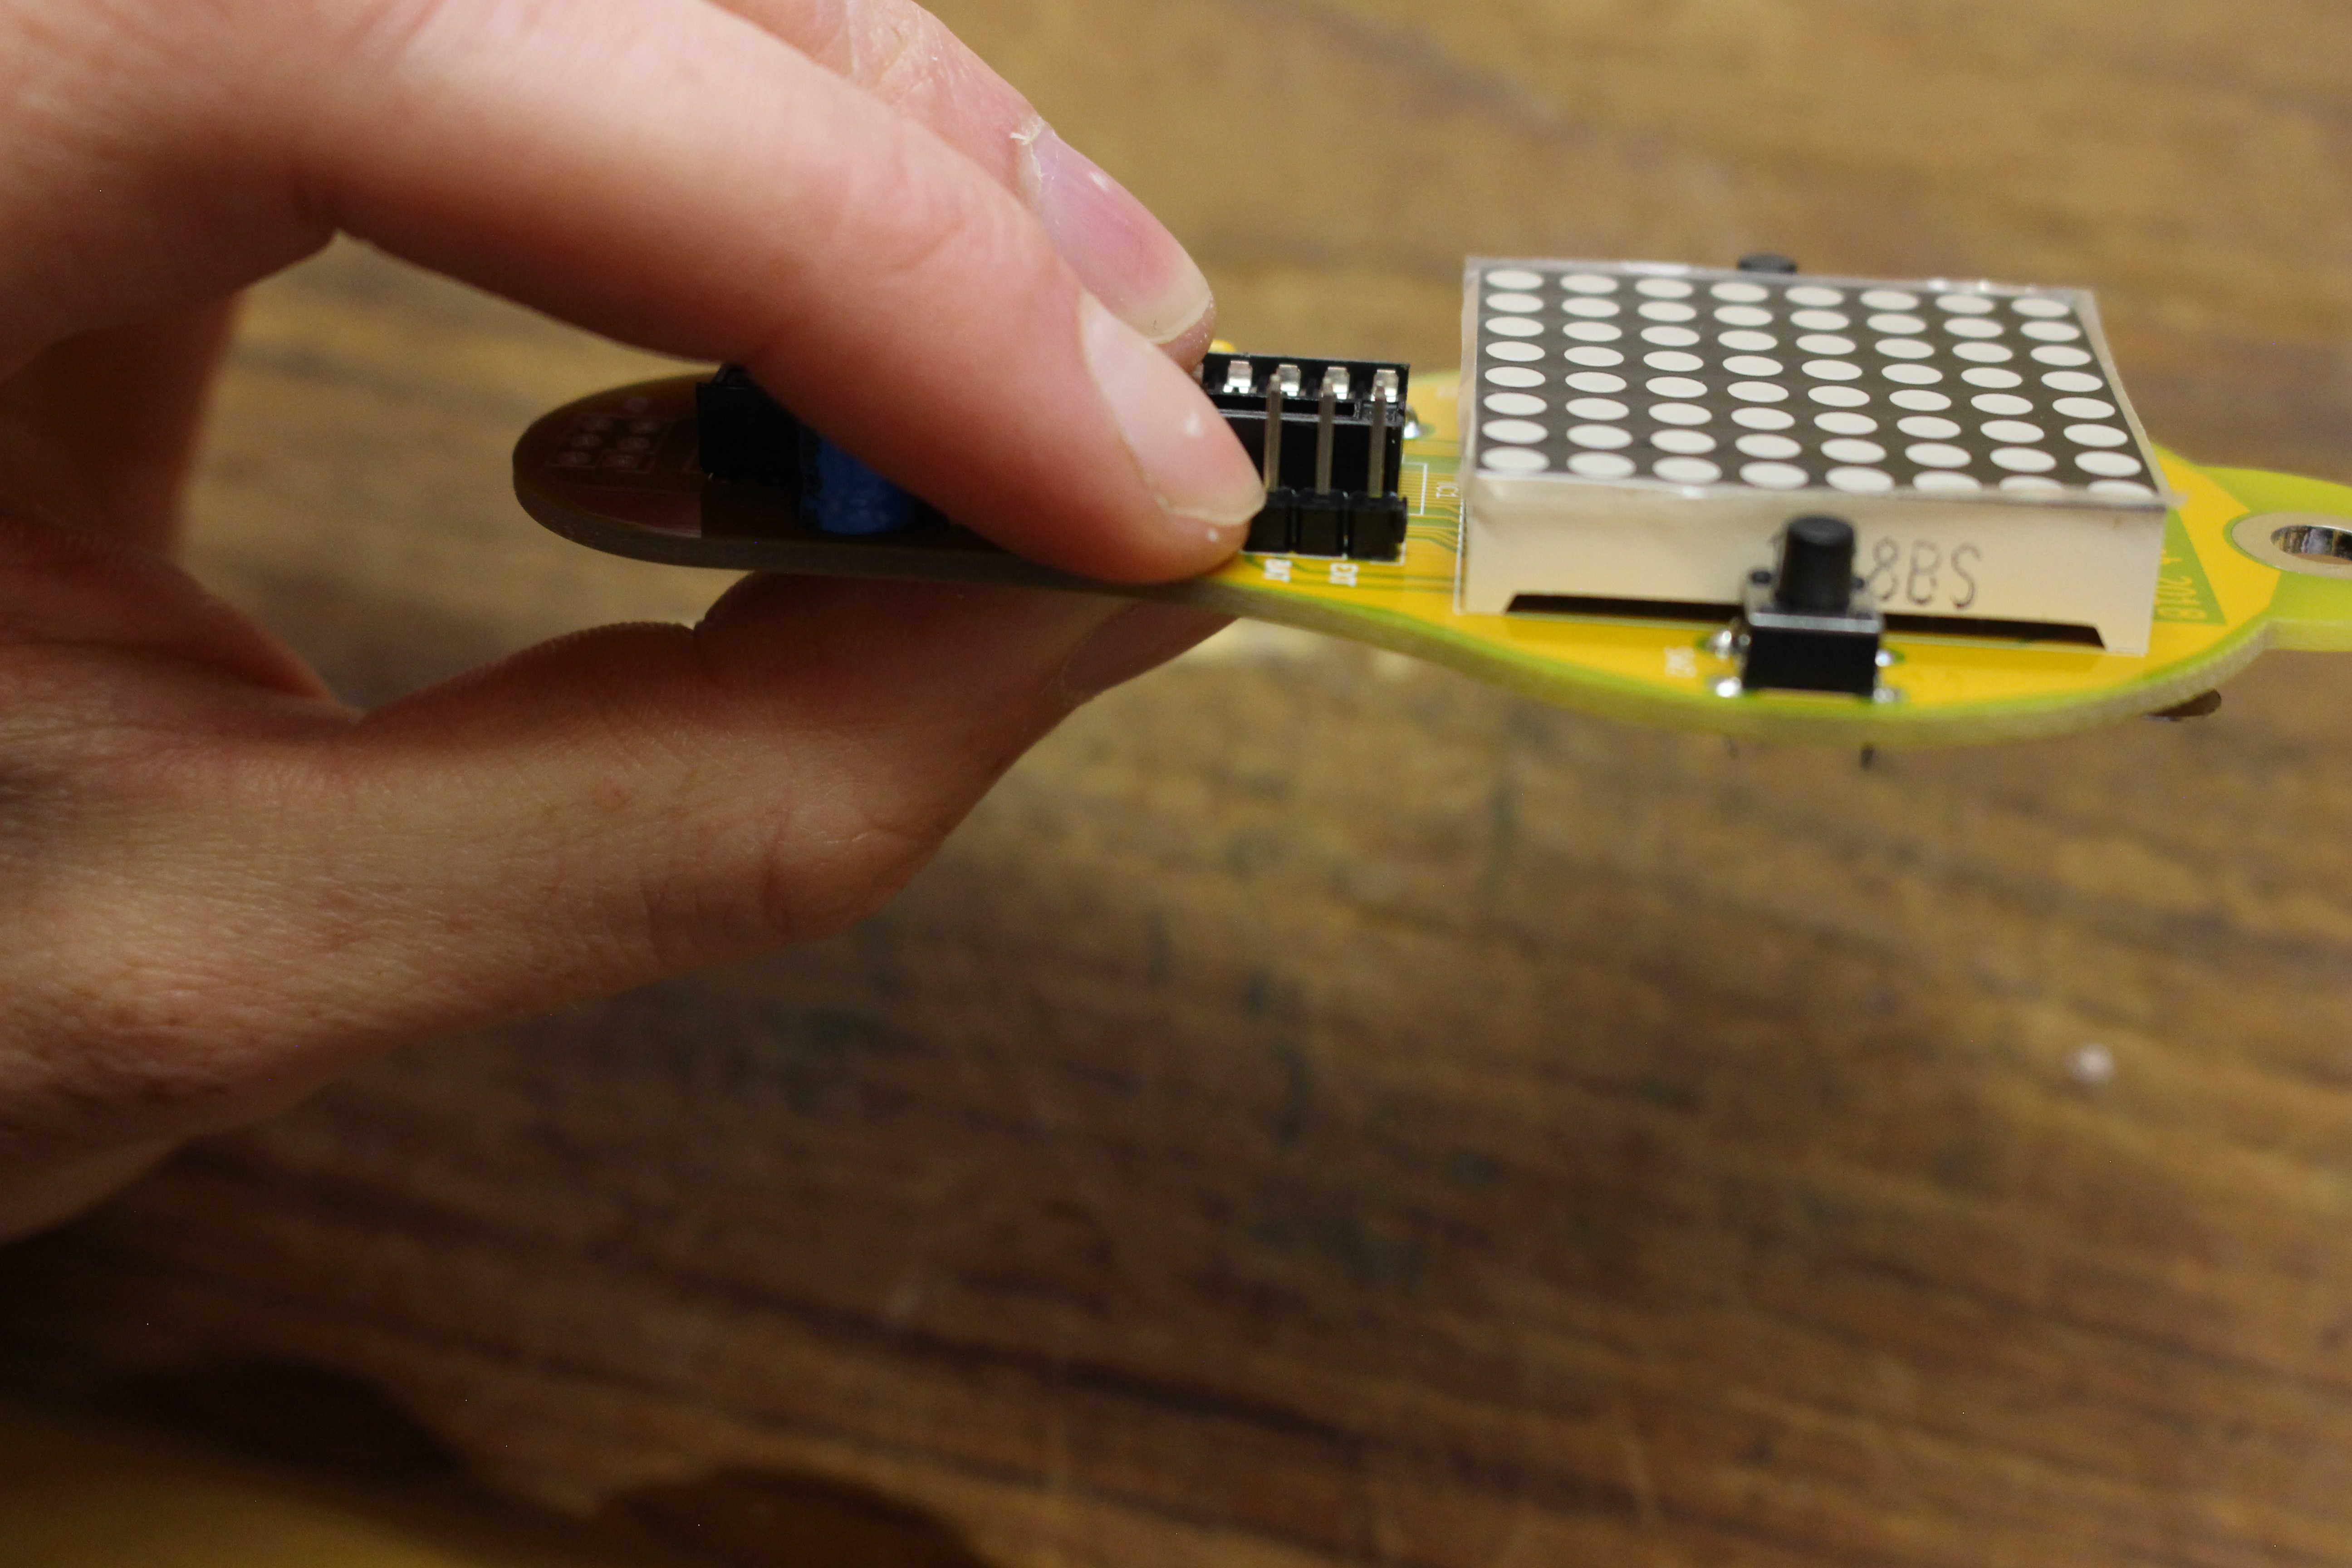
\includegraphics[width=\textwidth]{Bilder/IMG_5606.JPG}
	%\captionof{figure}{}
	%\label{fig:}
\end{minipage}
\begin{minipage}[b]{0.5\textwidth}
	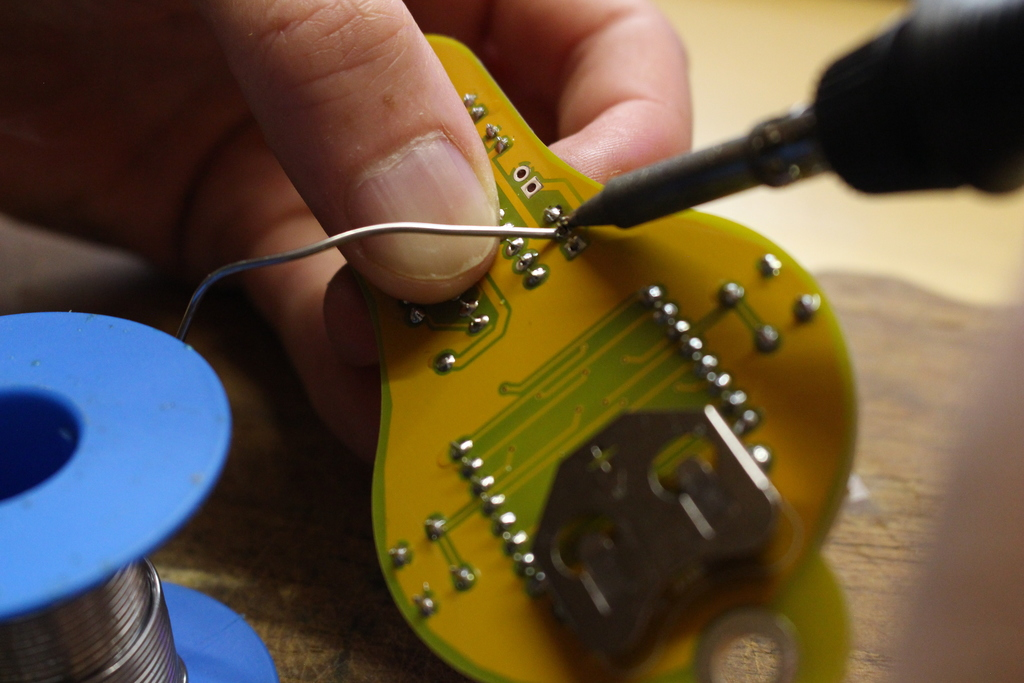
\includegraphics[width=\textwidth]{Bilder/IMG_5608.JPG}
	%\captionof{figure}{}
	%\label{fig:}
\end{minipage}

\vspace{0.5cm}

\begin{minipage}[b]{0.5\textwidth}
	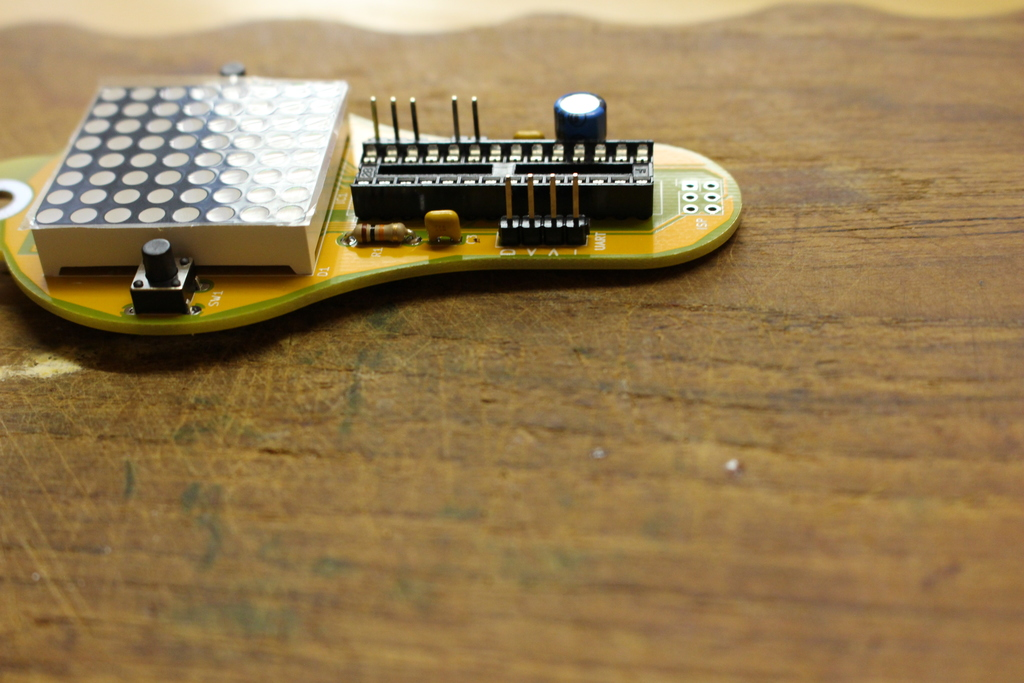
\includegraphics[width=\textwidth]{Bilder/IMG_5612.JPG}
	%\captionof{figure}{}
	%\label{fig:}
\end{minipage}
\begin{minipage}[b]{0.5\textwidth}
	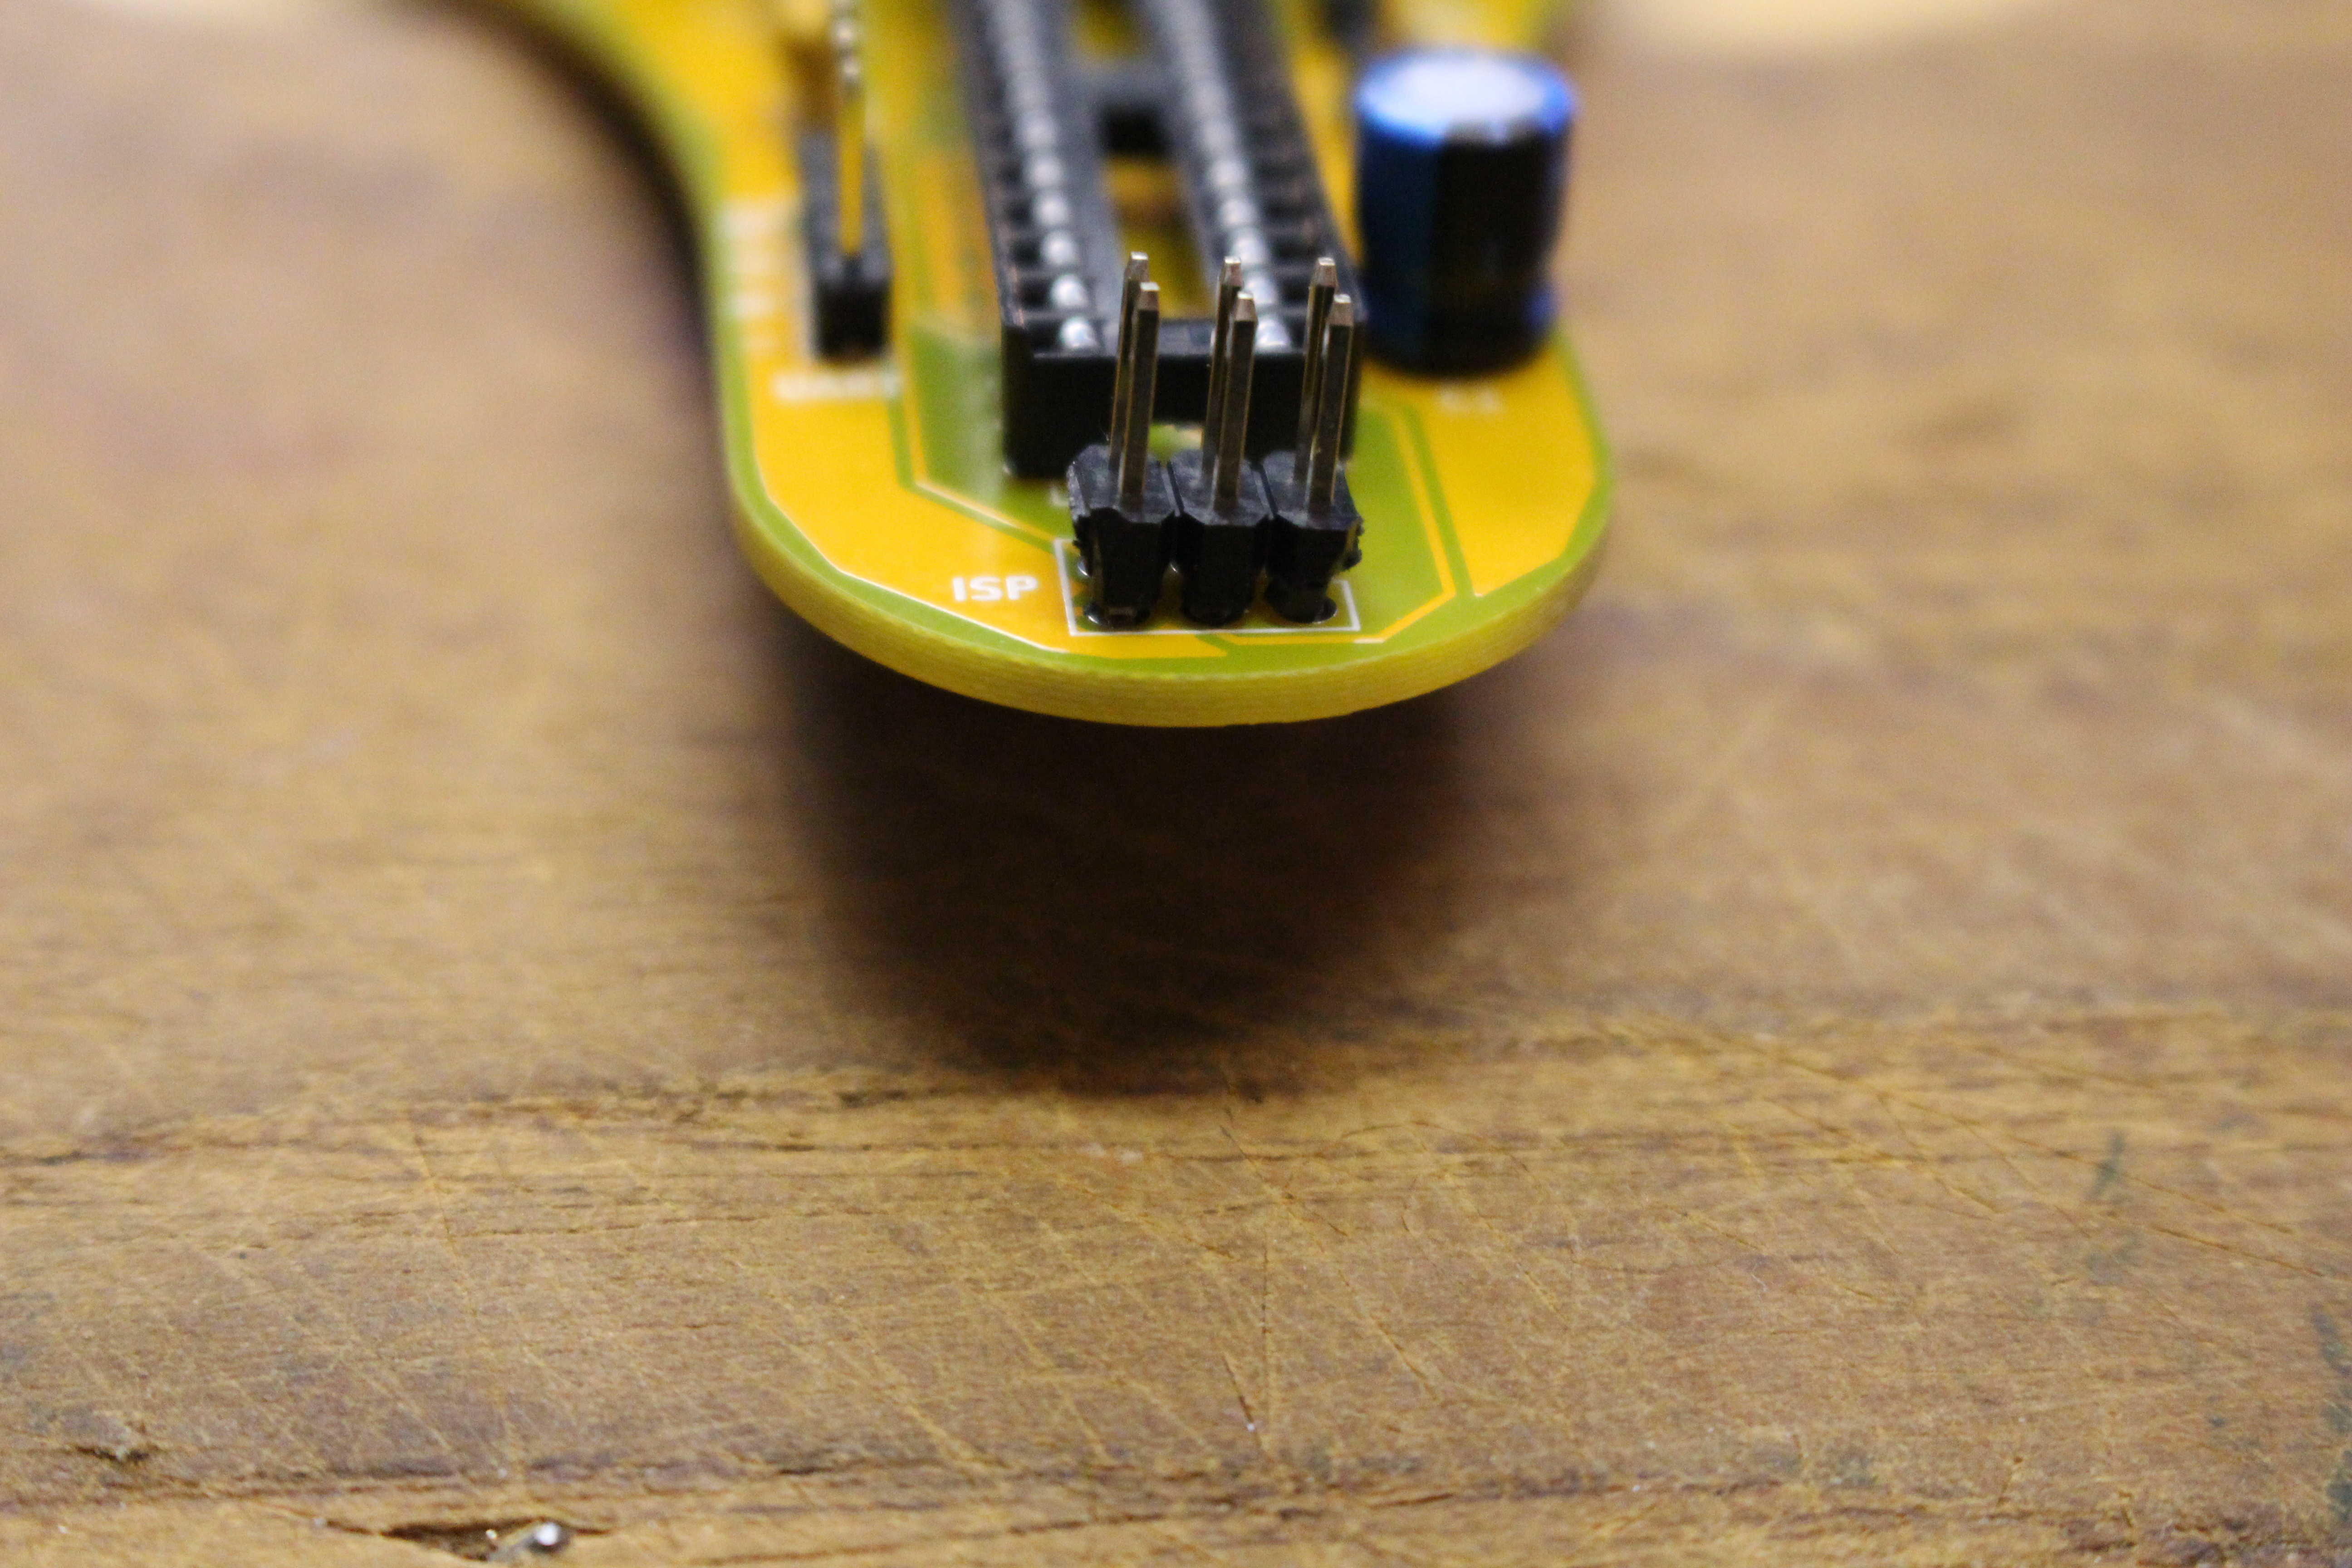
\includegraphics[width=\textwidth]{Bilder/IMG_5616.JPG}
	%\captionof{figure}{}
	%\label{fig:}
\end{minipage}

\section{Den Mikrocontroller programmieren lassen}

Wenn dein Badge fertig gelötet ist, kannst du zur Programmierstation gehen. Dort wird dein Mikrocontroller programmiert und du kannst dir sogar eine individuelle Laufschrift einprogrammieren lassen.

Ist der Controller programmiert, musst du ihn nur noch in den Sockel einsetzen.

Eventuell musst du die Beinchen noch ein wenig zurecht biegen, damit der Controller in den Sockel hineinpasst. 

Dazu legst du den Controller mit einer Pinreihe nach unten auf den Tisch und dem schwarzen Körper zu dir. Dann biegst du den Körper mit beiden Händen von dir weg, so lange bis die Pins nicht mehr schräg nach außen zeigen, sondern nach unten.
Den Vorgang wiederholst du mit der anderen Pinreihe, indem du den Controller einmal umdrehst.

\vspace{1cm}

\begin{minipage}[b]{0.5\textwidth}
	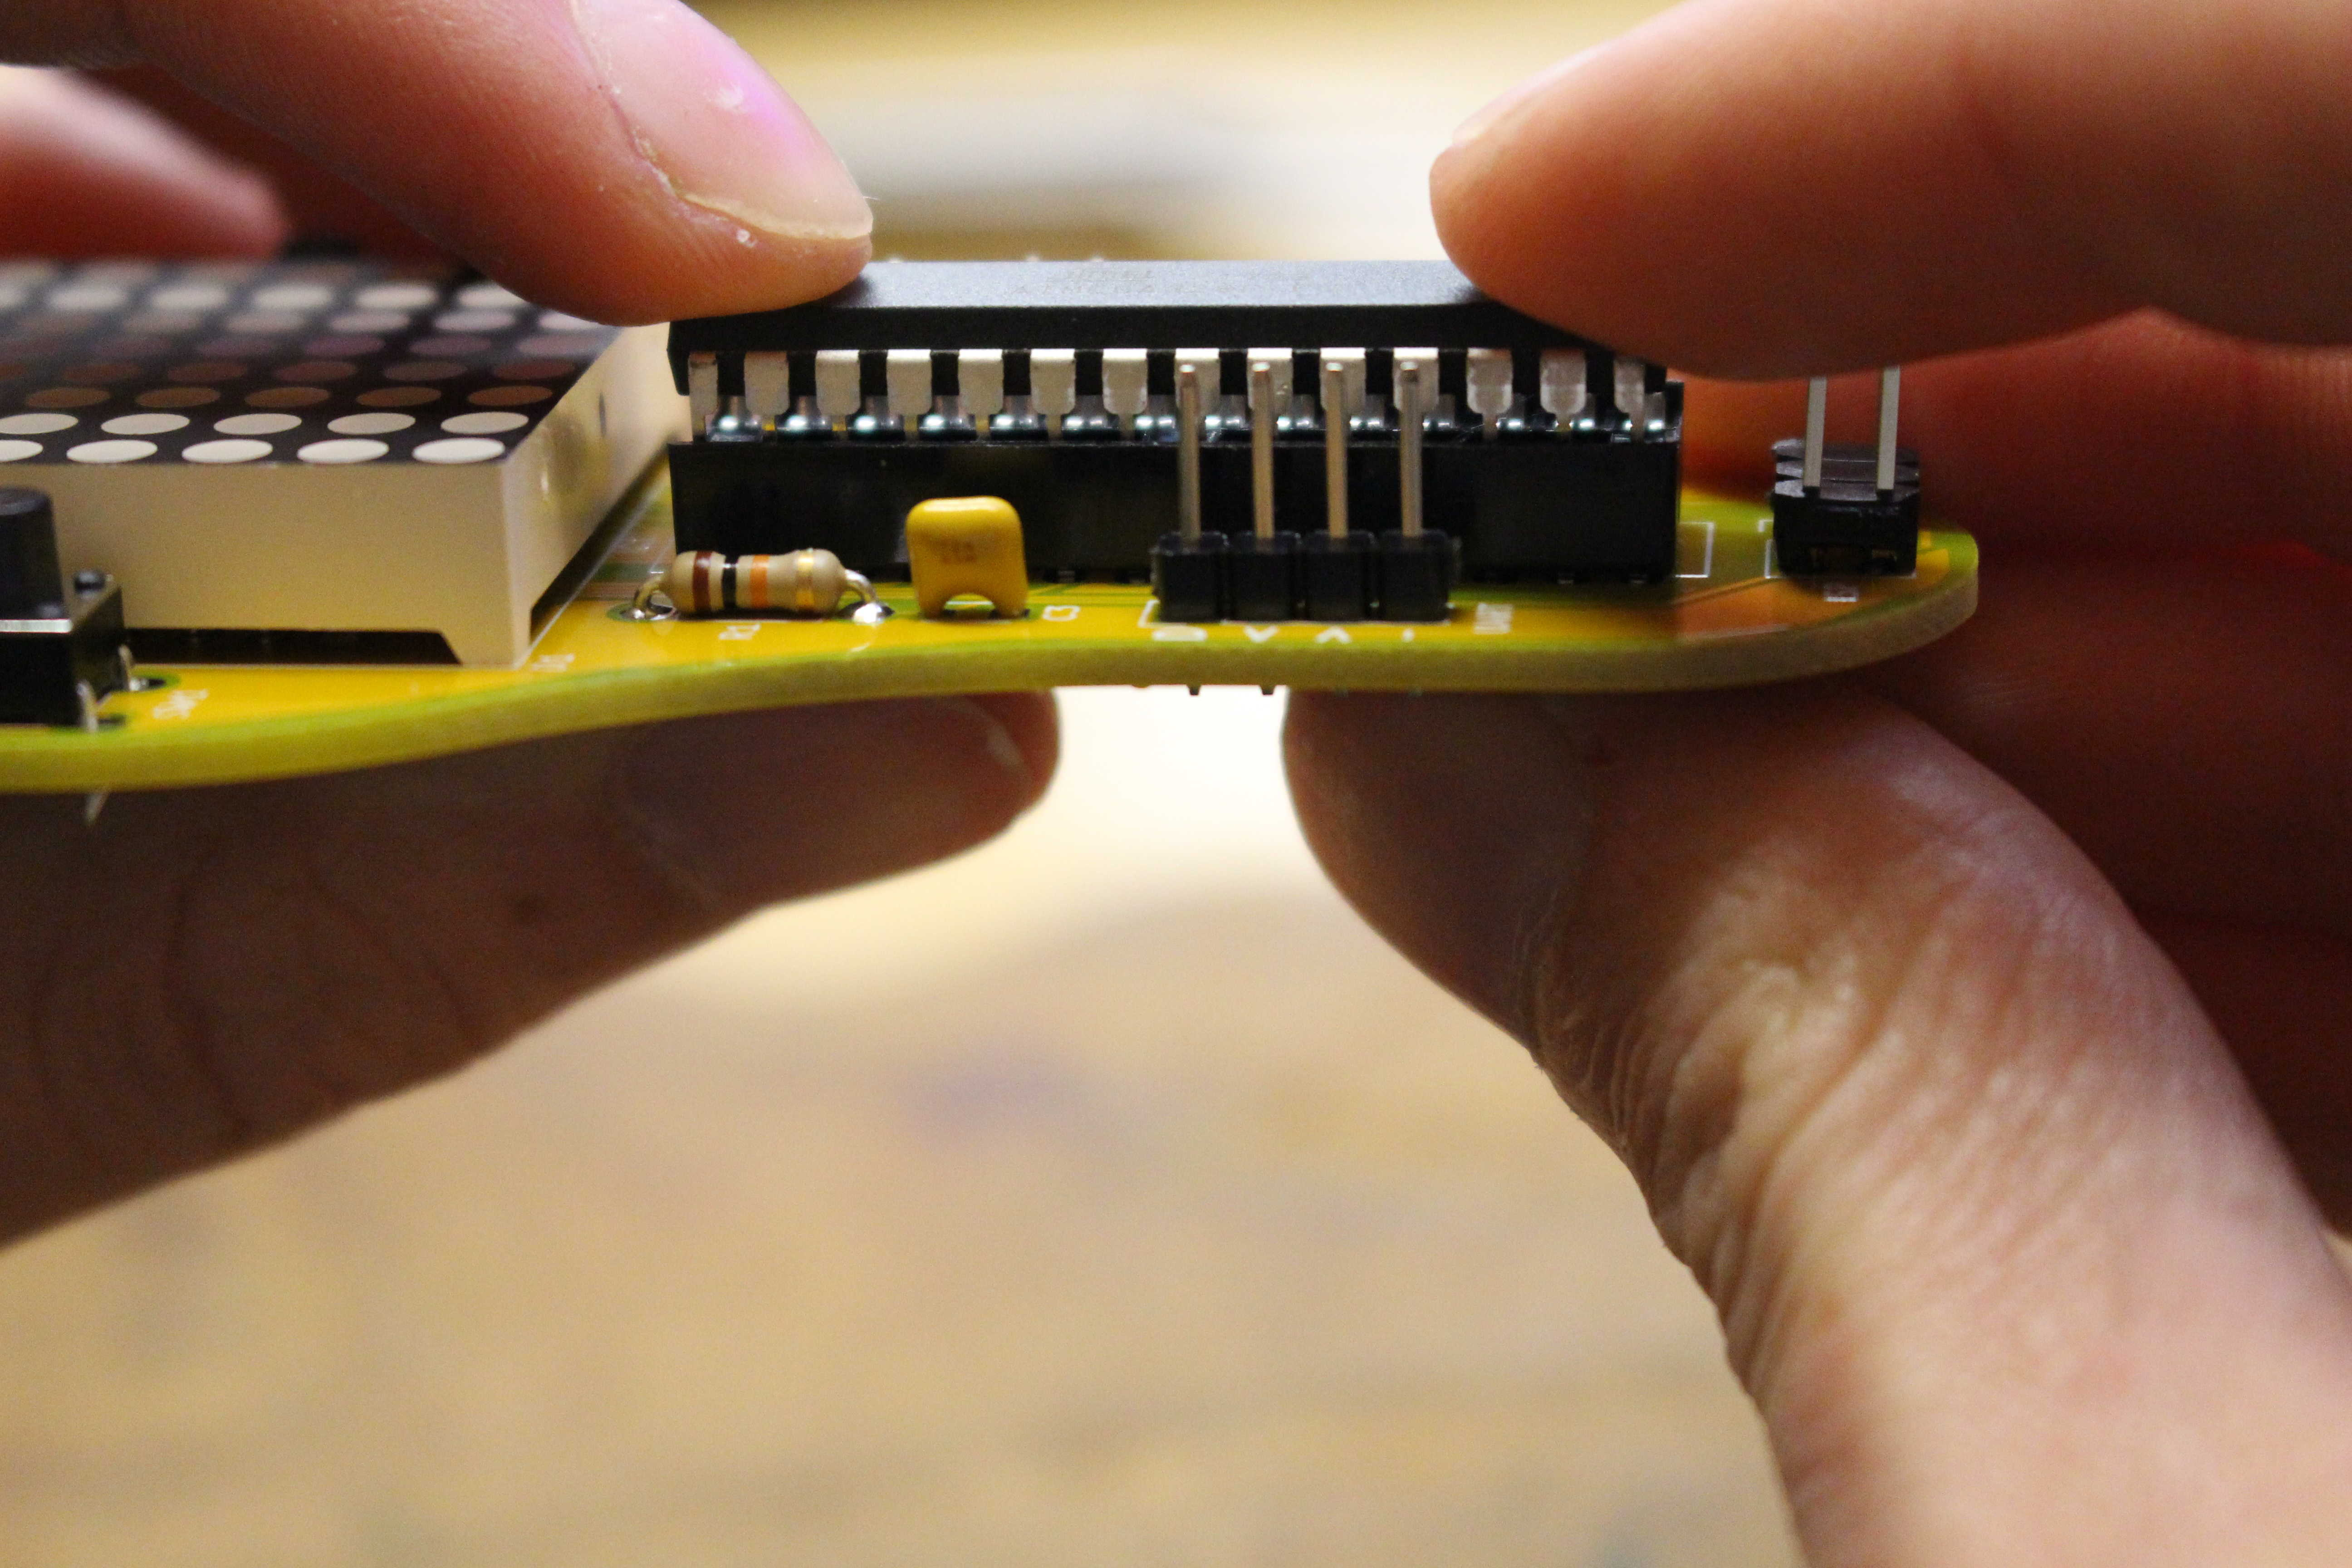
\includegraphics[width=\textwidth]{Bilder/IMG_5620.JPG}
	%\captionof{figure}{}
	%\label{fig:}
\end{minipage}
\begin{minipage}[b]{0.5\textwidth}
	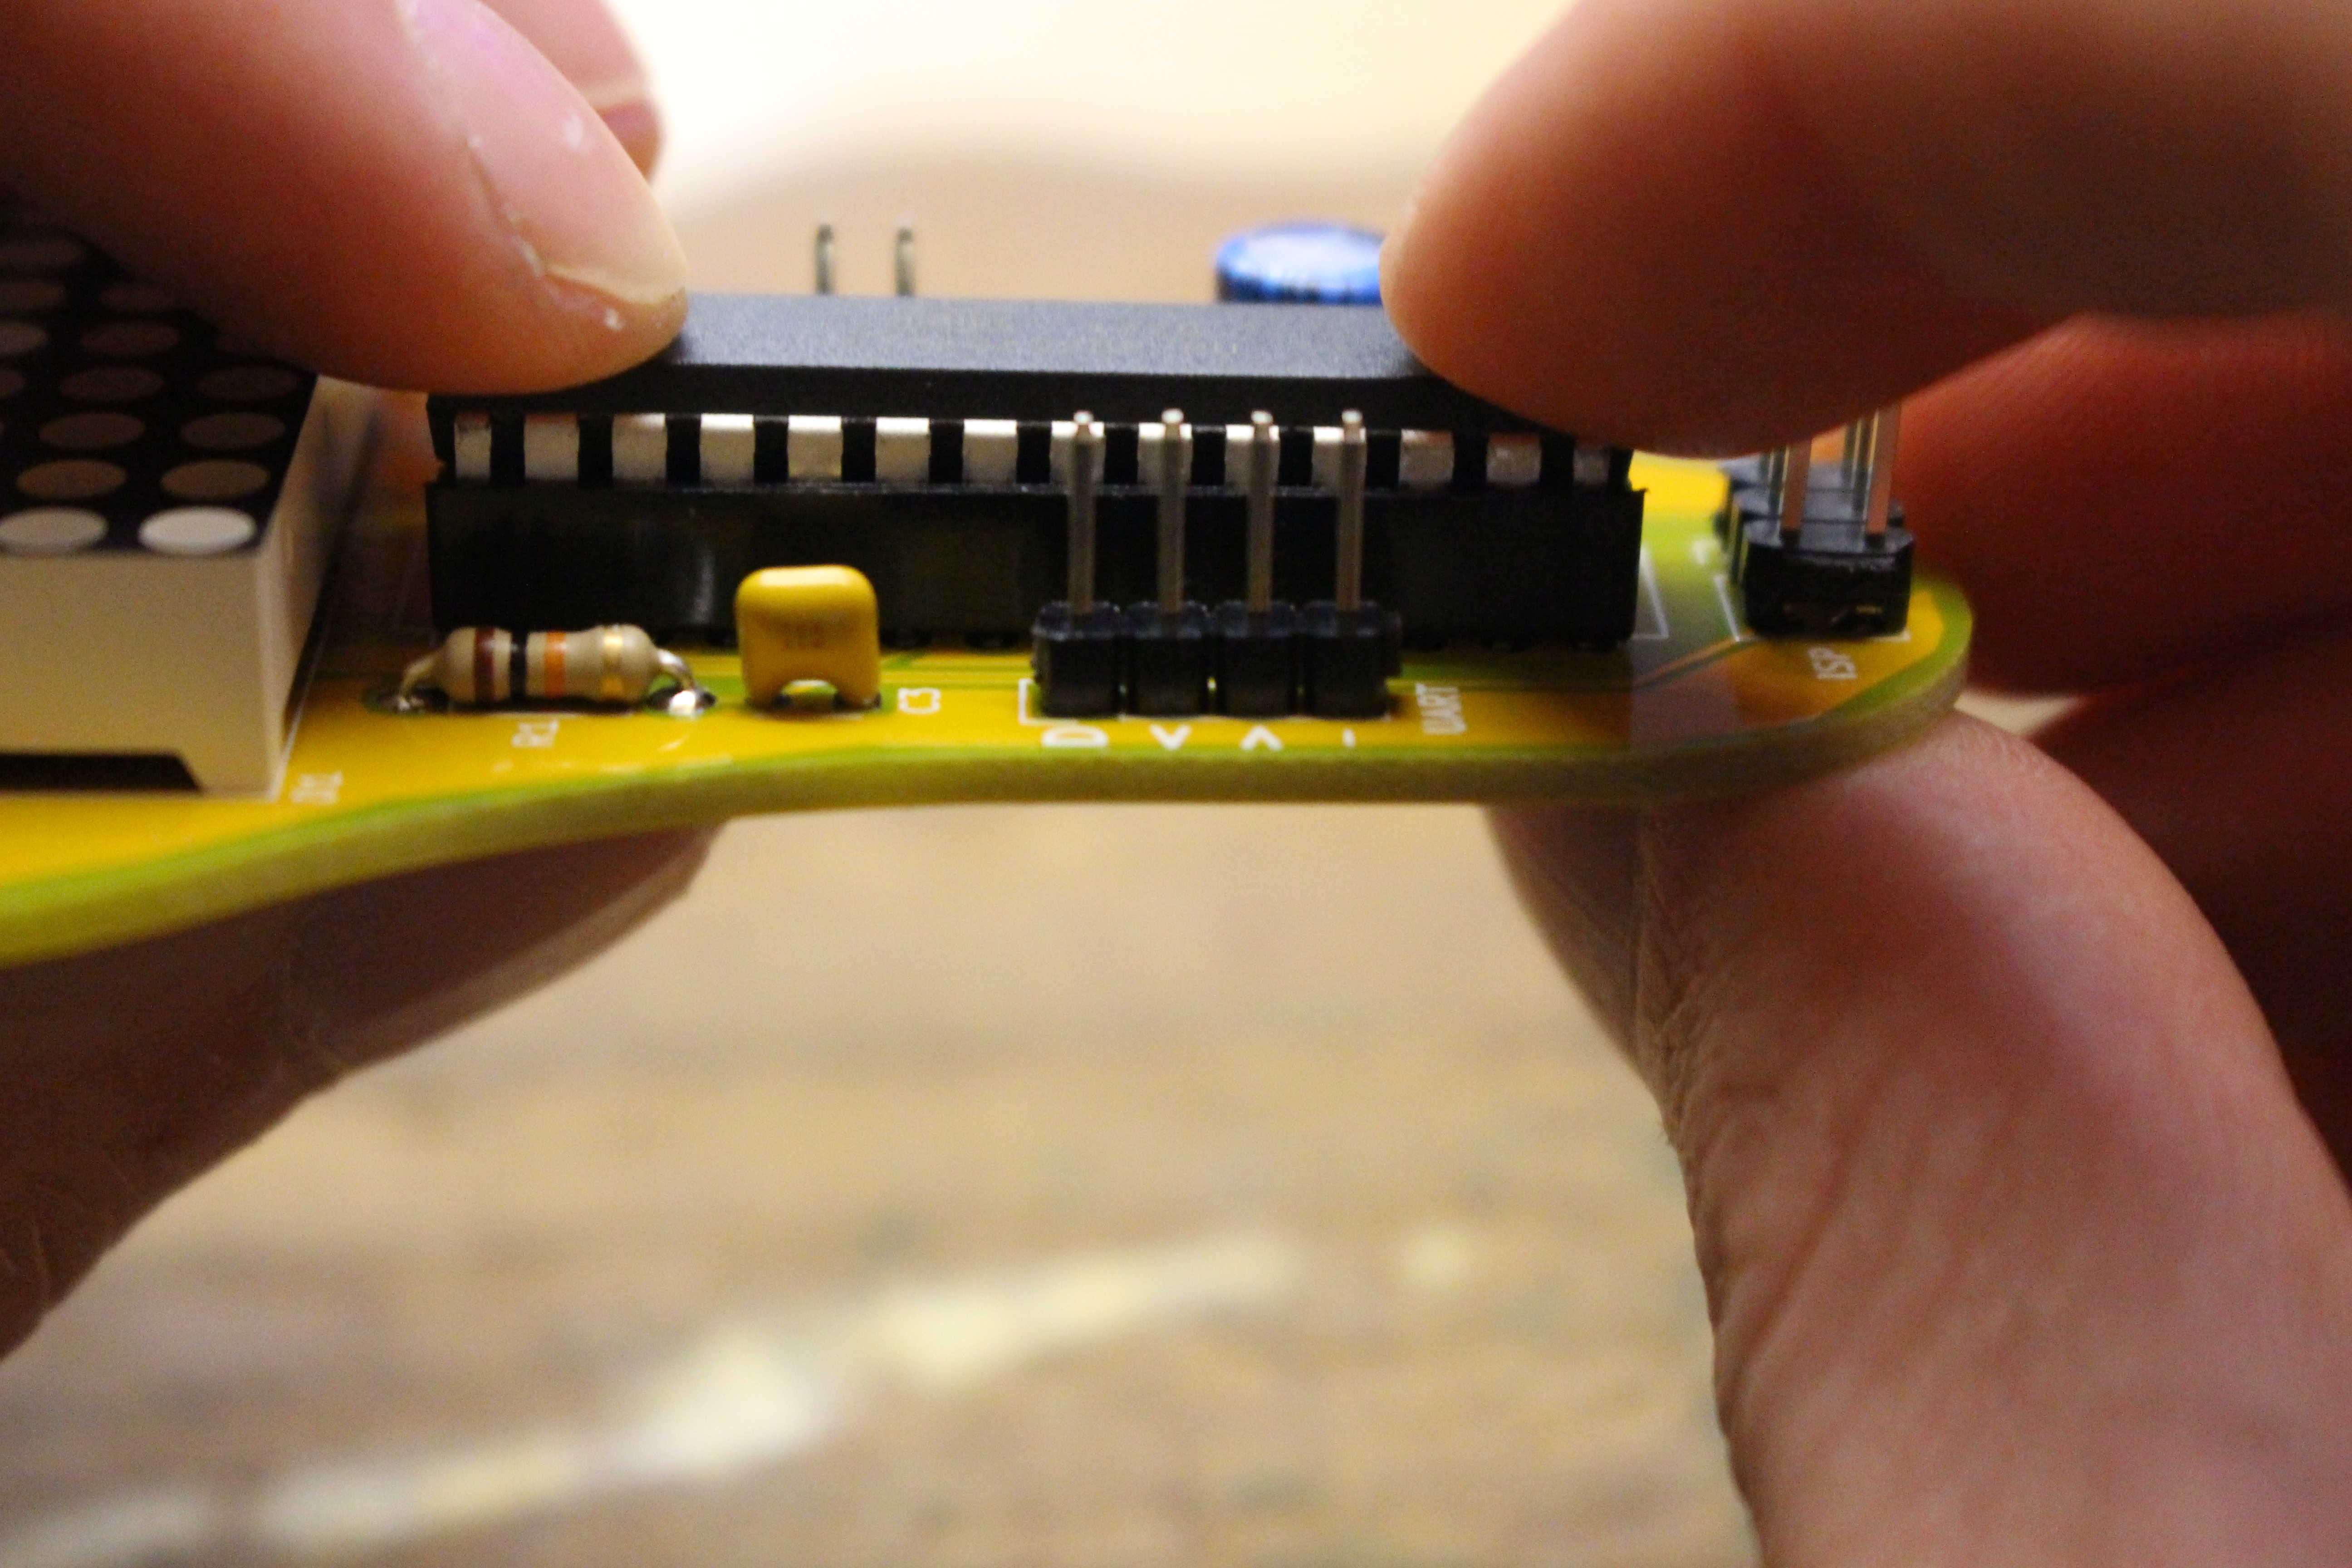
\includegraphics[width=\textwidth]{Bilder/IMG_5622.JPG}
	%\captionof{figure}{}
	%\label{fig:}
\end{minipage}

\section{Der Moment der Wahrheit}

Jetzt musst du nur noch die Knopfzelle in den Knopfzellenhalter schieben.
Achtung! Das Plus-Zeichen muss nach oben schauen.

Zum Schluss den Jumper auf die 3-Polige Stiftleiste setzen, wo die Markierung BAT zu sehen ist.

Jetzt sollte dein Badge anfangen wie wild zu blinken.

\vspace{1cm}

\begin{minipage}[b]{0.5\textwidth}
	\includegraphics[width=\textwidth]{Bilder/IMG_5625.JPG}
	%\captionof{figure}{}
	%\label{fig:}
\end{minipage}
\begin{minipage}[b]{0.5\textwidth}
	\includegraphics[width=\textwidth]{Bilder/IMG_5626.JPG}
	%\captionof{figure}{}
	%\label{fig:}
\end{minipage}

\vspace{0.5cm}

\begin{minipage}[b]{0.5\textwidth}
	\includegraphics[width=\textwidth]{Bilder/IMG_5627.JPG}
	%\captionof{figure}{}
	%\label{fig:}
\end{minipage}
\begin{minipage}[b]{0.5\textwidth}
	\includegraphics[width=\textwidth]{Bilder/IMG_5628.JPG}
	%\captionof{figure}{}
	%\label{fig:}
\end{minipage}

\vspace{0.5cm}

\begin{minipage}[b]{0.5\textwidth}
	\includegraphics[width=\textwidth]{Bilder/IMG_5629.JPG}
	%\captionof{figure}{}
	%\label{fig:}
\end{minipage}
\begin{minipage}[b]{0.5\textwidth}
	\includegraphics[width=\textwidth]{Bilder/IMG_5634.JPG}
	%\captionof{figure}{}
	%\label{fig:}
\end{minipage}

\section{Was tut es?}

Auf dem Badge sind mehrere kleine Programme installiert. Um sie umzuschalten, musst du beide Taster gleichzeitig für 3 Sekunden gedrückt halten.\\

\textbf{Laufschrift:}\\
Zeigt den Text an, den du in das Badge hast programmieren lassen.\\

\textbf{Psychedelische Spirale:}\\
Nicht zu lange drauf schauen!!!\\

\textbf{Random:}\\
Alles reiner Zufall.\\

\textbf{Pong:}\\
TO BE DONE\\

\textbf{Crazy Snake:}\\
Die Schlange macht lustige Runden über das Display, am einen Rand raus, am anderen wieder rein. Sie stößt mit sich selbst nicht zusammen und ist darum unsterblich. Je länger sie wird, um so schneller flitzt sie rum und wenn sie alt wird verzehrt sie sich langsam wieder selbst. Endloser Spaß für die ganze Familie!\\

Mit den beiden Tastern kann man die Schlange nach links und rechts abbigen lassen und so versuchen die Mäuse zu fangen.\\

\bibliographystyle{plain}
\bibliography{references}
\end{document}